%%**************************************************************************************************
%%
%% File Name : Math_Top.tex
%% 説明      : 数学ノートの構成を明記するファイル
%%
%%**************************************************************************************************
%===================================================================================================
%  Part : 数学の勉強ノート
%  説明 : 物理学で使われる数学について記述する.
%===================================================================================================
    \part{数学の勉強ノート}
%   %-----------------------------------------------------------------------------------------------
%   %  Input
%   %    File Name : PhysNote_Math.tex
%   %    説明      : 数学のトップファイル.
%   %                予め知っておくべき,数学について記述する.
%   %-----------------------------------------------------------------------------------------------
        %%**************************************************************************************************
%%
%% File Name : PhysNote_Math.tex
%% 説明      : 予め知っておくべき,数学的知識を確認する
%%
%%**************************************************************************************************

%===================================================================================================
%  Chapter : はじめに
%  説明    : 数学の学習マップを記述する.動機付けも含めて.
%===================================================================================================
\chapter{はじめに}
%   %-----------------------------------------------------------------------------------------------
%   %  Input
%   %    File Name : PhysNote_Math_MsgFirst.tex
%   %    説明      : 数学の学習マップを記述する.動機付けも含めて.
%   %-----------------------------------------------------------------------------------------------
        %===================================================================================================
%  Chapter : はじめに
%  説明    : 数学の学習マップを記述する.動機付けも含めて.
%===================================================================================================

%   %==========================================================================
%   %  Section
%   %==========================================================================
        \section{物理学と数学}
            物理学の勉強を始めようとしているのに,なぜその前に数学を勉強しなければ
            ならないのか.
            あるいは,なぜ,物理学の学習と,数学の学習を同時に進めないといけないのか.
            それは,物理学では数学を道具として扱うからである.その道具の使い方を
            知らずして,物理学は学習できないのである.

            もちろん,近代物理学の創始者ニュートン
                \footnote{
                    Sir Isaac Newton(1643--1727, イギリス):古典力学の創始者.
                    微分法という就学的手法を発明し,物体の運動を記述することがで
                    きるようになった.彼の名をとって,「ニュートン力学」とよばれ
                    ることも多い.また後で,ニュートン力学の部分において,紹介す
                    ることになろう.
                }
            の時代には,物理学のための数学なんてものはなく,物理学の研究に伴って,
            その数学的手法である微分積分学を作る必要があった.数学的手法の発明時
            には記号の統一ができていなかったり,不明確な問題も多いものである.そ
            してこれらの問題は,後の時代の多くの数学者によって解決され,その表現
            方法もよりわかりやすい形に書き改められ,きれいな体系に整えられていく.
            そのため,ニュートンの理論の数学的表現は現在とは全く異なる.現在の物
            理学で用いられる数学は,代数学や微分積分学がある
                \footnote{
                    特に,微分積分学はニュートンが物理学を構築するために発明され
                    た数学的手法である.(ライプニッツも同時期に微分積分学を発明
                    している.)微分積分学の発明当時には,極限の定義が曖昧であっ
                    たり,使用される記号も分かりにくいものであった.
                }.
            現在の物理学は,これらが当たり前のように使われる.いわば,物理学を記
            述するために欠くことのできない言語なのである
                \footnote{
                    物理学は数学の助けを借りて成立している.
                }.
            だから,物理学を学習する前に,まずは最低限の数学を学習する必要がある.

            物理学を学んでいく途中で,必要になったらその数学を学ぶという方法もあ
            るが,ある程度の数学的知識を予め身に着けておいた方が,学習するのに効
            率的である.「ある程度」を見極めるのは難しいが,ここではさしあたり,
            高校レベルの数学がわかるくらいを目標に,数学を学ぶ.


%   %==========================================================================
%   %  Section
%   %==========================================================================
        \section{「数学的準備」の学習マップ}
            このPertで学習する数学について,簡単に触れておこう.まず,内容を列挙
            してみよう.
                \begin{enumerate}
                    \item 関数
                    \item 微分積分学
                    \item 微分方程式
                    \item ベクトル
                    \item ベクトル解析(ベクトルの微分積分)
                    \item 行列
                \end{enumerate}

            まず,「関数」を学習する.中学校では,1次関数や2次関数に触れたこと
            と思う.ここでは,これらをもう少し一般的に考える.物理学ではこの関数
            がメインとなる.関数により,自然法則を記述するからである.

            次に,「微分積分学」を学習する.ただし,深入りはしない.図形的直感を
            第一に考える.物理学は物体の運動や挙動を数式で表現することがその目的
            のひとつである.つまり,物体の位置の時間的な変化を記述できなければい
            けない.この時間変化を表現する最善の手段として,ニュートンは微分積分
            法という新しい数学分野を開拓した.

            その次に,「微分方程式」について学習する.微分方程式とは,微分積分法で
            定義される微分を含む数式のことである.通常の方程式では,未知変数 $x$ や $y$ が
            方程式を満たす値を求める.これに対して,微分方程式で,未知変数に対応する
            のが,未知関数である.微分方程式を解くということは,その微分方程式を
            満たす関数の具体的な形を求めることにほかならない.

            その次に,「ベクトル」について学習する.ベクトル
            は,物体の位置を数学的に表現するものである.これも図形的イメージ習得
            を第一にする.

            その次に,「ベクトル解析」を学習する.ベクトル解析は,ベクトルに微分積
            分学を組み合わせたものであるとも言えよう.ベクトルは物体の位置を表現
            するものであり,微分積分学は時間的変化を記述するものである.つまり,
            ベクトルに対して,微分積分を適用すると,物体の位置の時間変化を数学的
            に扱うことができるようになるのだ.

            その次に,「行列」を学習する.行列とは,何個かの数を縦横に並べてひとつの
            組として扱われるものである.行列の概念は,言葉で説明するよりも,具体例を
            示したほうが分かりやすいだろう.以下は,行列の具体的な例である.
            \begin{equation*}
                \begin{bmatrix}
                    a_{00} & a_{01} \\
                    a_{10} & a_{11}
                \end{bmatrix}
                \;\;\;,\,\;
                \begin{bmatrix}
                    a_{00} & a_{01} & a_{02} \\
                    a_{10} & a_{11} & a_{12}
                \end{bmatrix}
                \;\;\;,\,\;
                \begin{bmatrix}
                    a_{00} & a_{01} & a_{02} \\
                    a_{10} & a_{11} & a_{12} \\
                    a_{20} & a_{21} & a_{22}
                \end{bmatrix}
            \end{equation*}
            これらについての,具体的な性質について考えることは,行列という数学分野である.
            しかしここでは,行列というものの具体的な形を紹介しただけにとどめておこう.
            具体的な定義や性質は,後で考えることにする.


%===================================================================================================
%  Chapter : 関数
%  説明    : 関数の考え方を確認する.
%===================================================================================================
\chapter{関数}
%   %-----------------------------------------------------------------------------------------------
%   %  Input
%   %    File Name : PhysNote_Math_Function.tex
%   %    説明      : 「関数」について.考え方と使い方.
%   %-----------------------------------------------------------------------------------------------
        %===================================================================================================
%  Chapter : 関数
%  説明    : 関数の考え方を確認する.
%===================================================================================================

%   %==========================================================================
%   %  Section : 集合
%   %==========================================================================
        \section{集合}
%       %----------------------------------------------------------------------
%       %  Input
%       %    File Name : PhysNote_Math_Function_Set.tex
%       %    説明      : 素朴な集合論を考える(公理的には扱わない)
%       %----------------------------------------------------------------------
        %   %==========================================================================
%   %  Section : 集合
%   %==========================================================================
        %==================================================================
        %  SubSection
        %==================================================================
            \subsection{集合を定義するとは}
                数学において,\textbf{集合} とは,その最も基礎にあたる概念である.
                数学の要である自然数も,集合という概念を使って定義されるものである.
                自然数の定義は,\textbf{ペアノ
                    \footnote{
                        Giuseppe Peano(1858--1932, イタリア):数学者.自然数を作り出
                        す仕組みである「ペアノの公理系」を提案する.
                    }
                の公理系}として知られている
                    \footnote{
                        ここでは,集合の重要性を示すことが目的なので,
                        ペアノの公理は解説しない.
                        ペアノの公理系を解説するWebサイトは非常に多いし,
                        整数論などの数学の教科書には必ず記述されているので,
                        それらを参照してもらいたい.
                    }.

                集合が数学の最も基礎的な概念であるだけに,それを定義することは
                非常に難しい.中学校や高校で集合について学習するとき,次のように
                集合という概念が説明される.
                    \begin{description}
                        \item[中学・高校での集合の定義] 「集合とは,モノの集まりである.
                        ただし,ここで言うモノとは,集合に属するか否かを明確に判断できる
                        ものに限る.」
                    \end{description}

                この集合の定義は,直観的で非常に分かりやすい.しかし,この“ただ
                し”以下の部分に問題がある.“モノが集合に属すか否かを明確に判断
                できる”とは,どういうことか.「自然数」や「有理数」などは,明確な
                判断が下せるので,モノである.しかし,「美人」とか「厳密」だとか
                というのは,万人に対して明確な判断基準を与えることができず,モノ
                ではありえない.となると,どういった場合に,モノになりうるのかと
                いう疑問が自然と脳裏にうかんでくる.しかし,実際問題として,モノ
                になりうるかどうかの判断基準を明示することは不可能なのである.
                つまり,「モノの集まりを集合という」といった集合の定義は,深く考
                えると曖昧な部分が浮き彫りにされてくるのである
                    \footnote{
                        \textbf{集合論が含む矛盾}\;\;\;たしかに,集合論(特に無限集合論)
                        の開拓者であるカントール
                        (※1)が与えた集合の定義は「モノの集まりを集合という」であった.
                        しかし,この定義を用いると,矛盾したことが起こってしまうことをラッセル(※2)が
                        発見した.この矛盾したこととは,次のような命題(定義A)を考える
                        ことで説明される.
                        \begin{itemize}
                            \item
                                \textbf{定義A}:「自分自身を含まない全ての集合を $\omega$ とする」
                        \end{itemize}

                        さて,どこが矛盾なのかを説明しよう.次の問題を考えてみる.
                        \begin{itemize}
                            \item
                                \textbf{問題X}:「$\omega$ は,$\omega$ 自身に含まれるか,否か」
                        \end{itemize}

                        考えらる答えは2つしかない.1.)含まれるか,2.)含まれないか,のどちらか
                        である.さて,1.)の状況,つまり,$\omega$ は $\omega$ 自身に含まれる
                        と仮定しよう.この場合,定義Aにより自分自身を含まない.しかし,いま,
                        $\omega$ 自身に含まれているという仮定に反する.つまり,「1.)含まれる」
                        は間違いである.では,2.)の状況,つまり,$\omega$ は $\omega$ 自身に含
                        まれないが答えなのだろうか.しかし,この場合,定義Aに反していることは明
                        白であり,「2.)含まれない」も間違いである.考えられるすべての答えで前提
                        とする条件と矛盾する結果がでてしまう.これを \textbf{ラッセルのパラド
                        クス} という.どう考えても,定義Aによって作られる集合 $\omega$ は問題Xを
                        突きつけられると,その答えは矛盾を生じるという結果に終わる.

                        これは致命的な問題である.集合はすべての数学の分野の基礎にあたる概念で
                        あり,この部分に欠陥があるということは,すべての数学分野の存立が危うく
                        なる.

                        ここで示した矛盾以外以外にも,カントール自身が発見した \textbf{カントー
                        ルのパラドクス} がある.任意の集合 $A$ に対し,それよりも大きい集合を
                        作成できることが証明されている(「集合の集合」を考えることができてしまうので).
                        にもかかわらず,最大の大きさを持つ集合
                        があることも証明されてしまった.つまり,いくらでも大きい集合を考えること
                        ができると保証されているのに,その大きさには上限があるという.明らかに,
                        矛盾している.(自然数を例として言えば,「自然数はいくらでも大きい数を創
                        りだすことができるのに,それには最大値がある」と言っているのと同じである)

                            (※1)カントール:Georg Ferdinand Ludwig Philipp Cantor(1845--1918, ロシア)

                            (※2)ラッセル:Bertrand Arthur William Russell(1872--1970, イギリス)
                    }.

                どう定義したものか.答えを先に書いてしまうと,実は,
                数学的に厳密に集合を直接定義することはできないのである.集合は数学
                的に言えば,\textbf{無定義語} として扱われる概念なのである.

                通常,数学
                では,ある概念を定義する場合,既存の概念を基にする.しかし,数学も
                言葉を使う以上,「言葉のもつ限界」をふくんでしまう.ここで言葉のも
                つ限界と表現したのは,ある単語を説明するには,他の別の言葉を用いな
                ければならないということである.これの何が限界なのかといえば,次の
                例を考えればよい.例えば,「全体」という語彙が“全ての部分”という
                ように定義されているとしよう.では,この定義で出てくる「部分」とは
                何か.部分の定義はどうしたらよいかを考えても,“部分とは全体を複
                数個に分割したものの中の,その1つのこと”というような表現になってし
                まう.この部分の定義には,「全体」という語彙が含まれているが,一方
                で全体の定義では「部分」という語彙が使用されている.つまりは,語彙
                の定義が循環してしまっているのである.もっと抽象的に言えば,次の2つ
                の定義が同時になされているということである.
                    \begin{description}
                        \item[\;\;\;定義 {\rm P}:\;]
                            AとはBであることをいう.
                        \item[\;\;\;定義 {\rm Q}:\;]
                            BとはAであることをいう.
                    \end{description}
                こうなると,定義Pを行うには,それに先立って定義Qがなされていなければ
                ならなし,しかし,定義Qをするには,それに先立って定義Pがなされていな
                いといけない.定義が堂々巡りしてしまうのである.これでは数学的に厳密
                な議論ができない.集合を通常通り数学的に厳密に定義しようとするとき,
                このような限界から,その実行は不可能であると言わざるをえない.

                では,どうすればよいか.これには選択肢が次の2つ考えられる.
                    \begin{enumerate}
                        \item 集合を無定義語として扱う(集合を公理的に定義する)
                        \item 数学的厳密性を犠牲にする
                    \end{enumerate}

                まず選択肢1から説明しよう.
                無定義語とは,このような言葉の限界を回避すべく考え出された解決策である.
                驚くべきことに
                    \footnote{
                        「無定義語」という語彙から,推察されてしまい,驚かないかも
                        しれない.しかし,それでも革命的な考え方であると感じること
                        と思う.
                    },
                無定義語とは,数学的に直接定義されないのである.では,どう説明されるのか.
                この考え方は盲点だったかもしれない.次のようになされる.例えば,
                Aという概念を定義したいが,数学的に厳密に定義しようとするとき,言葉の限界
                からそれが不可能であることが判明したとする.しかし,今定義したいAという概
                念のもつ性質は十分に考えられているとしよう.このとき,概念Aを定義するには,
                最初に,その性質を必要十分であるように,列挙する.ここで挙げられる性質
                は複数個になることだろう.そして,この複数個の性質を満たすものをAと定義
                するのである.これを実行すると次のようになるだろう.
                    \\
                    \begin{itembox}[l]{\textbf{無定義語Aの説明の仕方}}
                        以下の性質をもつものをAという.
                        \begin{enumerate}
                            \item Aには,性質 X${}_{1}$ が備わっている.
                            \item Aには,性質 X${}_{2}$ が備わっている.
                            \item Aには,性質 X${}_{3}$ が備わっている.
                            \item …(以下,いくつか続く)
                        \end{enumerate}
                    \end{itembox}
                    \\

                もちろん,このように説明される概念Aには,日常的な意味を考えると
                直感的イメージにそぐわない,複数のものが想像されてしまうかもしれ
                ない.しかし,数学的には,それらすべてを区別することはせず,同一
                視するのである.なぜかといえば,語彙Aは無定義語Aということを示す
                記号に過ぎず,その意味などは一切考慮されないからである.無定義語
                Aが他の概念と区別できれば良いのである.無定義語の例として,「点
                」・「直線」などが有名であるが,これらは「点」,「直線」と表現し
                なければならないわけではない.一貫して同一の語彙を使用していれば,
                同表現してもかまわないのである.ヒルベルト
                    \footnote{
                        ヒルベルト(David Hilbert, 1858--1932, ドイツ):数学者.
                        整数論,数学基礎論,積分方程式論など広い分野にわたり,著しい
                        功績がある.また,ヒルベルト空間など,物理学への貢献も多く
                        ある(物理学の公理化も目論でいたらしい).

                        (参照)Constance Reid[著],彌永健一[訳],『ヒルベルト---現代数学の巨峰』
                    }
                が言ったとされる,「机と椅子とビールジョッキの幾何学」という表現
                は,このことである.点を「机」と言い換え,直線を「椅子」と言い換えても,
                数学的には何の支障もない
                    \footnote{
                        こう言うと,無定義語にはAやBというように抽象的な記号を割り
                        当てよう,という考え方が生まれてしまうかもしれない.
                        しかし,だからと言って,不用意に記号化することは好ましくない.
                        数学は人間がその想像力により発展させるものであり,そのためには
                        イメージが非常に重要である.イメージによりインスピレーションが
                        湧き,数学が発展するのである.安易に無定義語を記号化してしまうと,
                        イメージすることが難しくなってしまう.なので,無定義語にはできる
                        限り,イメージしやすい語彙を割当てるべきなのである.点という語彙
                        から意味を削ぎ落とされたとしても,点というイメージを捨て去るべき
                        ではないということである.
                    }.

        %==================================================================
        %  SubSection
        %==================================================================
            \subsection{集合の直感的定義}
                前節では,集合を数学的に厳密に扱うべく,無定義語という考え方を紹介
                した.しかし,ここでは物理学を学習しているのであって,厳密な数学を
                理解しようとしているのではないのだから,集合の定義に無定義語という
                概念を持ち出して話を難しくしたくない.そこまで数学的な厳密性にこだ
                わる必要もないので,ここでは,集合を直感的に定義して扱っていきたい.
                このような考え方は,素朴集合論といわれている.高校数学における集合
                とは,素朴集合論である.このノートでも,以下では集合といえば,素朴
                に定義された集合のであるとする.

                集合の素朴な定義は,次のようになされる.
                    \begin{myshadebox}{直感的な集合の定義}
                        \begin{dfn}\label{dfn:set}
                        “もの”の集まりのことを \textbf{集合} という.
                            \begin{description}
                                \item[記号] 集合を表現するのには,多くの教科書
                                では,大文字のアルファベットが用いられる.例えば,
                                    \begin{equation*}
                                        \mbox{集合 A}
                                    \end{equation*}
                                のように.このノートでも,この表現を採用する.
                            \end{description}
                        \end{dfn}
                    \end{myshadebox}

                ここでいう“もの”とは何でもよいということではなく,
                数学的に厳密に扱えるものでないといけない.例えば,「美しいものの集合」
                といわれても,これは数学的に扱うことはできない.「美しい」という定義が
                曖昧だからだ.数学的に扱える集合とは,例えば自然数や整数があげられよう.

        %==================================================================
        %  SubSection
        %==================================================================
            \subsection{集合の要素}
                「集合」と言うからには,その中には,何らかの構成要素があるは
                ずである.というか,そういうもの想定して,集合を定義している.
                そこで,集合を構成するものの呼び方を与えておく(定義\ref{dfn:set_elements}).
                また,後の学習で要素について考えるときに,例えば,
                ある概念 $a$ がその集合 $A$ の要素であることを数式的に示せると,
                便利である.
                \\
                \begin{itembox}[l]{\textbf{集合の要素}}
                    \begin{dfn}\label{dfn:set_elements}
                        集合を構成するもの
                            \footnote{
                                例えば上の1から5の自然数の集合 $A$ であれば,1,2,3,4,5
                                の5つの自然数である.
                            }
                        を集合の \textbf{要素} という
                            \footnote{
                                元(げん)ということもある.教科書によって様々なよび方がなされ
                                る.
                            }.
                        \begin{description}
                            \item[記号] ある要素 $a$ が集合 $A$ に含まれているということを,
                                \begin{equation*}
                                    a\ni A.
                                \end{equation*}
                            と記述する.これは左右を逆転させて
                                \begin{equation*}
                                    A \in a.
                                \end{equation*}
                            と表現しても同じことである.
                        \end{description}
                    \end{dfn}
                \end{itembox}
                \\


        %==================================================================
        %  SubSection
        %==================================================================
            \subsection{空集合の存在:$\emptyset$}
                集合は要素を含むつことが一般的だ.
                しかし,「要素を全く含まない集合」という
                ものも考えられる.それについて,次に説明しよう.

                要素をひとつも含まない集合を,\textbf{空集合}
                    \footnote{
                        空集合:「くうしゅうごう」と読む.「そらしゅうごう」
                        でも「からしゅうごう」でも「あきしゅうごう」でもないよ.
                    }
                という.

                空集合には要素がないのだけど,これを表現したい場合
                もある.そのために,$\emptyset$ という記号を使うことが一般
                的である.このノートでも,この記号 $\emptyset$ を用いる
                    \footnote{
                        空集合を表す記号 $\emptyset$ は,“数字の0に斜め線をいれ
                        た記号”である.よく,ギリシャ文字の $\phi$ が使われている
                        ことがあるが,これは間違いである.フォントが足りなかった
                        時代の古い教科書では,$\phi$ を $\emptyset$ の代わりとし
                        て使用されていることもあるので,注意が必要.ノートをとる
                        時に,$\phi$ と見分けが付かなくなることもあるが,イメージ
                        は $\emptyset$ であることを意識すること.
                    }.
                つまり,空集合の要素は次のように表現できる
                    \footnote{
                        ここで用いられる記号 $\emptyset$ には,「空っぽである」
                        というイメージが込められている.
                    }.
                    \begin{equation*}
                        A \in \emptyset.
                    \end{equation*}
                「空集合は空っぽの要素をもつ」と言い換えられるのである
                    \footnote{
                        何かまわりくどい言い回しであるが,こう表現することで,
                        数学体系をより豊かにできるのである.まあ,こ
                        こでは物理のための数学を学習しているので,どんな風に豊か
                        になるかには興味はない.詳細は,集合論の教科書を参照
                        してほしい.
                    }.

                    改めて,定義しておこう.
                    \\
                    \begin{itembox}[l]{\textbf{空集合の存在}}
                        \begin{dfn}
                            要素をひとつも含まない集合を \textbf{空集合} という.
                            \begin{description}
                                \item[記号] 集合Aが空集合であるとは,次のように表現される.
                                \begin{equation*}
                                    A \in \emptyset.
                                \end{equation*}
                            \end{description}
                        \end{dfn}
                    \end{itembox}
                    \\

                    ここに用いられる記号 $\emptyset$ には
                    「空っぽ」であるという意味が込められている.

        %==================================================================
        %  SubSection
        %==================================================================
            \subsection{ある集合を定義する}
            %==================================================================
            %  SubsubSection
            %==================================================================
                \subsubsection{特別な集合の定義の表現方法}
                    ある特別な集合を定義
                        \footnote{
                            ここで,ひとつ断っておかないといけないことがある.今
                            までは単に「集合の定義」という言葉を使っていたが,こ
                            れには次のような2通りの意味が考えられる.ひとつは,1.)
                            集合という概念そのものの定義という意味である.もうひ
                            とつは,2.)要素が限定されている集合を定義する場合であ
                            る.1の場合の例は上げるまでもない.2の場合の例をあげよ
                            う.例えば,要素が自然数のみの集合を考えたい場合,
                            「集合 $\bN$ を自然数の集合とする」という.
                            この場合は,集合の概念そのものの定義ではなく,ある性質を
                            持った特別な集合を考えたい場合に,ある記号をその集合に割
                            り当てるという,集合の定義である.

                            このように,「集合の定義」という言葉には2通りの意味が考え
                            られるが,これらの違いは文脈上で峻別できることである(多く
                            の場合,2の場合の意味である).
                        }
                    したい場合,その表現は次の2種類ある.その記述例と特徴を説明する.
                        \\
                        \begin{itembox}[l]{\textbf{ある集合の定義の方法}}
                            \begin{enumerate}
                                \item \textbf{内包的定義}
                                    \begin{itemize}
                                        \item[例.)] $A=\{ x \,| \, x \mbox{は偶数} \}$
                                        \item 要素の持つ性質を,式等を用いて集合を定義する方法.
                                        \item 要素の個数が無限にあっても記述可能である.
                                        \item 要素の具体例がすぐにイメージしづらいことも多い.
                                    \end{itemize}
                                \item \textbf{外延的定義}
                                    \begin{itemize}
                                        \item[例.)] $A=\{ \,1,\,2,\,3,\,4,\,5\,\}$
                                        \item 集合のもつすべての要素を列挙して集合を定義する方法.
                                        \item 要素の個数が無限であると,表現しきれない場合がある.
                                        \item 要素の具体例は,直接記述されているので,イメージしやすい.
                                    \end{itemize}
                            \end{enumerate}
                        \end{itembox}
                        \\
                    以下で,もう少し詳しく説明する.

            %==================================================================
            %  SubsubSection
            %==================================================================
                \subsubsection{集合の内包的定義}
                    内包的定義とは,その集合のもつ性質を表して集合を定義する
                    というものである.例えば,「偶数の集合 $A$ 」を表現するには,
                                \begin{equation*}
                                    A=\{ x \,| \, x \mbox{は偶数} \}
                                \end{equation*}
                    と書く.一般には,この例で「$x$ は偶数」の部分を $P(x)$ と表現して,
                                \begin{align}
                                    A=\{\underbrace{ x }_{\mbox{変数}}|\underbrace{ P(x) }_{\mbox{条件式}}\}
                                \end{align}
                    と書く
                        \footnote{
                            この $P(x)$ は \textbf{述語} とよばれる.ここら辺は,論理学等
                            の教科書を読んでみよう.ここでは深く考えずに話を先へ進める.
                        }.
                    読み方としては,「条件 $P(x)$ を満たすような $x$ の集合」といったカン
                    ジである.

                    \begin{memo}{注意}
                        ここに書いた「変数」というのは,要素を一般的に表現する変数の
                        ことである.
                    \end{memo}

            %==================================================================
            %  SubsubSection
            %==================================================================
                \subsubsection{集合の外延的定義}
                    外延的定義とは,その集合を構成する要素全てを列挙して,その
                    集合を表現するというものである.例えば1から5までの自然数の集合は
                        \begin{equation*}
                            A=\{\underbrace{\,1,\,2,\,3,\,4,\,5\,}_{\mbox{要素の列挙}}\}
                        \end{equation*}
                    と書く.これはまた,内包的にも表現できて,
                        \begin{equation*}
                            A=\{\underbrace{ x }_{\mbox{変数}}|\underbrace{ 1\leq x\leq 5,\; x\mbox{は自然数} }_{\mbox{条件式}}\}
                        \end{equation*}
                    と書ける.外延的定義は集合の要素に規則性がないときに用いることが多い.
                    また,内包的定義よりも直感的にわかりやすいならば,外延的定義が
                    用いられることもある.しかし概して,一般的には内包的定義のほうがよく用
                    いられるようである.




        %==================================================================
        %  SubSection
        %==================================================================
            \subsection{集合の性質}
                実数を扱う場合には,等号や不等号といった,
                右辺と左辺の関係を表現する必要があった.集合にもこれと同等
                な概念がある.それは,次のようなものである.これらについて,
                詳細は次節以降で考える
                    \footnote{
                        ここではとりあえず,このような概念
                        があるということを認識できれば,それで良い.
                    }.
                \\
                \begin{itembox}[l]{\textbf{複数の集合の間の関係}}
                    2つ以上の集合が存在するとき,それらの集合同士の
                    間に,次のような関係が定義される.
                        \begin{itemize}
                            \item 包含関係(部分集合)
                            \item 二項関係
                            \item 同値関係
                        \end{itemize}
                \end{itembox}
                \\

                また,今まで親しんできた実数の加法・乗法などの演算のように,
                集合も演算の対象となることができる.しかし,集合の演算
                は,加法・乗法という言葉は使われない.実数の意味での加法・
                乗法と少々異なるからである.
                集合の代表的な演算の種類は次の通りである.
                \\
                \begin{itembox}[l]{\textbf{集合の演算的性質}}
                    2つ以上の集合が存在するとき,それらの集合に対し,
                    以下のような概念が定義される.
                        \begin{itemize}
                            \item 共通部分
                            \item 合併集合(または,和集合)
                            \item 補集合
                            \item 差集合
                            \item 直積(または,積集合)
                            \item 商集合
                            \item 冪集合
                                \footnote{
                                    冪集合:「べきしゅうごう」と読む.$a^{x}$ のような
                                    指数で表される積のことをいう.
                                }
                        \end{itemize}
                \end{itembox}
                \\



            %==================================================================
            %  SubsubSection
            %==================================================================
                \subsubsection{集合の共通部分}
                    2つの集合を用意しよう.要素は任意のものでよい.この適当な2つの
                    集合を $A$,$B$ と表すことにする.このとき,集合 $A$ と集合 $B$ の
                    の両方の集合において,それぞれの要素を考えると,次のものがある.
                        \begin{enumerate}
                            \item 集合 $A$ のみに属し,かつ,集合 $B$ には属さない要素
                            \item 集合 $B$ のみに属し,かつ,集合 $A$ には属さない要素
                            \item 集合 $A$ と $B$ の両方に属する要素
                        \end{enumerate}

                    図示すれば,図\ref{fig:kyoutububun1}の様である.
                    集合 $A$ と集合 $B$ の定義の仕方によっては,どちらの集合にも属さない
                    要素の存在も考えられる(図\ref{fig:Kyoutububun1} (B)).
                        \begin{figure}[hbt]
                            \begin{tabular}{cc}
                                \begin{minipage}{0.5\hsize}
                                    \begin{center}
                                        \includegraphicsdouble{kyoutububun1.pdf}

                                        (A)
                                    \end{center}
                                \end{minipage}
                                \begin{minipage}{0.5\hsize}
                                    \begin{center}
                                        \includegraphicsdouble{kyoutububun2_phi.pdf}

                                        (B)
                                    \end{center}
                                \end{minipage}
                            \end{tabular}
                                        \caption{共通部分(例:集合が2つの場合)}
                                        \label{fig:Kyoutububun1}
                        \end{figure}

                    図\ref{fig:Kyoutububun1}の円で囲まれた領域の内側に,
                    その集合の要素が含まれている.ここでは,境界線上の
                    点は含めないこととする.

                    共通部分を示す記号として,$\cap$ が用いられる
                        \footnote{
                            共通部分を表す記号 $\cap$ に正式に決まった名称
                            は与えられていないが,多くの教科書では「キャップ」と
                            い名前が与えられている.
                        }.
                    例えば,集合 $A$ と集合 $B$ の共通部分は,
                        \begin{equation*}
                            A \cap B
                        \end{equation*}
                    というように表現される.


                    もっと一般的に,2個以上の集合を考え,
                    それらの共通部分を図示すると,図\ref{fig:kyoutububun_gen}のようになる.
                    ここでは,4つの集合しか描いていないが,この集合の個数は任意に設定できる.
                        \begin{figure}[hbt]
                            \begin{center}
                                \includegraphicsdefault{kyoutububun_gen.pdf}
                                \caption{共通部分}
                                \label{fig:kyoutububun_gen}
                            \end{center}
                        \end{figure}


                    ここで,集合を添字付きのアルファベットに書きなおした
                        \footnote{
                            これは,アルファベットの種類がAからZの26種類しかないからである.
                            アルファベットのみによる集合の表し方を採用している
                            と,26個までの集合しか区別して扱うことができない.
                            そこで,同じアルファベットでも,添字をつけて区別することで,
                            集合を区別できるようにするのである.こうすると,
                            すぐ後に述べる,複数の集合の共通部分を表す
                            省略記号 $\bigcap_{i=1}^{n}$ の
                            導入も自然に行うことができる.
                        }.
                    この場合,集合の共通部分は
                        \begin{equation*}
                            A_{1} \cap A_{2} \cap A_{3} \cap A_{4}
                        \end{equation*}
                    と表される.

                    同様に,集合の数が $n$ 個の場合は,
                        \begin{equation*}
                            A_{1} \cap A_{2} \cap \cdots \cap A_{n-1} \cap A_{n}
                        \end{equation*}
                    と表される.
                    想定する集合の個数が多くなると,その共通部分の表現も長ったらしく
                    なり,読みづらくなる.そこで,新たに記号を導入することにしよう.
                    次の通りである.
                        \begin{equation*}
                            \bigcap_{i=1}^{n} A_{i}
                                :=  A_{1} \cap A_{2} \cap \cdots \cap A_{n-1} \cap A_{n}
                        \end{equation*}

                    省略記号 $\bigcap_{i=1}^{n}$ により,$i=1$ から $i=n$ まで
                    の集合の共通部分の表現を簡略化できる
                        \footnote{
                                これは,和の記号 $\displaystyle\Sigma_{i=1}^{n}a_{i}$ に
                                真似た記号である.
                        }.

                    集合の個数に上限がないのなら(無限個の集合を想定する場合),
                    個数 $n$ を無量大数を表す記号 $\infty$ に置き換えて,
                        \begin{equation*}
                            \bigcap_{i=1}^{\infty} A_{i}
                                :=  A_{1} \cap A_{2} \cap  A_{3} \cap \cdots
                        \end{equation*}
                    と表現する.

                    ここで,改めて,集合の共通部分を定義しておこう.
                    \\
                    \begin{itembox}[l]{\textbf{集合の共通部分}}
                        \begin{dfn}
                            集合が $n$ 個ある場合を考え,それらを $A_{1}\,,\,A_{2}\,,\,\cdots\,A_{n}$ と
                            する.この $n$ 個の集合全てに属する要素を,
                            これらのすべての集合の \textbf{共通部分} という.
                            \begin{description}
                                \item[記号1] 集合の個数が2つの場合,記号 $\cap$ を用いて,
                                        \begin{align}
                                                A_{1} \cap A_{2}.
                                        \end{align}
                                \item[記号2] 集合の数が2つ以上の場合,その個数を $n$ 個として,
                                        \begin{align}
                                            \bigcap_{i=1}^{n} A_{i}
                                                :=  A_{1} \cap A_{2} \cap \cdots \cap A_{n-1} \cap A_{n}.
                                        \end{align}
                                \item[記号3] 集合の個数に上限をつけない場合,記号 $\infty$ を用いて,
                                        \begin{align}
                                            \bigcap_{i=1}^{\infty} A_{i}
                                                :=  A_{1} \cap A_{2} \cap  A_{3} \cap \cdots\,.
                                        \end{align}
                            \end{description}
                        \end{dfn}
                    \end{itembox}
                    \\

                    特に注意しておこう.想定する全ての集合($A_{1}\,,\,A_{2}\,,\,\cdots\,A_{n}$)の
                    共通部分がないとき,それは共通部分は空集合であると言い換える
                    ことができる.
                    \\
                    \begin{itembox}[l]{\textbf{共通部分がない場合}}
                        想定する複数個の集合に対し,共通部分が存在しない場合,
                        共通部分は空集合であるといい,次の記号で表現できる.
                        \begin{align}
                           \emptyset = \bigcap_{i=1}^{n} A_{i}
                           \quad
                           \Longleftrightarrow
                           \quad
                           \bigcap_{i=1}^{n} A_{i} \mbox{の共通部分なし}.
                        \end{align}
                    \end{itembox}
                    \\

                        \begin{figure}[hbt]
                            \begin{center}
                                \includegraphicsdefault{kyoutububun2_phi.pdf}
                                \caption{共通部分なし $=$ 共通部分は空集合}
                                \label{fig:kyoutububun2_phi}
                            \end{center}
                        \end{figure}


            %==================================================================
            %  SubsubSection
            %==================================================================
                \subsubsection{合併集合(または,和集合)}
                    任意に集合を2つ用意して,それぞれ集合 $A$,集合 $B$ と名付けよう.
                    この2つの集合のもつ要素をあわせて新たに集合を作るとき,これを
                    集合 $A$ と集合 $B$ の \textbf{合併集合} という.
                    図示すれば,図\ref{fig:gappei_shugo1}のように描けよう.
                        \begin{figure}[hbt]
                            \begin{center}
                                \includegraphicsdefault{gappei_shugo1.pdf}
                                \caption{合併集合}
                                \label{fig:gappei_shugo1}
                            \end{center}
                        \end{figure}

                    合併集合は,また \textbf{和集合} ともいわれる.2つの集合より
                    作られる合併集合を表す記号として,$\cup$ が用いられる
                        \footnote{
                            合併集合を表す記号 $\cup$ に正式に決まった名称
                            は与えられていないが,多くの教科書では「カップ」と
                            い名前が与えられている(コーヒーカップとか,マグカッ
                            プとかの“カップ”である).
                        }.

                    例えば,集合 $A$ と集合 $B$ の合併集合は,
                        \begin{equation*}
                            A \cup B
                        \end{equation*}
                    というように表現される.

                    もっと一般的に,2個以上の集合を考え,
                    それらの合併集合を図示すると,図\ref{fig:kyoutububun_gen}のようになる.
                    ここでは,4つの集合しか描いていないが,この集合の個数は任意に設定できる.
                        \begin{figure}[hbt]
                            \begin{center}
                                \includegraphicsdefault{gappei_shugo.pdf}
                                \caption{合併集合}
                                \label{fig:gappei_shugo}
                            \end{center}
                        \end{figure}

                    ここで,集合を添字付きのアルファベットに書きなおした.
                    この場合,集合の合併集合は
                        \begin{equation*}
                            A_{1} \cup A_{2} \cup A_{3} \cup A_{4}
                        \end{equation*}
                    と表される.

                    同様に,集合の数が $n$ 個の場合は,
                        \begin{equation*}
                            A_{1} \cup A_{2} \cup \cdots \cup A_{n-1} \cup A_{n}
                        \end{equation*}
                    と表される.
                    想定する集合の個数が多くなると,その合併集合の表現も長ったらしく
                    なり,読みづらくなる.そこで,新たに記号を導入することにしよう.
                    次の通りである.
                        \begin{equation*}
                            \bigcup_{i=1}^{n} A_{i}
                                :=  A_{1} \cup A_{2} \cup \cdots \cup A_{n-1} \cup A_{n}
                        \end{equation*}

                    省略記号 $\bigcup_{i=1}^{n}$ により,$i=1$ から $i=n$ まで
                    の集合の合併集合の表現を簡略化できる
                        \footnote{
                                これは,和の記号 $\displaystyle\Sigma_{i=1}^{n}a_{i}$ に
                                真似た記号である.
                        }.

                    集合の個数に上限がないのなら(無限個の集合を想定する場合),
                    個数 $n$ を無量大数を表す記号 $\infty$ に置き換えて,
                        \begin{equation*}
                            \bigcup_{i=1}^{\infty} A_{i}
                                :=  A_{1} \cup A_{2} \cup  A_{3} \cup \cdots
                        \end{equation*}
                    と表現する.

                    ここで,改めて,合併集合を定義しておこう.
                    \\
                    \begin{itembox}[l]{\textbf{合併集合}}
                        \begin{dfn}
                            集合が $n$ 個ある場合を考え,それらを $A_{1}\,,\,A_{2}\,,\,\cdots\,A_{n}$ と
                            する.この $n$ 個の集合全てに属する要素を,
                            これらのすべての集合の \textbf{合併集合} という.
                            \begin{description}
                                \item[記号1] 集合の個数が2つの場合,記号 $\cup$ を用いて,
                                        \begin{align}
                                                A_{1} \cup A_{2}.
                                        \end{align}
                                \item[記号2] 集合の数が2つ以上の場合,その個数を $n$ 個として,
                                        \begin{align}
                                            \bigcup_{i=1}^{n} A_{i}
                                                :=  A_{1} \cup A_{2} \cup \cdots \cup A_{n-1} \cup A_{n}.
                                        \end{align}
                                \item[記号3] 集合の個数に上限をつけない場合,記号 $\infty$ を用いて,
                                        \begin{align}
                                            \bigcup_{i=1}^{\infty} A_{i}
                                                :=  A_{1} \cup A_{2} \cup  A_{3} \cup \cdots\,.
                                        \end{align}
                            \end{description}
                        \end{dfn}
                    \end{itembox}
                    \\

                    \begin{figure}[hbt]
                        \begin{center}
                            \includegraphicsdefault{shugo_rei.pdf}
                            \caption{共通部分/合併集合}
                            \label{fig:shugo_rei}
                        \end{center}
                    \end{figure}

            %==================================================================
            %  SubsubSection
            %==================================================================
                \subsubsection{補集合}
                    今までは,例えば集合 $A$ を考えるときに,その外側の領域
                    については,全く考慮していなかった.しかし,集合 $A$ の
                    外側の領域についても考えられるので,それを無視す
                    ることはできない.
                    図で描けば,図\ref{fig:ho_shugo}のようになる.
                        \begin{figure}[hbt]
                            \begin{center}
                                \includegraphicsdefault{ho_shugo.pdf}
                                \caption{補集合}
                                \label{fig:ho_shugo}
                            \end{center}
                        \end{figure}

                    そこで,次のような定義をしよう.
                    \\
                    \begin{itembox}[l]{\textbf{補集合}}
                        \begin{dfn}
                            任意の集合 $A$ の外側の領域に含まれている全ての要素からなる集合
                            を,集合 $A$ の \textbf{補集合} とよぶ.
                            \begin{description}
                                \item[記号1] 集合 $A$  補集合を表す記号として,このノートでは
                                            以下の記号を用いる.
                                                \begin{align}
                                                        A^{c}.
                                                \end{align}
                                             ここで1つ注意がある.
                                             この上付きの添字記号 $c$ は定数ではない.
                                             なので,これを「$A$ の $c$ 乗」というように
                                             解釈してはならない
                                                \footnote{
                                                    補集合を英語で表すと,"a complementary set" で
                                                    あるので,上付き添字の $c$ はこれに由来するので
                                                    はないかと思う.確かではないが.まあ,記号なんて,
                                                    その由来なんか気にする必要なんてないのだけど.
                                                }.
                                \item[記号2] 集合 $A$ の補集合 $A^{c}$ は,「集合 $A$ でない,他の全ての
                                             集合の合併集合」と捉えることができる.簡単に表現すれば,
                                             「集合 $A$ でない集合」となる.この表現は集合 $A$ の否定
                                             であり,ブール代数などでは,
                                                \begin{equation*}
                                                    \bar{A}
                                                \end{equation*}
                                             と書かれることも多い.
                            \end{description}
                        \end{dfn}
                    \end{itembox}
                    \\


            %==================================================================
            %  SubsubSection
            %==================================================================
                \subsubsection{差集合}
                    任意に集合を2つ用意して,それぞれ集合 $A$,集合 $B$ と名付けよう.
                    この2つの集合 $A$,$B$ には空集合でない共通部分が存在すると
                    仮定する.つまり,
                        \begin{equation*}
                            A\cap B \neq \emptyset
                        \end{equation*}
                    を想定する.

                    このとき,次のことを考えられる.それは「集合 $A$ に
                    属している要素のうち,集合 $B$ に属していない全ての要素か
                    らなる集合」である.図で描けば,図\ref{fig:sa_shugo1}のよ
                    うになる.
                        \begin{figure}[hbt]
                            \begin{center}
                                \includegraphicsdefault{sa_shugo1.pdf}
                                \caption{差集合}
                                \label{fig:sa_shugo1}
                            \end{center}
                        \end{figure}

                    改めて定義しておこう.
                    \\
                    \begin{itembox}[l]{\textbf{差集合}}
                        \begin{dfn}
                            任意の2つの集合 $A$,$B$ があるとき,
                            集合 $A$ に属している要素のうち,集合 $B$ に属して
                            いない全ての要素からなる集合のことを,集合 $A$ から
                            集合 $B$ を引いた \textbf{差集合} という.
                            \begin{description}
                                \item[記号]  集合 $A$ から集合 $B$ を引いた差集合を,
                                             このノートでは以下のように記述する.
                                                \begin{align}
                                                        A\setminus B
                                                \end{align}
                                             のようである
                                                \footnote{
                                                    これは,差集合が実数の意味で
                                                    の $-$ とは異なる概念だからだろう.合併集合
                                                    の記号 $\cup$ の記号にしても,同じことがいえよう.

                                                    教科書によっては,差集合を $A-B$ のように表現しているもの
                                                    も見受けられる.しかし,その場合でも,合併集合の
                                                    記号は $\cup$ を採用していることが多い.$+$ にす
                                                    れば良いのに.
                                                }.
                            \end{description}
                        \end{dfn}
                    \end{itembox}
                    \\
            %==================================================================
            %  SubsubSection
            %==================================================================
                \subsubsection{直積(または,積集合)}
                    任意に集合を2つ用意して,それぞれ集合 $A$,集合 $B$ と名付けよう
                        \footnote{
                            この記述,飽きてきたかな.何か別の言い回しで,このマンネリ
                            をなくしたいな.何かいいアイディア,ないかな.
                        }.
                    このとき,次の操作を行うことを考える.集合 $A$ から任意に
                    要素を一つ選択する.これを
                        \begin{equation*}
                            x_{A} \in A
                        \end{equation*}
                    としよう.同様に,集合 $B$ に対してもこの操作を行い,
                        \begin{equation*}
                            x_{B} \in B
                        \end{equation*}
                    とする.

                    そして,この選択した2つの要素 $x_{A}$,$x_{B}$ から,
                    新しい集合を構成する.記号は,集合 $A$ と集合 $B$ から
                    生成されるので,$A\times B$ と表現しよう
                        \footnote{
                            今のところ,記号 $\times$ については深く
                            考えずにしておこう.
                        }.
                    集合 $A\times B$ に名前がないと説明しづらいので,
                    とりあえず,\textbf{直積} と名付けておこう.

                    すると,集合 $A$ と集合 $B$ の直積 $A\times B$ は,
                    次のように,要素を用いて表現される.
                    \begin{align}
                        A\times B  = \{<x_{A},\,x_{B}> | (x_{A} \in A) \cap (x_{B} \in B)\}
                    \end{align}

                        \begin{figure}[hbt]
                            \begin{center}
                                \includegraphicsdefault{chokuseki.pdf}
                                \caption{直積}
                                \label{fig:chokuseki}
                            \end{center}
                        \end{figure}



            %==================================================================
            %  SubsubSection
            %==================================================================
                \subsubsection{商集合}

            %==================================================================
            %  SubsubSection
            %==================================================================
                \subsubsection{冪集合}



    %==========================================================================
    %  Section : 写像
    %==========================================================================
        \section{写像}
%       %----------------------------------------------------------------------
%       %  Input
%       %    File Name : PhysNote_Math_Function_Mapping.tex
%       %    説明      : 関数導入の前準備.
%       %----------------------------------------------------------------------
        %       %======================================================================
%       %  SubSection
%       %======================================================================
\subsection{写像とは}
    集合についてはこのくらいにして,次に \textbf{写像} という概念を考えて
    いこう.集合を2つもってきて,それらをA,Bとしよう.集合Aの各要素に対し
    て,集合Bの要素を対応させる.この対応の方法は様々だが, これを $f$
     という記号を用いて,
        \begin{equation*}
            f\,:\,A \longmapsto  B
        \end{equation*}
    と表現する.この $f$ のことを写像という.記号の意味は,写像 $f$ によっ
    て,集合Aの要素を集合Bの要素に対応させるということである.対応のさせ方
    は大きく分けて3つがある.それは,
    \textbf{全射},\textbf{単射},\textbf{全単射} である.

    全射とは,例えば,もとの集合Aの要素を別の集合Bの要素に対応させるときに,
    Aの要素に漏れが1つもなくBの全ての要素に対応していることである.ここで,
    Aの複数の要素がBの1つの要素に対応していてもかまわない.とにかく,全射
    とはもとの集合から漏れる要素が1つもなく,別の集合の要素に対応している
    状況のことをいう.但し注意しておくことは,集合Aの要素1つから集合Bの複
    数の要素には    対応していないことである.簡単にいえば,集合Aの要素を1
    つもってきたとき,それに対応するB要素がただ1つ定まっていることである.

        \begin{figure}[hbt]
            \begin{center}
                \includegraphicsdefault{zensha1.pdf}
                \caption{全射のイメージ}
                \label{fig:zensha1}
            \end{center}
        \end{figure}

    よく知っている例では,2次関数 $f(x)=x^{2}$ がある.これは写像 $f$ を
    使って表現すると次のようになる.
        \begin{equation*}
            f\,:\,x \longmapsto  x^{2}
        \end{equation*}
    $x$ が1つ定まると,$x^{2}$ の値は必ず1つ定まる.
    例えば $x=2$ のとき,$x^{2}=4$ である
        \footnote{
            ここが混乱しやすい部分だが,$x=-2$ の時も $x^{2}=4$ である.
            確かに,$x=2$ と $x=-2$ の場合の両方で,写像 $f$ に
            よって同じ値( $x^{2}=4$ )に対応させられているが,これは全く問
            題はない.ここで考えているのは $x$ から $x^{2}$ を対応させるよ
            うな写像 $f$ であって,$x^{2}$ から $x$ に対応させる写像ではな
            いからだ.
        }.

    次に \textbf{単射} について考える.単射であるとは漏れはあるが,重複はないという
    ことを意味する.もとの集合Aの全ての要素は別の集合Bの要素に対応している
    という約束はあるが,集合Bの全てに対応している必要はない.つまり,集合B
    側には要素の漏れがあってもよい.単射で大事なのは,重複した対応がないと
    いうことである.
        \begin{figure}[hbt]
            \begin{center}
                \includegraphicsdefault{tansha1.pdf}
                \caption{単射のイメージ}
                \label{fig:tansha1}
            \end{center}
        \end{figure}

    単射の例を考えれば,自然数を2倍して偶数にするという関数を上げられる.
    つまり,$f(x)=2x$ である.写像の表記をすれば,
        \begin{equation*}
            f\,:\,\bN \longmapsto
            \bN\;,\quad f\,:\,x \longmapsto  2x
        \end{equation*}
    である.但し,ここでの $x$ は自然数に限っている.はじめに書いた
     $f\,:\,\bN \longmapsto \bN$ は
    自然数から自然数への写像であることを示し($\bN$ は自然
    数を表現する),その後に書いた $f\,:\,x \longmapsto  2x$ は自然数を2倍
    して偶数を求めるという写像を意味している.そうすれば確かに,$x$ はすべ
    て $2x$ に写せる.$2x$ は自然数の一部であり,全体ではない
        \footnote{
            しかし,自然数の濃度と偶数の濃度は同じである.“濃度”について
            は,集合論などの教科書を参照.濃度とは,簡単にいえば,要素の個
            数が無限大個であるときの,集合の“大きさ”を示すものである.
        }.

%       %======================================================================
%       %  SubSection
%       %======================================================================
\subsection{関数}
    次に,関数について確認するが,これは簡単だ.実数から実数へ
    の写像を,慣習に従って,\textbf{関数} という.これだけである.高校の時
    には,「変数 $x$ が1つ定まったとき,それに伴って,$f(x)$ も1つに定まる
    ならば,$f(x)$ は$x$ の関数であるという」と習ったと思う.これは正しい.
    しかし,写像という概念を導入すると,数学の世界がもっと広くなる.なので,
    ここで写像という概念の紹介をしたかった.写像とはとても抽象的なものであ
    り,捉えるのが難しい.しかし,あえて感覚的に説明しようとすれば,写像と
    はある集合の要素を,何らかの変換を用いて,別の集合の要素に対応させるも
    のであるといえよう
        \footnote{
            この説明はどのくらい妥当かどうか不安.
        }.

%       %======================================================================
%       %  SubSection
%       %======================================================================
\subsection{関数のイメージ}
    関数のイメージとして,よく例に挙がるのは,“自動販売機”
    である
        \footnote{
            以降,自動販売機のことを“自販機”と略記する.
        }
    自販機を関数としてみる
    とき,それは,入力1つに対して,出力が1つであるという特徴
    を指している.入力とは,ほしい商品に対応したボタンを
    押すことであり,出力はそのほしい商品が取り出し口に
    現れることである.これは,関数のイメージによく合う.
    関数とは,
        \begin{equation*}
            \mbox{1つの入力に対して,1つの出力が対応する}
        \end{equation*}
    という性質をもつものである.

    数学ではよく関数を $f(x)$ のような記号で表現される.
    初めてこの記号をみると,面を食らってしまう.
    中学校で初めて習う一次関数は,$y=ax+b$ のように
    記述していたし,2次関数だって,$y=ax^{2}+bx+c$ と
    書かれた.この時に,$y$ は $x$ の一次関数だとか,
    2次関数だとかというように覚えさせられる.

    なぜ $f(x)$ のような書き方をするのか.
    それは,関数という概念を,一般化して考えたい
    からである.関数には,一次関数や2次関数
    に限らず,もっと高次元の $n$ 次関数とか,
    指数関数,三角関数とかいろいろ考えられる.
    これらの関数を,どれか1つに特定することなく,
    関数全てを対象にして考えたいときには,
    関数の具体的な形を与えるわけにはいかない.
    しかし,関数という以上,入力と出力を表現すべきだ.
    入力に対応するのが,記号 $f(x)$ の括弧の中の変数 $x$ で,
    出力は $f(x)$ そのもので表現される.
    入力とにそれに対応する出力は分かっているが,
    その具体的な形はわからないときに
        \footnote{
            もしくは,形を特定したくないとき.
        },
    $f(x)$ という記号を使うのである.こうすれば,
    関数一般について記述できるのである.
        \begin{equation*}
            \mbox{入力}  x \mbox{に対して,} f  \mbox{という操作を施して,}  f(x) \mbox{として出力する}
        \end{equation*}
    ということをこの記号は表現する.入力と操作方法が
    分かれば,出力も分かる.だから,入力と
    操作方法を象徴するような記号で関数を表せる.

    その内部の構造は知らなくてもよい.それは本当か.もう一度,
    自販機の例を考える.入力は,ほしい商品に対応するボタン
    を一回押すこと.出力は,ほしい商品が取り出し口に現れること.
    さて,ボタンを押してから,商品を手にするまでどのように自
    販機は動くのか.その間,自販機の内部では,大量の計算がな
    されているはずである.どのボタンが押されたのかを判別し,
    押されたボタンに対応する商品を選択し,内部での
    機械を正確に制御させて商品を取っ出し口に落とす.おそらく,
    こんなことをしているはず
        \footnote{
            詳細は,設計者に聞かないとわからないから...
        }.
    で,商品を買う側の私たちは,自販機の内部の壮絶な計算を全て理解しないと
    いけないのか.実際はそうでないことは,知っている.自販機の計算など,
    知らなくても何の問題もない.ボタンを押して,商品を得ることができれば,
    それで満足である.関数とはそんなものである.
    「関数 $f(x)$」とだけしか書かれていない場合,
    関数の内部はどうなっているかは知る必要はないのだ.

    入力が複数あっても同じこと.例えば,電卓は複数のボタンを順序よく
    入力し,計算結果を出力として得る.
    これを式で書くと,入力される値は括弧の中に全て記述し,
    $f(x,\,y,\,z)$ のように書ける.この場合,入力は
    $x$,$y$,$z$ の3つで,出力は $f(x,\,y,\,z)$ そのものである.

        \begin{figure}[hbt]
            \begin{center}
                \includegraphicslarge{kansuutoha.pdf}
                \caption{関数のイメージ}
                \label{fig:kansuutoha}
            \end{center}
        \end{figure}

    $f(x)$ という記号は,一般の関数を扱いたいときにも,役に立つが,
    もっと別の理由で使われることがある.実験的に,入力と出力は
    得られているのだが,その関係がよくわからないということがある.
    関数の形が分からないのだ.そういう時は,とりあえず,
    その関数として,$f(x)$ と書いてしまうのである.そして,
    その関数が満たしている性質から,関数を推測するのである.

    形のはっきりしない関数 $f(x)$ が使われる例として,微分方程式がある
        \footnote{
            微分方程式は,後でたくさんあらわれるが,ここでは
            微分方程式がどのようなものであるかを知っている必要はない.
            そんなものがあるのだ,と思ってもらえばそれでよい.
        }.
    こんな感じで記述される.
        \begin{equation*}
            \frac{\df f(x)}{\df x} + x = 5.
        \end{equation*}
    微分方程式を解くとは,その方程式を満たす関数を見つけることである.
    その場合,とりあえず,解となる関数を $f(x)$ とおく.そして,
    演算によって,具体的な関数の形を得る.これはちょうど,
    $x$の一次方程式 $2x+1=0$ に現れる変数 $x$ と同じ考え方である.

    物理学では,微分方程式の解として,いろいろな関数が現れる.
    ということで,次から,関数の具体的な例として,
    対数関数・指数関数,三角関数について,簡単に確認しておこう.

%       %======================================================================
%       %  SubSection
%       %======================================================================
\subsection{三角関数}

\subsubsection{三角比}
    三角関数の前に,三角比を復習しておく.
    ここでは大体の感じをつかめればそれでよい
        \footnote{
            三角関数の部分でしっかりと覚えればよい.
        }.
    三角形には,\textbf{鋭角三角形} と \textbf{鈍角三角形},\textbf{直角三角形} の3つがある.
    それぞれの定義は,以下の通り.
        \begin{itemize}
            \item 鋭角三角形 : 90度未満の角が,ひとつも"ない"三角形
            \item 鈍角三角形 : 90度よりも大きいの角を,ひとつもつ三角形
            \item 直角三角形 : 90度ピッタリの角を,ひとつもつ三角形
        \end{itemize}
    実際の図形を目で見たほうが,わかりやすいだろう
        \footnote{
            論理的に厳密に定義したい場合は,記号化しやすい文(命題)を使うべきである.
            だけど,物理学を考える上では,そこまで神経質になる必要はない.
        }.
    下図を参照.
    \begin{figure}[hbt]
        \begin{tabular}{cc}
            \begin{minipage}{0.5\hsize}
                \begin{center}
                    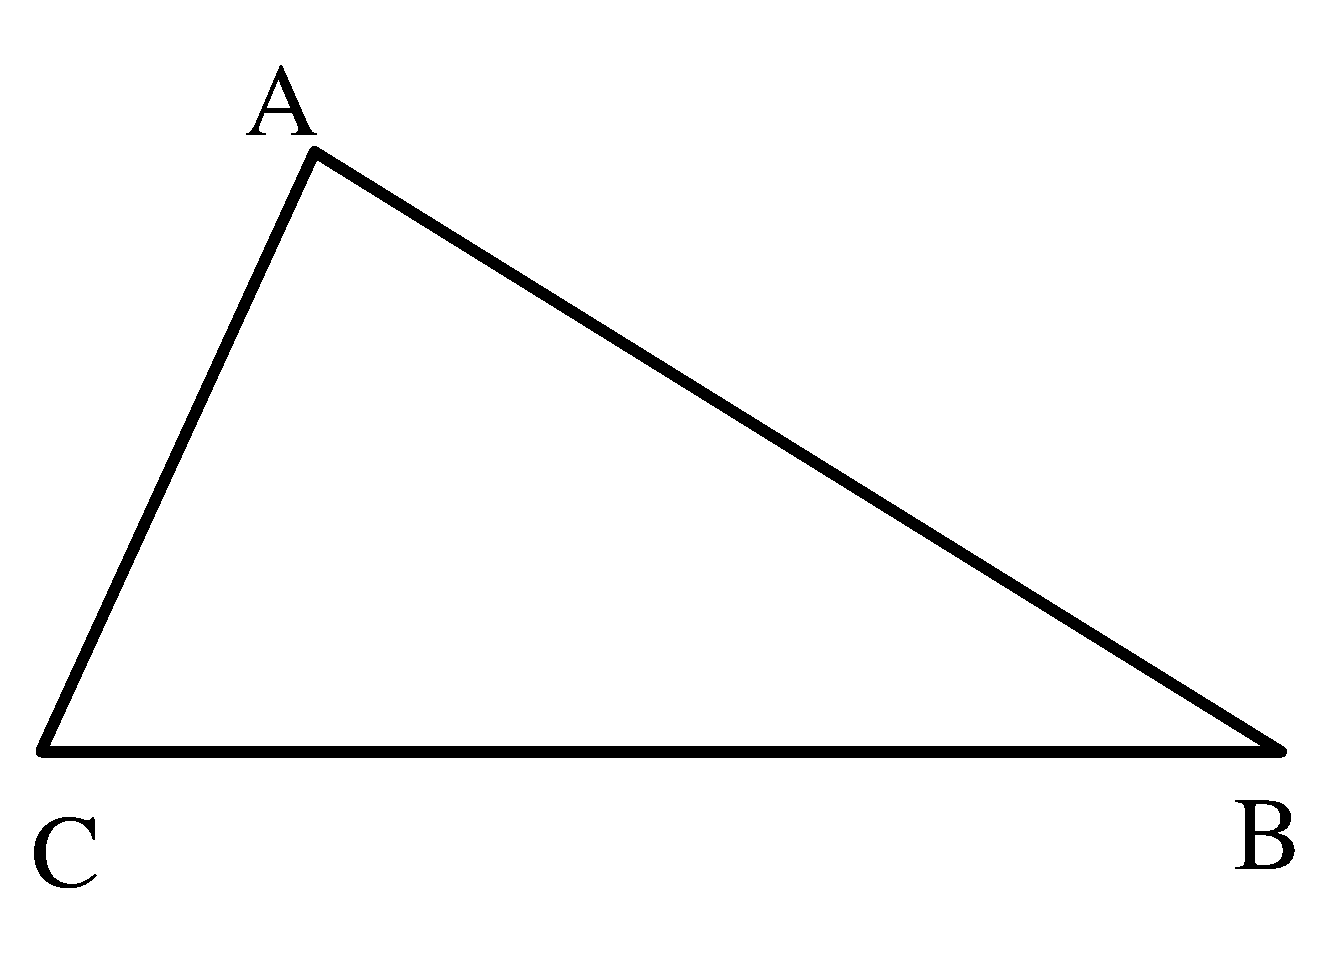
\includegraphics[keepaspectratio, width=3.0cm,height=2.4cm,clip]{eikaku_C.pdf}

                    (A) 鋭角三角形
                \end{center}
            \end{minipage}
            \begin{minipage}{0.5\hsize}
                \begin{center}
                    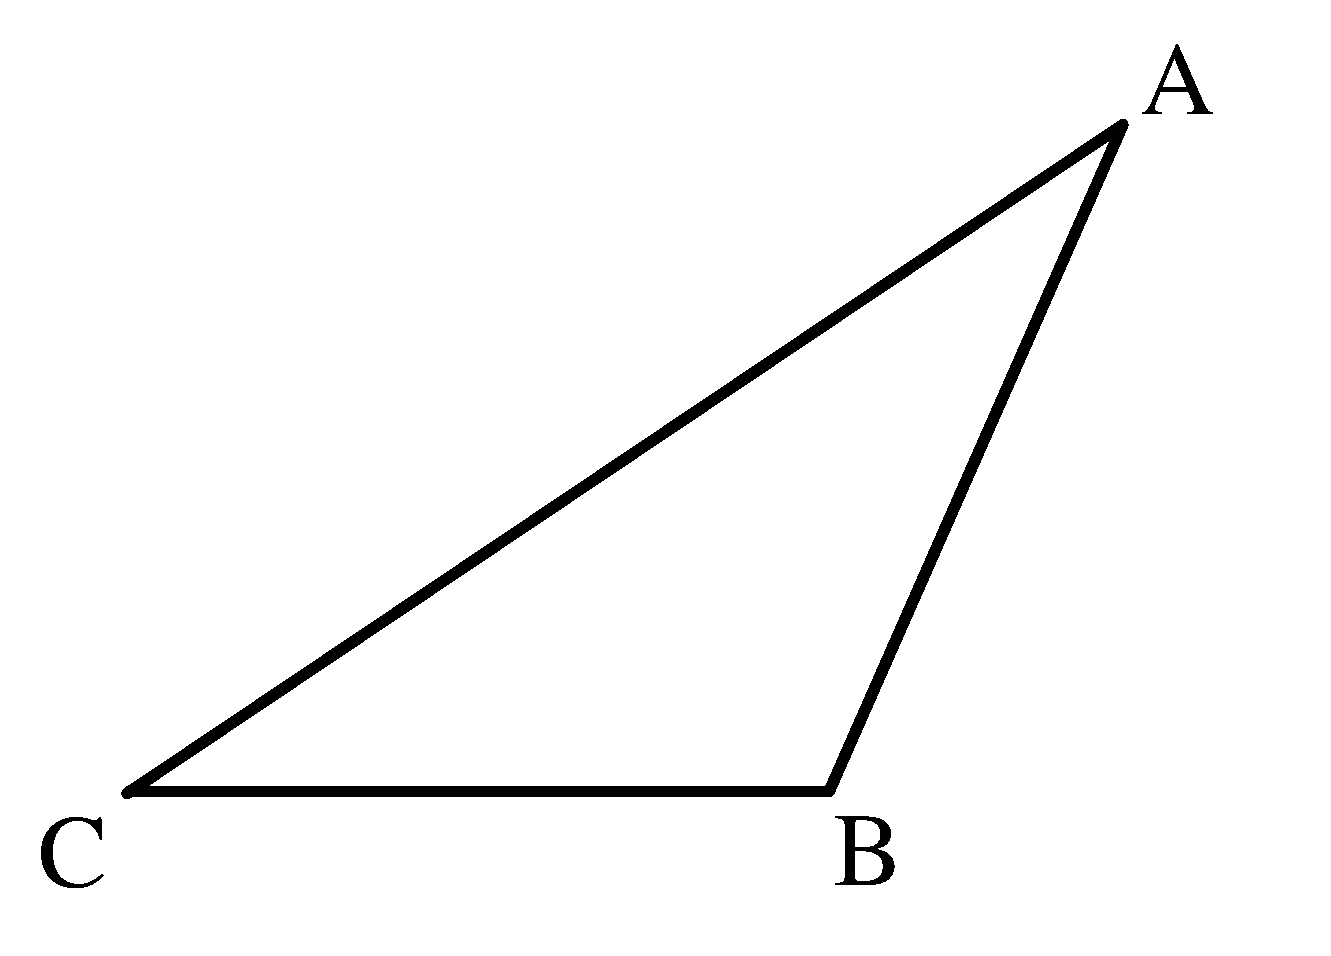
\includegraphics[keepaspectratio, width=3.0cm,height=2.4cm,clip]{donkaku_S.pdf}

                    (B) 鈍角三角形
                \end{center}
            \end{minipage}
        \end{tabular}
        \label{fig:sankakukei_no_katati}
        \caption{三角形の種類}
    \end{figure}

    ここで確認したいのは,$\sin$ 関数と $\cos$ 関数である.
    図の三角形(鋭角,鈍角のどちらでもよい)で,三角形の頂点Aから,辺BCもしくはその延長に
    対して垂線を引く.垂線の足
        \footnote{
            垂線の足:頂点Aから辺BCの延長の交点のこと.
        }
    を $H$ とする.$\angle \mathrm{ABC}$ の角度を $\theta$ と表す.
    \begin{figure}[hbt]
        \begin{tabular}{cc}
            \begin{minipage}{0.5\hsize}
            \begin{center}
                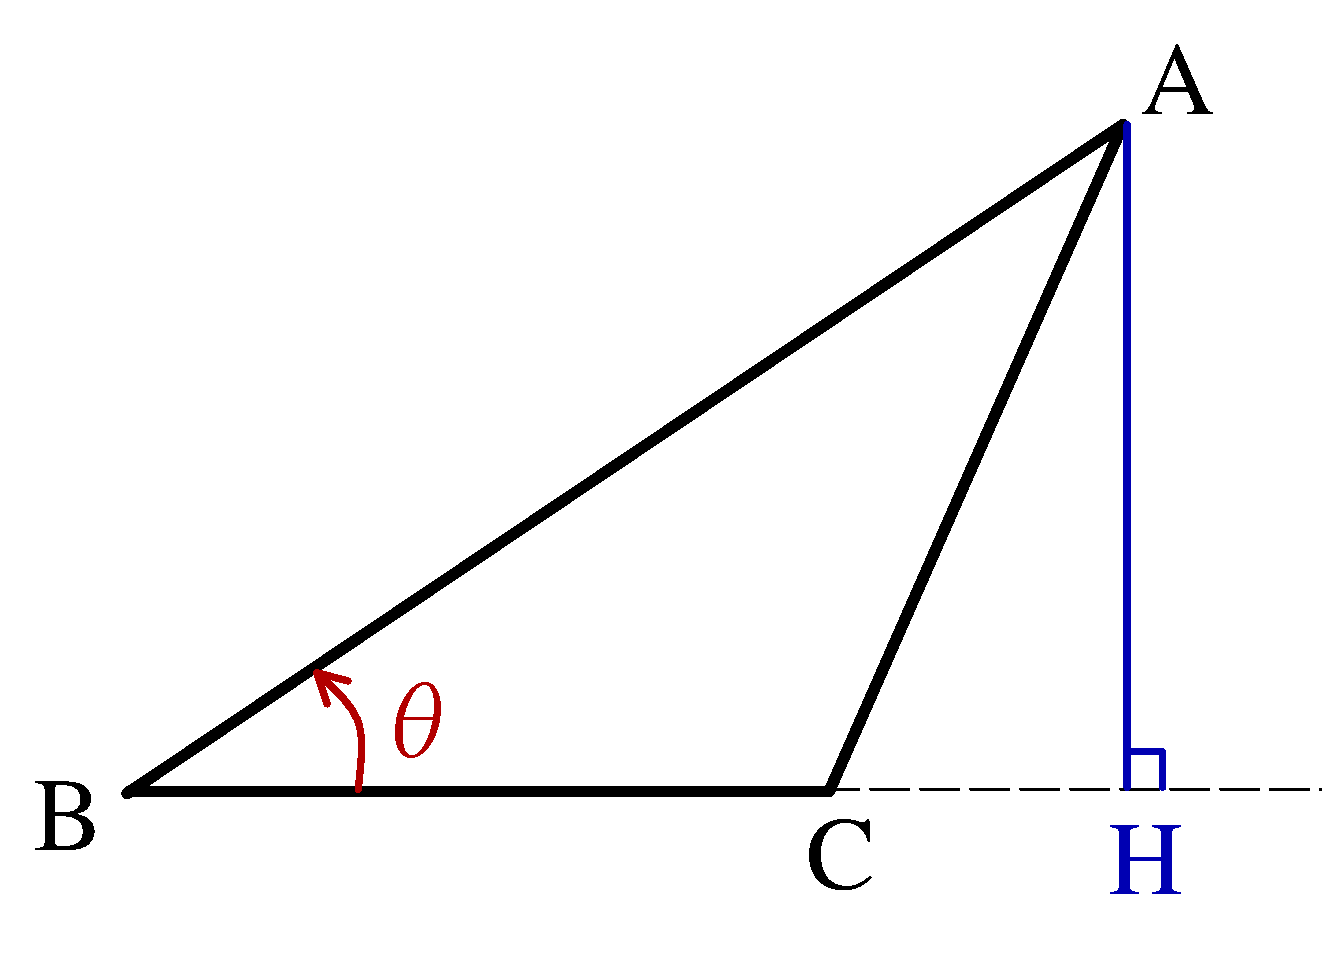
\includegraphics[keepaspectratio, width=3.5cm,height=2.8cm,clip]{function_sin_1.pdf}

                (A)
            \end{center}
            \end{minipage}
            \begin{minipage}{0.5\hsize}
            \begin{center}
                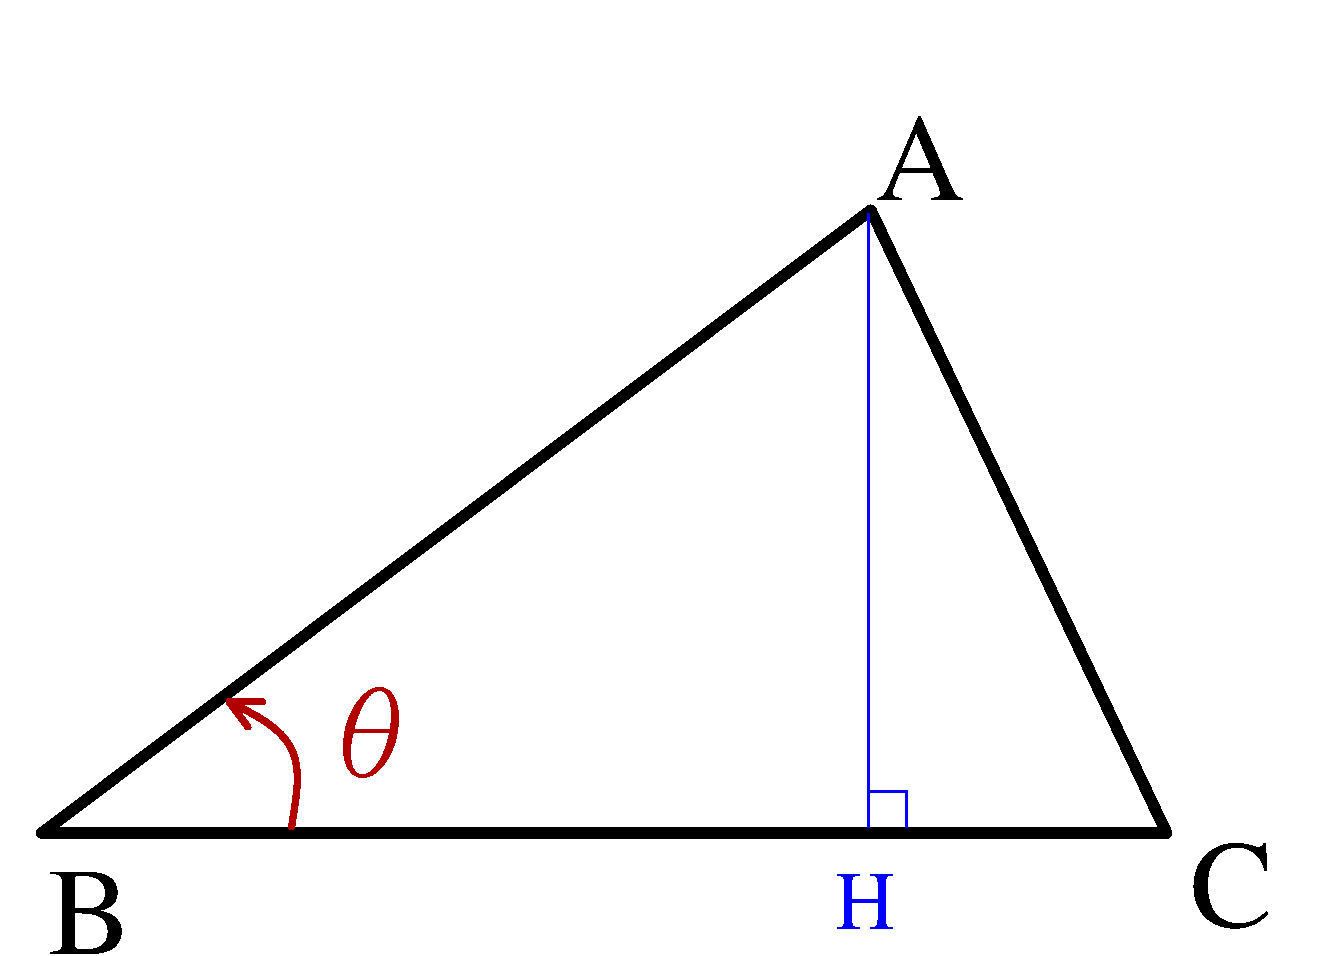
\includegraphics[keepaspectratio, width=3.5cm,height=2.8cm,clip]{function_sin_2.pdf}

                (B)
            \end{center}
            \end{minipage}
        \end{tabular}
        \caption{垂線の引き方}
        \label{fig:suisen_no_hikikata}
    \end{figure}

    これから大事なるのが,垂線AHとBHである.
    つまり,直角三角形を考えることになる.
    三角比には一般の三角形で成り立つような,
    「正弦定理」や「余弦定理」などがあるが,これらはここでは
    考えず,必要になった時に確認するという形にしたい.
    とりあえずは直角三角形を考える.

    ということで,図を以下のように書き直そう.
        \begin{figure}[hbt]
            \begin{center}
                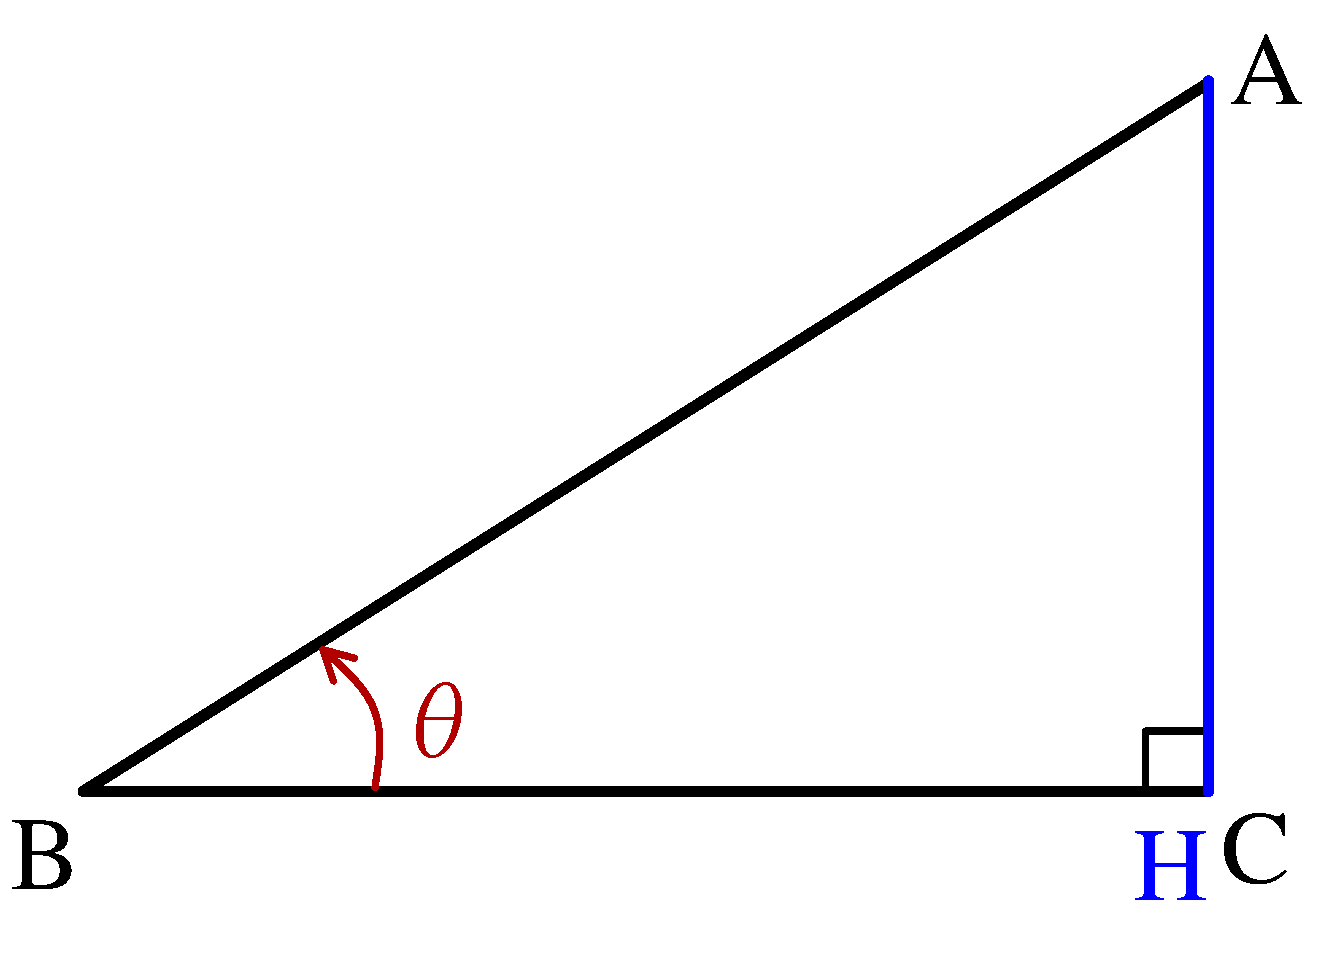
\includegraphics[keepaspectratio, width=3.5cm,height=2.8cm,clip]{sincos111.pdf}
                \caption{直角三角形の図}
                \label{fig:sincos111}
            \end{center}
        \end{figure}

    直角三角形は,辺ABの長さ $\|\mathrm{AB}\|$ と角度 $\theta$ で,その形を特定できる.
        \footnote{
            言い換えると,$\|\mathrm{AB}\|$ と $\theta$ の2つが特定されると,
            三角形の形とその大きさがきまる,ということ.
        }
    つまり,$\|\mathrm{AB}\|$ と $\theta$ がそれぞれ
    1つずつ定まれば,垂線AHの長さ $\|\mathrm{AH}\|$ が1つに定まるという関係がある.
    従って,$\|\mathrm{AH}\|$ は,$\|\mathrm{AB}\|$ と $\theta$ の関数であり,
        \begin{equation*}
            \|\mathrm{AH}\| = \|\mathrm{AB}\|\sin \theta
        \end{equation*}
    と表現する.辺ABが,基準となる水平な線よりも角度 $\theta$ だけ傾いている
    ときの,縦方向の長さが $\|\mathrm{AH}\|$ なのである.
    \begin{figure}[hbt]
        \begin{tabular}{cc}
            \begin{minipage}{0.5\hsize}
            \begin{center}
                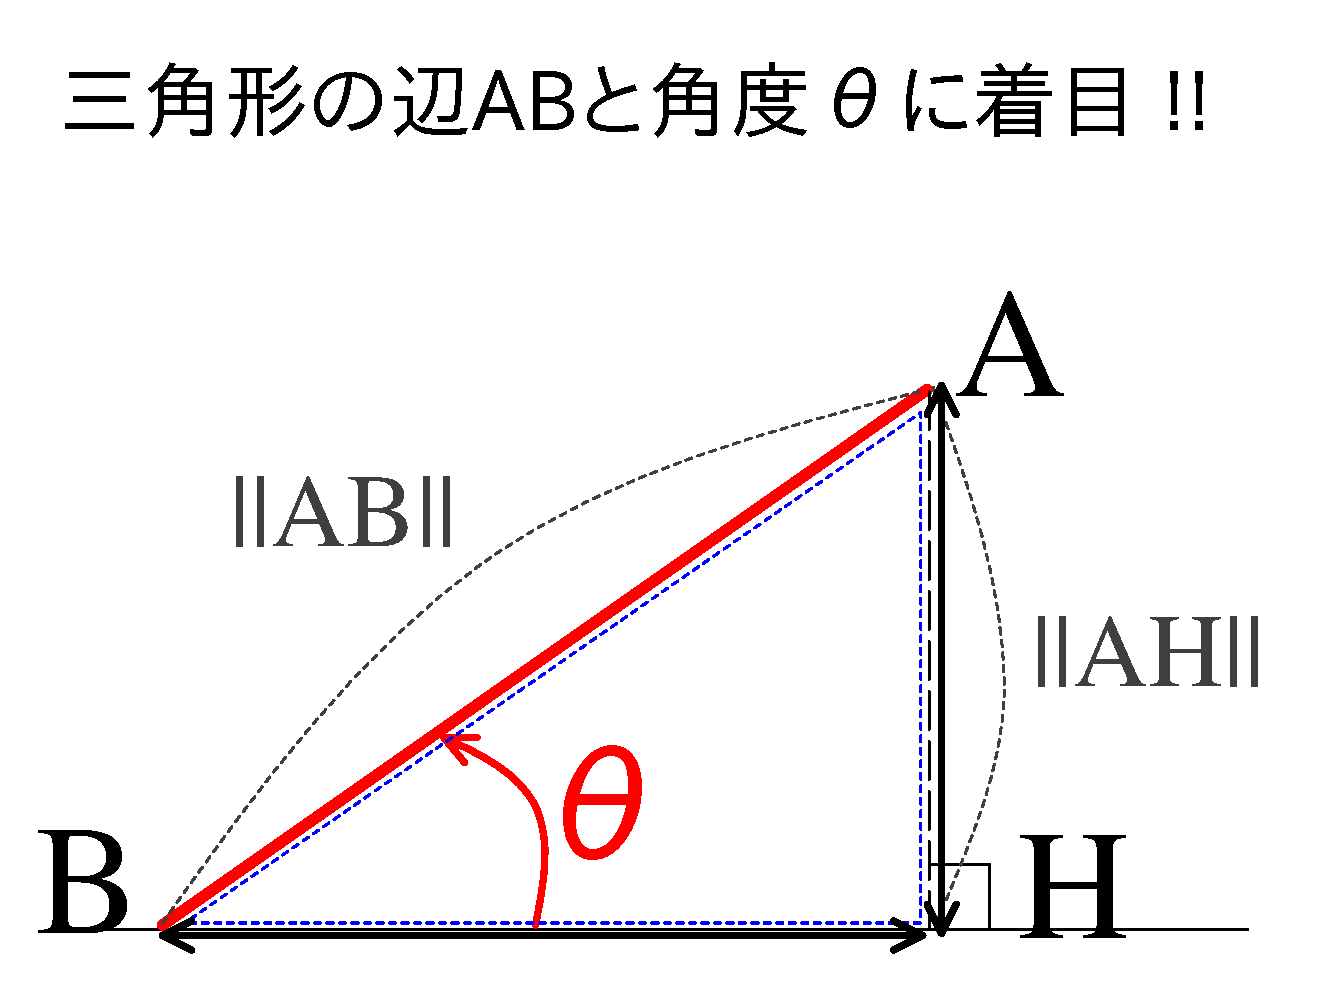
\includegraphics[keepaspectratio, width=3.5cm,height=2.8cm,clip]{sankakuhi-ABH.pdf}

                (A)
            \end{center}
            \end{minipage}
            \begin{minipage}{0.5\hsize}
            \begin{center}
                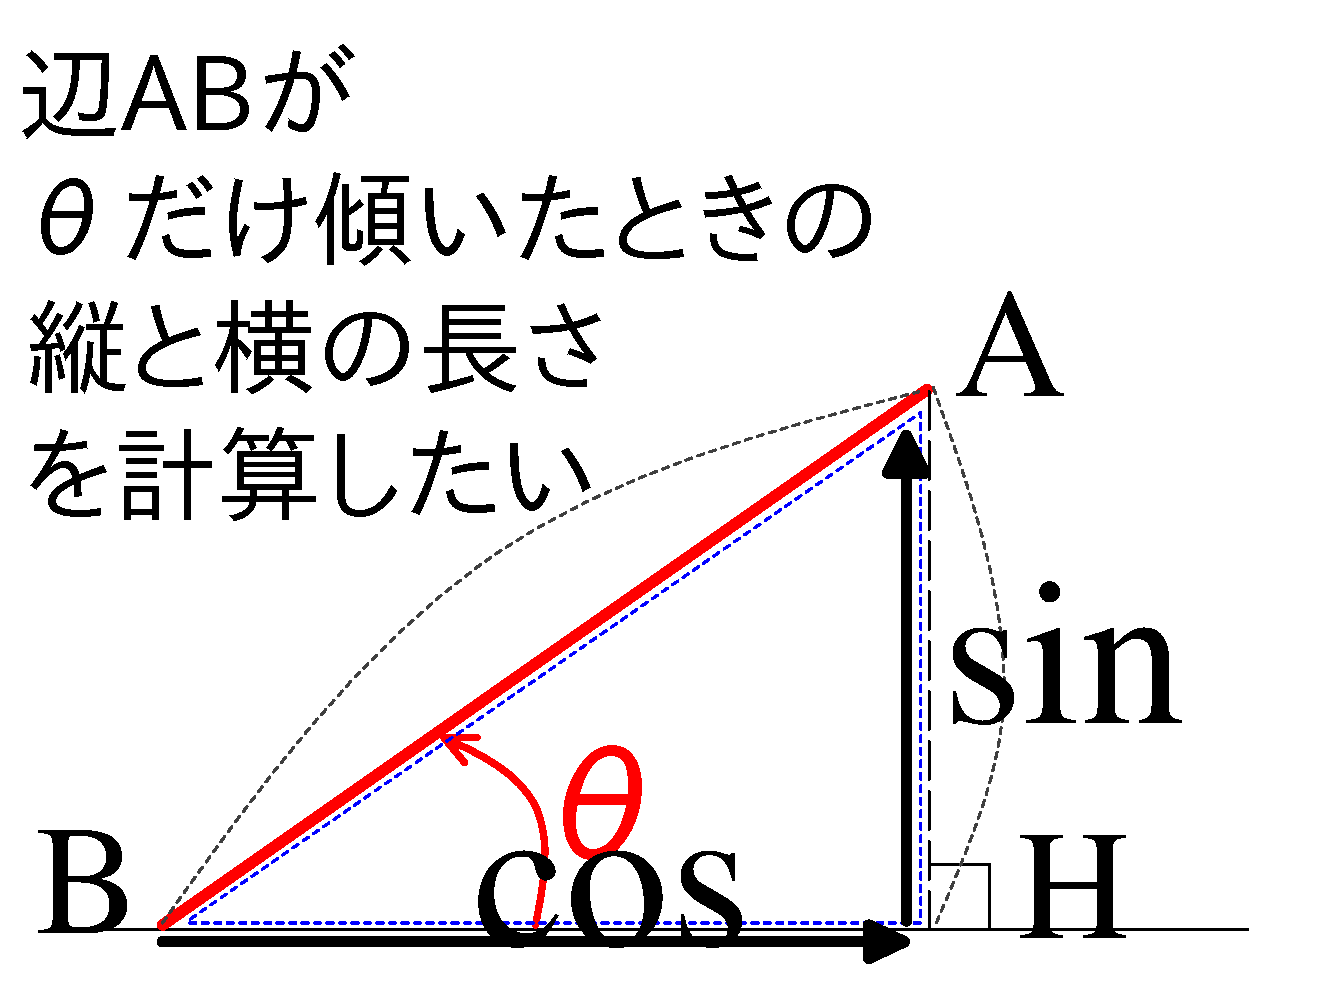
\includegraphics[keepaspectratio, width=3.5cm,height=2.8cm,clip]{sankakuhi-ABH-2.pdf}

                (B)
            \end{center}
            \end{minipage}
        \end{tabular}
        \caption{三角形の見方を変えよう}
        \label{fig:sankakukei-no-mikata}
    \end{figure}

    もう一方の辺BHの長さ $\|\mathrm{BH}\|$ も,$\|\mathrm{AB}\|$ と $\theta$ の関数である.
        \begin{equation*}
            \|\mathrm{BH}\| = \|\mathrm{AB}\|\cos \theta
        \end{equation*}
    と表現する.

    要するに,辺ABが $\theta$ だけ傾いている直角三角形の,
    縦の長さ($\|\mathrm{AH}\|$)が知りたい場合,$\|\mathrm{AB}\|$ に $\sin \theta$ を
    かけて,
        \begin{equation*}
            \|\mathrm{AH}\| = \|\mathrm{AB}\| \sin \theta
        \end{equation*}
    と計算できるということだ.横の長さ($\|\mathrm{BH}\|$)を知りたければ,$\cos \theta$ をかければよく,
        \begin{equation*}
            \|\mathrm{BH}\| = \|\mathrm{AB}\| \sin \theta
        \end{equation*}
    と計算される.$\sin \theta$ と $\cos \theta$ の値は,すでに先人が計算していて,
    今では,三角関数の表として,簡単に参照できるし,$\|\mathrm{AB}\|$ もわかる.
    つまり,三角関数を使うことで,辺ABとその傾射ている角度 $\theta$ から,
    縦と横の長さを計算で出すことができるのだ.

    さらに,$\sin \theta$ と $\cos \theta$ を使うと,
    辺ABの傾きを表現できる.一次関数,
    つまり直線の式
    では,$y=ax+b$ の $a$ が
    直線 $y$ の傾きを表している.
    傾きとは,
        \begin{equation*}
            a=\frac{(y\mbox{の増加量})}{(x\mbox{の増加量})}
        \end{equation*}
    で定義される量であった.この式の分母に $\|\mathrm{AB}\|\cos\theta$を,
    分子に $\|\mathrm{AB}\|\sin\theta$ を入れると,
        \begin{equation*}
            \frac{\sin\theta}{\cos\theta}
        \end{equation*}
    である.($\|\mathrm{AB}\|$ は約分される.)
    これは,辺ABの傾きにほかならない.これを,$\tan$ という関数記号を
    導入し,
        \begin{equation*}
            \tan\theta =\frac{\sin\theta}{\cos\theta}
        \end{equation*}
    と表現する.三角比には他にもいろいろな公式があるが,ここでは省略する.
    三角比は三角関数の特殊($0^{\circ}< \theta <180^{\circ}$)な例である.
    従って,三角比の公式は,三角関数でも成り立つ.三角関数を説明した後,
    そのうちの重要な公式を確認しよう.

    では次に,三角関数にとりかかろう.

\subsubsection{三角関数の定義}
    三角関数の定義する
        \footnote{
            この定義は,図形を用いてなされるので,
            かなり直観的で,何か受け入れがたい
            のだが,とりあえず便宜上の定義として
            考えてもらいたい.しかし,この定義は
            完全に間違っているわけではない.
            図形的に定義されるから,そこに直観が入り,
            論理が崩れてしまうという恐れがあるだけである.
            このノートでは,この図形的定義で十分である.
        }.
    図\ref{fig:sankakukansu1}を参照してほしい.
        \begin{figure}[hbt]
            \begin{center}
                \includegraphicsdefault{sankakukansu1.pdf}
                \caption{三角関数}
                \label{fig:sankakukansu1}
            \end{center}
        \end{figure}

    図を見るときに,半径 $r$ の円上を回転
    しているイメージしてほしい.この回転により,$\theta$ がいろいろな値
    に変化している様子が想像できればよい.${0\,}^{\circ} < \theta < {360\,}^{\circ}$ に
    \textbf{限らず},何回転でもできる.また,右回転(図\ref{fig:sankakukansu1}の矢印の向き)を
    正方向の回転として,その逆回転の負方向の回転も可能である.負の回転の場合,$\theta$ の取りうる
    値は負になる.この回転する半径のことを,\textbf{動径} とよぶ.\\

        \begin{itembox}[l]{三角関数の定義}
            図\ref{fig:sankakukansu1}において,三角関数 $\sin\theta$,
            $\cos\theta$,$\tan\theta$ を次で定義する.
                \begin{align}
                    \sin\theta := \frac{y}{r}\\ \notag \\
                    \cos\theta := \frac{x}{r}\\ \notag \\
                    \tan\theta := \frac{y}{x}
                \end{align}
        \end{itembox}\\
    $r$ は円の半径である.この定義では,もちろん $r  \neq  0$ と仮定している.

\subsubsection{三角関数の図形的イメージ}
    三角関数の定義式を見ても,最初はイメージしにくいここと思う.
    だから,ここで,三角関数の図形的イメージを押さえておこう.

    \begin{mysmallsec}{$\cos$ 関数のイメージ}
        最初に,$\cos$ 関数のイメージを考える.$\cos$ 関数の定義式は
            \begin{equation*}
                \cos \theta = \frac{x}{r}
            \end{equation*}
        である.但し,右辺は直交座標による.$r$ は円の半径であるから,
        定数として見てよい.例えば,$r=1$ の場合を考えてみよう.$r=1$ の
        場合,定義式により
            \begin{equation*}
                \cos \theta = x
            \end{equation*}
        となる.これは何を表しているか.式の示す通りである.
        $\cos \theta$ は $x$ の座標値に等しい.三角形で考えれば,
        半径 $r$ を斜辺とみなしたときの,$x$ 座標に等しいのである.


        半径が1でない場合はどうだろうか.その場合,定義式から,
            \begin{equation*}
                r \cos \theta = x
            \end{equation*}
        である.単に半径が1の場合の $r$ 倍になったにすぎない.


        これは,半径の $x$ 方向だけを考えたい場合に便利な道具となる.
        動径はいろいろな角度に運動するだろうが,その方向全てではなく,
        $x$ 軸方向のみを知りたい場合,その時の動径の角度を $\theta$ と
        して,$\cos \theta$ をかければよいのだ.


        長さ $r$ をもつ動径が,角度 $\theta$ の位置にあるとき,その時の
        $x$ 座標は $x = r \cos \theta$ で計算できる.半径 $r$ に $\cos \theta$ を
        かけると $x$ 座標が分かるのである.

        これはまた,\textbf{動径の $x$ 方向の長さを示している}とみても同じことである.
    \end{mysmallsec}


    \begin{mysmallsec}{$\sin$ 関数のイメージ}
        $\sin$ 関数も,$\cos$ 関数と同じように考えられる.
        $\sin$ 関数の定義は
            \begin{equation*}
                \sin \theta = \frac{y}{r}
            \end{equation*}
        である.
        半径 $r = 1$ の場合,それは動径の $y$ 座標を示す.
        $r\neq1$ の場合は,
            \begin{equation*}
                r \sin \theta = y
            \end{equation*}
        である.これは動径の $y$ 座標に他ならない.
        動径の $x$ 座標を知りたい場合は,半径に $\cos \theta$ を
        かければよいのと同様に,動径の $y$ 座標を知りたい場合は,
        $\sin \theta$ を半径 $r$ にかければよい.

        長さ $r$ をもつ動径が,角度 $\theta$ の位置にあるとき,その時の
        $y$ 座標は $y = r \sin \theta$ で計算できる.半径 $r$ に $\sin \theta$ を
        かけると $y$ 座標が分かるのである.

        これはまた,\textbf{動径の $y$ 方向の長さを示している}とみても同じことである.
    \end{mysmallsec}


    \begin{mysmallsec}{$\tan$ 関数のイメージ}
        では,$\tan$ 関数は同イメージされるのだろう.
        $\tan$ 関数の定義は
            \begin{equation*}
                \tan \theta = \frac{y}{x}
            \end{equation*}
        である.
        定義そのものを見れば,答えは意外に簡単だ.
        動径の傾きを表しているのである.これは定義式から明らかだ.動径の
        一端は常に座標のある一点から動かない.今の場合は,
        考えやすいように,座標原点に一端を固定している.だから,
            \begin{equation*}
                \frac{y}{x} = \frac{y-0}{x-0}
            \end{equation*}
        と見ることができる.動径の回転中心が座標原点ではなく,
        $(\,x_{0},\,y_{0}\,)$ の場合は
            \begin{equation*}
                \frac{y-y_{0}}{x-x_{0}}
            \end{equation*}
        である.どちらの場合も,
            \begin{equation*}
                \frac{y\mbox{の増加量}}{x\mbox{の増加量}}
            \end{equation*}
        と見ることができる.

        \textbf{$\tan$ は,動径を一次関数と見立てた時の,変化の割合を示す量}と
        見ることができる.
    \end{mysmallsec}

\subsubsection{三角関数の性質}
    三角関数には公式がいろいろとある.ここでいくつかを
    確認しておこう.

    まず,三平方の定理から,\\

        \begin{itembox}[l]{三角関数の公式}
            \begin{align}
                \sin^{2} \theta  +  \cos^{2} \theta  =  1
            \end{align}
        \end{itembox}\\
    が成立する.

    \begin{mysmallsec}{説明}
        簡単に説明する.直交座標において,
            \begin{equation*}
                x^{2}  +  y^{2}  =  r^{2}
            \end{equation*}
        が成立する.さて,この $x$,$y$ は三角関数の定義から,
            \begin{equation*}
                x  =   r \cos \theta \quad, \quad y  =  r \sin \theta
            \end{equation*}
        である.つまり,
            \begin{align*}
                x^{2}  +  y^{2}  &=  r^{2} \\
                (r \cos \theta)^{2}  +  (r \sin \theta)^{2}  &=  r^{2} \\
                r^{2} \cos^{2} \theta  +  r^{2} \sin^{2} \theta  &=  r^{2}.
            \end{align*}
        $r\neq0$ だから $r^{2} \neq 0$ であり,$r^{2}$ で割ると,
            \begin{equation*}
                \sin^{2} \theta  +  \cos^{2} \theta  =  1
            \end{equation*}
        が導かれる.
    \end{mysmallsec}




\chapter{三角関数}
    %   %-----------------------------------------------------------------------------------------------
    %   %  Input
    %   %    File Name : PhysNote_Math_DifrEq.tex
    %   %    説明      : 「微分積分学」について.考え方と使い方.
    %   %-----------------------------------------------------------------------------------------------
        %===================================================================================================
%  Chapter : 行列
%  説明    : 行列の基本的な計算規則,座標変換について
%===================================================================================================
%   %==========================================================================
%   %  Section
%   %==========================================================================
    \section{三角関数の公式}
        \subsection{加法定理}
            \begin{align}
                \sin(\alpha+\beta) &= \sin\alpha\cos\beta + \cos\alpha\sin\beta. \\
                \sin(\alpha-\beta) &= \sin\alpha\cos\beta - \cos\alpha\sin\beta. \\
                \cos(\alpha+\beta) &= \cos\alpha\cos\beta - \sin\alpha\sin\beta. \\
                \cos(\alpha-\beta) &= \cos\alpha\cos\beta + \sin\alpha\sin\beta. \\
                \tan(\alpha+\beta) &= \frac{\tan\alpha+\tan\beta}{1-\tan\alpha\tan\beta}. \\
                \tan(\alpha-\beta) &= \frac{\tan\alpha-\tan\beta}{1+\tan\alpha\tan\beta}.
            \end{align}

        \subsection{倍角公式}
            \begin{align}
                \sin2\alpha &= 2\sin\alpha\cos\beta. \\
                \tan2\alpha &= \frac{2\tan\alpha}{1-\tan^{2}\alpha}.
                \cos2\alpha &= \cos^{2}\alpha-\sin^{2}\alpha \\
                            &= 2\cos^{2}\alpha-1 \\
                            &= 1-2\sin^{2}\alpha.
            \end{align}

        \subsection{三倍角公式}
            \begin{align}
                \sin3\alpha &= -4\sin^{3}\alpha+3\sin\alpha \\
                \cos3\alpha &= 4\cos^{3}\alpha-3\cos\alpha
            \end{align}

        \subsection{半角公式}
            \begin{align}
                \sin^{2}\frac{\alpha}{2}=\frac{1-\cos\alpha}{2}. \\
                \cos^{2}\frac{\alpha}{2}=\frac{1+\cos\alpha}{2}. \\
                \tan^{2}\frac{\alpha}{2}=\frac{1-\cos\alpha}{1+\cos\alpha}.
            \end{align}

        \subsection{積和公式}
            \begin{align}
                \sin\alpha\cos\beta=\frac{\sin(\alpha+\beta)+\sin(\alpha-\beta)}{2}. \\
                \cos\alpha\cos\beta=\frac{\cos(\alpha+\beta)+\cos(\alpha-\beta)}{2}. \\
                \sin\alpha\sin\beta=\frac{\cos(\alpha+\beta)-\cos(\alpha-\beta)}{2}.
            \end{align}

        \subsection{和積公式}
            \begin{align}
                \sin{A}+\sin{B}=2 \sin\frac{A+B}{2}\cos\frac{A-B}{2}. \\
                \sin{A}-\sin{B}=2 \cos\frac{A+B}{2}\sin\frac{A-B}{2}. \\
                \cos{A}+\cos{B}=2 \cos\frac{A+B}{2}\cos\frac{A-B}{2}. \\
                \cos{A}-\cos{B}=-2 \sin\frac{A+B}{2}\sin\frac{A-B}{2}.
            \end{align}


\chapter{微分積分学}
%   %-----------------------------------------------------------------------------------------------
%   %  Input
%   %    File Name : PhysNote_Math_DifrAndIntg.tex
%   %    説明      : 「微分積分学」について.考え方と使い方.
%   %-----------------------------------------------------------------------------------------------
        %===================================================================================================
%  Chapter : 微分と積分
%  説明    : 微分積分の考え方と計算方法を確認する.
%===================================================================================================
%   %==========================================================================
%   %  Section : 極限
%   %==========================================================================
        \section{極限}
%       %----------------------------------------------------------------------
%       %  Input
%       %    File Name : PhysNote_Math_DifrAndIntg_inf.tex
%       %    説明      : 極限値:限りなく近づけるとは?
%       %----------------------------------------------------------------------
        %   %==========================================================================
%   %  Section : 極限
%   %==========================================================================
        %==================================================================
        %  SubSection
        %==================================================================
            \subsection{数列とは}

        %==================================================================
        %  SubSection
        %==================================================================
            \subsection{等差数列}

        %==================================================================
        %  SubSection
        %==================================================================
            \subsection{等比数列}

        %==================================================================
        %  SubSection
        %==================================================================
            \subsection{等比級数}

        %==================================================================
        %  SubSection
        %==================================================================
            \subsection{無限等比級数}

        %==================================================================
        %  SubSection
        %==================================================================
            \subsection{数列の極限\;\;--「限りなく0に近づける」とは --}
                微分の定義で,$\Delta x$ を「0に近づける」という表現を用いる.
                しかし,この“近づける”という表現は,どうにも,曖昧である.“
                近づける”とはいうものの,その近づける方法がよく分からないし,
                また,どの程度まで近づけられるかもはっきりとしない.そもそも,
                「近づけられるのか」という不安もある.そこで,ここでは“近づけ
                る”という作業とはどのようにすべきかを考える.まず,具体例で考
                えよう.例として,0の“次に”大きい数を考えてみよう.
                自然数で考えるならば,これは1である.しかし,
                今考えているのは,実数の範囲だから,1ではありえない.それでは
                ,0.1か.いや,もっと小さい数の0.01がある.いやいや,0.001,
                0.0001,といくらでも考えられる.この問いには,具体的に数を提示
                して,解答することはできない.それでは,「0の次に大きい数」は
                存在しないのか.0よりも少しでも大きい数は存在するが,“0の次”
                となると,答えられなくなってしまう.この問い自体が,無意味な問
                いだからである.では,なぜこのようなことを考えたかといえば,0
                の次に大きい数を考えるときに,その答えとなる数として,1,0.1,
                0.01,$\cdots$ と0にだんだんと“近づいて”いったからである.「
                近づける」という作業をしたのだ.これを,文字を用いて表現できれ
                ば,「近づける」ということを,もっと納得の行く形で受け入れるこ
                とができよう.今の手順を,もう一度詳しく,考え直そう.最初に,
                0に近い数として,1を考えた.今回は,1を考えたが,実際は0.5でも
                ,0.3でも,その他の数でも,よかった.とりあえず,考察に先立っ
                て,基準となる数を挙げただけである.そして次に最初に挙げた数よ
                りも,より小さい数を考えた.今回は1に対して0.1を挙げたが,最初
                に挙げた数の0よりも近い値であれば,どのような数でもよい.そして
                ,さらに0に近い値,もっと0に近い値へと徐々に0に近づけていった.
                この作業は無制限に続き,終わりがないが,これを自動的に行わせる
                ように,文字で表現できれば,目標を達成できる.今の例とその解答
                手順を,もう少し一般的に扱うために,文字で表現してみよう.0に近
                い数として最初に挙げる数を $a_{0}$ としよう.そして,0と $a_{0}$ の
                値との差 $\mid a_{0}-0 \mid$ を考え,これよりもさらに小さい数が
                存在するとき,そのような数を $a_{1}(<\mid a_{0}-0 \mid)$ とおこ
                う.これを繰り返すと,$a_{0}$,$a_{1}$,$a_{2}$,$a_{3}$,のよう
                な数列が得られる.この数列を $\{ a_{n} \}$ と表現すれば,$n$ が
                大きくなるに伴い,数列 $\{ a_{n} \}$ は0に近づいていくと言える.
                あとは,この作業を式で表現することを考えるのみだ.自然数 $n$ が
                大きくなるということは,「ある任意の自然数 $n_{0}$ に対して,$n>n_{0}$ と
                なるような自然数 $n$ が存在する」
                ということである.例えば,任意の自然数を,$n_{0}=100$ としてみよ
                う.この100に対して,大きい自然数は例えば200がある.そうなれば,
                $n_{0}=200$ と書き換えて,これより大きい数500を考えられる
                .さらに $n_{0}=500$ と書き換えて,$\cdots$ のように考えていけば,
                いくらでも大きな自然数を得ることができる.そして,$n$ の増加に伴
                い,$a_{n}$ と0との差が小さくなるので,その差を $\varepsilon (>0)$ と
                表現すれば,目標とする式表現として,次のように書ける.
                \\
                    \begin{itembox}[l]{限りなく0に近づける}
                        任意の正の数 $\varepsilon$ に対して,自然数 $n_{0}$ を決めることができ,
                            \begin{align}
                                n>n_{0} \quad\Rightarrow\quad \mid a_{n}-0 \mid <\varepsilon
                            \end{align}
                        が成立するならば,数列 $a_{n}$ は0に限りなく近づくと言える.
                    \end{itembox}
                    \\

                このとき,これをもっと読みやすく簡略化した式として,
                    \begin{align}
                        \lim_{n\rightarrow \infty } \{ a_{n} \} = 0
                    \end{align}
                と表現する.

                今回挙げた例の,この $\varepsilon$ に対応するのが,1である.
                この1対応して $n_{0}=1$ と決まる.そして,$n_{0}=1$ に対して,
                これより大きい自然数 $n=2$ を与えることができる.$n=2$ とした
                ときに,$\mid a_{2}-0 \mid < 1$ となるような数 $a_{2}$ が存在
                すれば,$\varepsilon$ として[1より小さい値]が存在するとして,
                $\varepsilon$ がその値で書き換えられる.今回の例では0.1である.
                また,$n_{0}=2$ とも書き換えられる.これで一巡したが,同様に,
                $n_{0}=2$ のとき,これよりも大きい自然数 $n=3$ を与えることが
                でき,$\mid a_{2}-0 \mid < 0.1$ となるような数が存在すれば,
                $\varepsilon$ をその数に書き換える.今回の例では0.01である.
                そして,$n_{0}=3$ とも書き換える.$n_{0}=3$ に対して $n=4$ が
                存在し,$\cdots$ 以下同様.

                このような作業を無制限に続けることができるとき,
                0に近づけることができるということであり,
                また,「限りなく0に近づける」という行為でもある.
                そして,この式によって,「限りなく0に近づける」
                という行為が,いわば“自動的”に行
                .「近づける」という行動を起こさなくても,極限を
                定義することができた.
                    \begin{figure}[hbt]
                        \begin{center}
                            \includegraphicsdefault{suretu_kyokugen1.pdf}
                            \caption{数列の極限}
                            \label{fig:suretu_kyokugen1}
                        \end{center}
                    \end{figure}

                また,上の例では0に近づけるということを考えたが,
                任意の実数に近づけるという作業も
                同じように考えられる.その場合,近づけたい数を $\alpha$ とするならば,
                次のように表現を拡張できる.
                    \\
                    \begin{itembox}[l]{限りなく実数 $\alpha $ に近づける}
                        任意の正の数 $\varepsilon$ に対して,自然数 $n_{0}$ を決めることができ,
                            \begin{align}
                                n>n_{0} \quad \Rightarrow \quad
                                \mid a_{n}-\alpha  \mid < \varepsilon
                            \end{align}
                        が成立するならば,数列 $a_{n}$ は $\alpha$ に限りなく近づくと言える.
                    \end{itembox}
                    \\

                このとき,これをもっと読みやすく簡略化した式として,
                    \begin{align}
                        \lim_{n\rightarrow \infty } \{ a_{n} \} = \alpha
                    \end{align}
                と表現する.


                見ての通り,先ほどの式の0を $\alpha$ で置き換えただけである.
                ちなみに,このような $\alpha $ が存在するとき,
                数列 $\{a_{n}\}$ は $\alpha$ に \textbf{収束} するという.
                また,$\alpha$ のことを数列 $\{ a_{n}\}$ の \textbf{極限} という.
                感覚的にいってしまえば,数列の項の番号 $n$ が大きくなるともなっ
                て,項の値が極限値に近づくということである.

                    \begin{figure}[hbt]
                        \begin{center}
                            \includegraphicsdefault{suretu_kyokugen2.pdf}
                           \caption{数列の極限2}
                           \label{fig:suretu_kyokugen2}
                        \end{center}
                    \end{figure}

                最初に $\varepsilon$ を設定するのは,自然数 $n_{0}$ を必ず決定できる
                ようにするためである.自然数 $n_{0}$ を決定したとしても,$\varepsilon$ は
                全く定まらない.先に $\varepsilon$ を決定しておけば,その範囲に含まれる
                自然数があるはずであり,この内のどれかが $n_{0}$ であるとして,極限の定
                義ができる.

                    \begin{figure}[hbt]
                        \begin{center}
                            \includegraphicsdefault{suretu_kyokugen3.pdf}
                            \caption{数列の極限3}
                            \label{fig:suretu_kyokugen3}
                        \end{center}
                    \end{figure}


                この定義の最大の利点は,複数の数列の極限値に関する,
                加減乗除の定理を証明できる点にある.
                例えば,2つの数列 $\{ a_{n} \}$ と $\{ b_{n} \}$ が
                あるとき,次のような数列を作ってみよう.
                    \begin{align*}
                        \{ a_{n}+b_{n} \} =
                            a_{1}+b_{1}\,,\,\,a_{2}+b_{2}\,,
                            \,\,a_{3}+b_{3}\,,
                            \,\,\cdots\,,
                            \,\,a_{n}+b_{n}\,,\,\,\cdots
                    \end{align*}
                この数列の極限はどうなるだろうか.
                これは簡単で,2つの数列 $\{ a_{n} \}$ と $\{ b_{n} \}$ の極限がそれぞれ,
                    \begin{align*}
                        \lim_{n\rightarrow \infty } \{ a_{n} \}
                            &= \alpha\, \\
                        \lim_{n \rightarrow \infty } \{ b_{n} \}
                            &= \beta
                    \end{align*}
                であるとき,数列 $\{ a_{n}+b_{n} \}$ の極限は,
                    \begin{align*}
                        \lim_{n\rightarrow \infty } \{ a_{n}+b_{n} \}
                        &= \lim_{n\rightarrow \infty } \{ a_{n} \}
                        +  \lim_{n\rightarrow \infty } \{ b_{n} \} \\
                        &= \alpha + \beta
                    \end{align*}
                となる.これを証明するには,「近づける」という表現で極限を説明し
                ただけでは論理的に不可能である.極限を式で定義することで,この定
                義に基づいて,上の公式を証明することが可能になる.


            %==================================================================
            %  SubSection
            %==================================================================
                \subsection{関数の極限\;\;-- $\varepsilon $\,-\,$\delta$ 論法 --}
                数列の極限を考えたついでに,関数の極限も考える.
                考える関数の性質として,全ての点で連続で,全ての点で微分可能な関数を考える.
                関数が連続であるとは,関数に切れ目がないことである.微分可能であるというのは,
                全ての点がなめらかにつながっているということである.

                1変数関数について考える.
                変数 $x$ をもつ関数 $f(x)$ において,ある任意の定点 $x_{0}$ を
                関数 $f(x)$ に代入する.このとき,関数が $f(x_{0})=A$ であったとする.
                つまり,関数 $f(x)$ は,点 $x_{0}$ で,$A$ という値をとると仮定しよう.

                    \begin{figure}[hbt]
                        \begin{center}
                            \includegraphicsdefault{EpDl.pdf}
                            \caption{関数の極限}
                            \label{fig:EpDl}
                        \end{center}
                    \end{figure}

                この場合,関数の極限として,1変数関数 $f(x)$ において,
                   「 変数 $x$ を限りなく $x_{0}$ に近づけると,関数 $f(x)$ の値は,
                    A に近づく.」
                と言える.しかし,これはとても曖昧な表現である.
                数列の極限で考えたときと同じように,
                この「近づける」という行為を,式で表現することにしよう.

                変数 $x$ を定点 $x_{0}$ に近づけると,関数 $f(x_{0})$ は $A$ に近づくが,
                $A$ とは一致しない.つまり,変数 $x$ を定点 $x_{0}$ に近づけているときに
                は, $A$ とは若干異なった値の $A+\varepsilon $ を示す.ここに,$\varepsilon$ は
                任意の正の定数である.$\varepsilon $ のイメージは,とても小さな値をもつ
                定数である.

                さて最初に関数 $f(x)$ に対して,$\varepsilon $ を決めると,
                これに対応して,変数 $x$ の範囲も決まる.その $x$ の範囲を $\delta $ と書こう.
                しかし,この $\delta $ が分かったとき,さらに関数 $f(x)$ が $A$ に
                近づくような範囲 $\varepsilon $ を与えなおすことができる.そうすれば,
                この $\varepsilon $ の変更に伴って,$x$ の範囲 $\delta $ も変わる.そ
                うなれば,変更された $\delta $ に対して,さらに $f(x)$  が $A$ に
                近づくような範囲に $\cdots$.これは無制限に続けることができ,最終的に
                は,関数の極限として,$x$ を $x_{0}$ に近づけたときに,$A$ の値を得る,
                ということになる.

                このように,最初の一回だけ $\varepsilon$ を指定するだけで,
                あとは無制限に自動的に,関数の極限値を得られる.以上をもう
                少し詳しく記述し,式で表現して見よう.

                関数 $f(x)$ において,変数 $x$ を $x_{0}$ に近づけるが,
                $x_{0}$ に一致させないようにするとき,
                $\mid x-x_{0} \mid$ はある正の値 $\delta$ をもつ.
                この $\delta$ のイメージは,$x_{0}$ を
                含むような,変数 $x$ の微小な区間である.
                そして,関数 $f(x)$ には,この微小区間 $\delta$ に対応して,
                $\mid f(x) - A \mid$ という正の値 $\varepsilon$ という値域
                をもつことになる.$f(x_{0})=A$ であるので,$\varepsilon$ が
                より小さくなれば,さらに関数は $A$ からの範囲を狭めていくこ
                とになる.関数 $f(x)$ は連続な関数なので,$\varepsilon$ をさ
                らに小さくすることは可能である.$\varepsilon$ をさらに小さく
                するに伴い,$\delta$ もさらに小さくなっていく.
                もちろん,$\delta$ をいくら小さくしても,その範囲の中には $x_{0}$ が
                含まれている.

                式で書いてみよう.まず,$A$ からのずれの程度の指標である,
                $\varepsilon$ が考えられる.そして,この $\varepsilon$ が
                定まることで,$x$ の範囲もきまり,$\delta$ となるとき,
                    \begin{align}
                        \mid x-x_{0} \mid < \delta \quad
                        \Rightarrow \quad \mid f(x) - A \mid < \varepsilon
                    \end{align}
                であるならば,関数 $f(x)$ は,変数 $x$ を定点 $x_{0}$ に
                近づけたときに,$A$ に収束すると言える.

                今までは連続関数を考えてきたが,実際は,もう少し制限を緩めることができる.
                というのも,関数 $f(x)$ は区間 $I$ のみで連続と定義されていればよく,
                また一方で,$x$ も $x_{0}$ の点で定義されていなくてもかまわない.
                $f(x_{0})$ が定義されていなくても,$x$ は単に $x_{0}$ に近づけるだけ
                であり,一致させるわけではないので,不都合は生じない.

                最初に $\varepsilon$ の存在を確認したのは,このためである.
                もし $\delta$ の存在を先に認めてしまうと,もしかしたら,
                関数が定義されないような範囲を選んでしまう可能性がある.
                そうなれば,上の式は,その関数が定義されていない点に差し掛かったとき,
                極限が存在しないという結論を出してしまう.



%   %==========================================================================
%   %  Section : 積分
%   %==========================================================================
        \section{積分}
%       %----------------------------------------------------------------------
%       %  Input
%       %    File Name : PhysNote_Math_DifrAndIntg_intg.tex
%       %    説明      : 積分学を確認する.
%       %----------------------------------------------------------------------
        %   %==========================================================================
%   %  Section : 積分
%   %==========================================================================
        %==================================================================
        %  SubSection
        %==================================================================
            \subsection{面積は積分によって定義される}
                面積の定義は「縦$\times$横」であるが,この定義は図形ありきのものである.
                しかし,数学的に面積を議論したい場合には,不十分である.面積の数学的
                定義は積分によって定義されるべきである.以下では,積分について考えていこう.
                
                積分を勉強する前に,大事な注意をしておきたい.議論の最初から「面積」という
                言葉を定義なしに使用する.定義なしの「面積」はイメージとして捉えてほしい.
                面積は積分によって定義したいので,積分を定義するのに面積は使ってはいけない
                    \footnote{
                       もし,積分を面積によって定義してしまったら,論理的不整合になる.
                       循環論法になってしまうのだ.
                       積分の定義に面積が必要で,その面積の定義には積分が必要となってしまっては
                       数学的議論が循環してしまう.公理から定義や証明によって演繹的に構築される
                       数学としてこれは絶対に避けるべき.
                    }. 
                そうかと言って,面積のイメージなしに積分を説明するのは困難である.
                では,どうするか.無駄のない論理を構築したい場合は,面積という語彙を使わずに
                単なる計算として積分を定義したあとに,この積分によって面積を説明すべきであろう.
                しかし,これではイメージがしにくく学習効率がわるい.だから,このノートでは
                妥協して,積分の説明に「面積」という語彙を使用する.ただし,積分を定義する前に使用する
                「面積」はあくまでも日常言語的なイメージであり,数学的概念ではない.

                面積の定義をしなくても積分を定義できる.だけど,「面積」のイメージなしに
                積分の定義を理解することは困難である.だから,積分の定義を説明するのに「面積」という
                語彙を使用する.積分が定義できた暁には,それまで使用した「面積」のイメージを
                一切擦れたふりをしよう.積分の定義は単なる計算であり,「面積」の概念は使われていない.
                積分の定義を理解するのに使用する「面積」は補助輪である.積分が理解できたら,補助輪を
                外そう.そして,積分によって補助輪(「面積」)を定義するのだ.

        
        =================================================================
        %  SubSection
        %==================================================================
            \subsection{長方形の面積公式に対する疑問}
                積分は面積と深くかかわりがある.そこで,ここで改めて,
                面積とは何かを考えてみる.

                目標は任意の一変数関数 $f(x)$ の積分を定義することだ.
                以下,変数 $x$ は $f(x)$ の独立変数であり,実数であるとする.

                面積といえば,最
                も基本的な面積公式として,長方形の面積の公式
                    \begin{equation*}
                        \mbox{縦} \times \mbox{横}
                    \end{equation*}
                がある.
                    \begin{figure}[hbt]
                        \begin{center}
                            \includegraphicslarge{ChouhoukeiMenseki.pdf}
                            \caption{長方形の面積}
                            \label{fig:ChouhoukeiMenseki}
                        \end{center}
                    \end{figure}

                長方形の面積というものを,小学校でどのように教わったか忘れてしまったが,
                おそらく,天下り的に教わったのではないかと思う.しかし,強引に押し付けられた
                この式を,単純に鵜呑みにするには少々抵抗がある.
                そこで次節から,改めて長方形の面積はなぜ「縦の長さ$\times$横の長さ」なのかを,
                できるだけ,合理的に説明してみよう.

        %==================================================================
        %  SubSection
        %==================================================================
            \subsection{長さとは何か}
                まず,長さという概念を考えないといけない.これは何も難しく考えることない.
                なぜなら,私たちは定規を使って長さを測るという行為をすでに会得しているから
                である.少し畏まった形で,説明してみよう.

                長さは,数直線状の2点の間の距離として捉えれば良い.
                    \begin{figure}[hbt]
                        \begin{center}
                            \includegraphicsdefault{NagasaToSuuchokusen.pdf}
                            \caption{棒の長さと数直線}
                            \label{fig:NagasaToSuuchokusen}
                        \end{center}
                    \end{figure}

                棒の長さ $l$ を考えるなら,棒を数直線に並べて置いて,棒の両端に
                対応する数直線上の2点 $a$,$b$ ($a<b$ となるように置く)から,
                    \begin{equation*}
                        l = b - a
                    \end{equation*}
                とすれば,長さを数で表せる.

                さらに言えば,棒を置く位置は
                どでもよいから
                    \footnote{
                        棒を置く位置によって,棒の長さが変わることがないという
                        前提の上での話である.
                    },
                棒の一端を数直線上の原点,つまり,数値0に対応するようにして,
                さらに,もう一端を正の数値 $x(>0)$に対応するように置ける.
                    \begin{figure}[hbt]
                        \begin{center}
                            \includegraphicsdefault{NagasaToSuuchokusen_0.pdf}
                            \caption{棒の長さ}
                            \label{fig:NagasaToSuuchokusen_0}
                        \end{center}
                    \end{figure}

                すると,
                    \begin{equation*}
                        l = x - 0 = x
                    \end{equation*}
                となる.$l=x$ となって,数値 $x$ がそのまま棒の長を示すことになる.

                なんだか面倒な言い回しになってしまったが,要は,
                棒の長を測るには,棒の端に定規の0をあてて,
                もう一方の端に対応する数値 $x$ を読めば,
                この数値 $x$ が知りたかった棒の長さ $l$ と
                同一視できるということである.単に,定規を使って
                棒の長さを測るという行為を,式を使って丁寧に説明
                しただけだ.

        %==================================================================
        %  SubSection
        %==================================================================
            \subsection{長方形の面積とは何か}\label{sunsec:ChouhoukeiNoMensekiToha}
                長さは,数直線上の点により表現できることがわかった.では,
                面積はどうだろうか.たしかに,私たちは長さという概念だけで
                はなく,平面的な広がりというものも感じ取ることができる.そ
                して,様々な広がりの大きさを感じてもいる.例えば,土地の広
                さが良い例だ.土地を持っていると,国に税を払わないといけな
                いが,この税の支払い額は所有している土地の広さに大きく影響
                する.当然,広い土地を持っているほど,多額の税金を国に収め
                ないとならない.現実には,土地の面積でけで税の支払い額が決
                まるわけではないが,ここでは,話を単純にするため,面積のみ
                で支払う税金の額が決まるとしよう.つまり,同じ大きさの土地
                を持っている者は,同額の税を払うことになる.こうなると問題
                になるのが,土地の大きさの測り方である.どうやって,土地の
                広さが同じだとか,どちらが小さいとかをきめれば良いのだろう
                か.もし,正確に表すことができなければ,例えば,同じくらい
                の広さの土地を持つものが二人いたとして,支払う税額が両者で
                異なれば,争いが起こることは必至である.幸いにも,この問題
                を解決するすべを,すでに私たちは持っている.面積という概念
                が,その解決の鍵だ.ある決まった広さを基準として,その何倍
                かで広さを表すのである.これにより,広さを数量的に比較する
                ことができるのである
                    \footnote{
                        実際には,面積の測定方法はどうするかといった問題が
                        ある.同じ土地の面積を測るのに,毎回異なる結果を出
                        すような測定方法ではダメだ.かなり深刻な問題だけど
                        ,ここで無視しよう.
                    }.

                長さが数直線状の2点で表すことができたなら,面積も同じように
                考えることができないだろうか.全く同じように考えることはでき
                ないが,この考え方を真似ることはできる.数直線を2つ使うのである.
                    \begin{figure}[hbt]
                        \begin{center}
                            \includegraphicslarge{Menseki00.pdf}
                            \caption{面積}
                            \label{fig:Menseki00}
                        \end{center}
                    \end{figure}

                2つの数直線を用意し
                    \footnote{
                        この2つの数直線の目盛の間隔の長さは,
                        実のところ異なっていてもよいが,ここでは考えやすいように,
                        目盛の間隔は同じであるとしよう.
                    },
                直角に交わるようにする.このような行為を,2つの
                直線を \textbf{直交} させるといい,また,
                この2つの直線は直交しているという.
                考えやすいように,両数直線ともに,原点で直交させよう.

                2つの数直線が直交している部分の近くに,長方形を置く.
                置き方はいろいろ考えられるが,長方形の辺が用意した数直線
                に平行になるようにしよう.すると,各辺の頂点を数直線上の
                数値に対応するようになる.つまり,辺の長さが数によって表現
                できるのである.

                長方形のもつ辺はの数は,縦2本と横2本で,合わせて4つだが,
                縦と横の2本づつの辺の長さは同じである.つまり,
                長方形の形を明確にするには,縦1個と横1個の2つの辺の長さが
                分かれば良い.縦の長さを $m$,横の長さを $l$ とおく.
                縦の長さ $m$ は,辺の頂点が数直線上の $a$,$b$ に対応
                しているとき($a<b$ となるようにする),
                    \begin{equation*}
                        m = b - a
                    \end{equation*}
                である.横方向の長さについても同じように考えて
                ($c<d$ となるようにする),
                    \begin{equation*}
                        l = d - c.
                    \end{equation*}
                長方形の面積はこの2つの長さ $l$,$m$ によって,確定する.
                長方形の面積を表す記号を,$S_{\mbox{\small{長方形}}}$ としたとき,
                $S_{\mbox{\small{長方形}}}$ は $l$ と $m$ を用いて,
                    \begin{equation*}
                        S_{\mbox{\small{長方形}}} = l \times m
                    \end{equation*}
                と定義される.
                これは数直線上の数値 $a$,$b$,$c$,$d$ で表せば,
                    \begin{equation*}
                        S_{\mbox{\small{長方形}}} = l \times m = (d-c) \times (b-a)
                    \end{equation*}
                となり,ひとつの数値に確定する.

                面積とは,2つの独立した数直線上にある,それぞれの区間の長さ $l$,$m$ に
                よって特徴付けられるものである.
                小学校では,「長方形の面積は縦$\times$横である」と
                押し付けられるように教わったが,縦や横とはなんのことかはそれほど明確
                には説明されていなかった.ここでは,縦と横を直交する2つの数直線である
                ように,置き換えることで明確にすることができた.

                しかし,面積は,なぜ,乗算で定義されているのだろうか.加算で定義しても
                よさそうではないか.また,少々おかしいかもしれないが,減算や除算で
                も,論理的に矛盾することのないように,面積を定義することもできるの
                ではないか.もしかしたら,予想通り
                    \footnote{
                        確かめてないからわかりません.もしかしたら,簡単に否定されて
                        しまうかもしれない.
                    },
                乗算以外でも定義可能かもしれない.しかし,広さを数で表すのに最も
                直感と合うものは,掛け算である.例えば,横の長さが1だけ増えるとしても,
                長方形には縦の長さもあるから,その分だけ余計に面積が増える.
                式で書けば,もともと面積が $S_{\mbox{\small{長方形}}}=l\times m$ で
                あった場合に,$l$ が1増えるとで,
                    \begin{equation*}
                        S_{\mbox{\small{長方形}}} = \left( l+1 \right) \times m
                                                  = l \times m + m
                    \end{equation*}
                となって,たとえ $l$ が1しか増えなかっとしても,面積は $m$ だけ
                増えることになるのである.縦横にぎっしりと詰めたタイルを,さらに
                横にその数を増やすときには,縦の枚数分だけのタイルが必要になるの
                である.乗算による定義はこのイメージと一致するのだ.
                    \begin{figure}[hbt]
                        \begin{center}
                            \includegraphicslarge{MensekiToKakezan.pdf}
                            \caption{面積はなぜ掛け算で定義されるか}
                            \label{fig:MensekiToKakezan}
                        \end{center}
                    \end{figure}

            \begin{memo}{一般的な形の面積}
                ちょっと関係ないことになるが,ついでに任意の図形の
                面積について考えてみよう.

                たしか,小学校では,一般的な形の面積を測る方法
                として,基準となる面積が1のタイルを持ってきて,
                その任意の形にを覆うのにひつようなタイルの枚数を
                数える,ということをしたはず.この考え方は,とても
                大切な考え方である.とても素朴で,それこそ,小学生でも
                理解できるのだけど,すごく重要なことを含んでいる.

                もちろん,ここで用意した
                タイルは同じ形のものなので,任意の形をした図形に対して
                ぴったりと覆うことはできず,足りない部分や,はみ出してしまう
                部分も生じる.小学校では,「だいたいこのくらい」で終わってし
                まっただろうが,この考え方をもう一段階進めてみると,任意の形
                をした図形の面積を正確に表現できるようになる.その一段階は
                案外に低い.とても小さいタイルを用意すれば良いのである.
                タイルが小さいほど,隙間を詰めやすくなり,タイルの覆う面積が
                本来の任意の図形の面積に近づく.
                \begin{figure}[hbt]
                    \begin{tabular}{cc}
                        \begin{minipage}{0.5\hsize}
                            \begin{center}
                                \includegraphicsdouble{MensekiToZahyou.pdf}

                                (A)
                            \end{center}
                        \end{minipage}
                        \begin{minipage}{0.5\hsize}
                            \begin{center}
                                \includegraphicsdouble{MensekiToZahyou_dtl.pdf}

                                (B)
                            \end{center}
                        \end{minipage}
                    \end{tabular}
                    \caption{面積}
                \end{figure}


                この考え方は,微分積分学の心に直結する大切な精神を含んでいるので,
                もう一度,繰り返しておこう.直感的に分かりきっていることだけど,
                大変大切な考え方である.

                任意の大きさの長方形を1つ用意して,この1つを複製する.
                用意した長方形の面積は,すでに知っているとする.それで,
                複製した長方形を,面積を知りたい図形の内側に,できる限り稠密
                    \footnote{
                        稠密:隙間なく,ぎっしりと詰まっている様子を,\textbf{稠密} で
                        あるという.ここで使った「できる限り稠密」の意味は,本来の「稠密」の意味
                        からずれているが,隙間の面積が最小になるようにという意味で,「できる限り稠密」
                        という表現を使った.
                    }
                になるように並べる.そして,任意の図形の面積を,並べたすべての長方形の
                面積の合計で近似するのである.もちろん,隙間の文だけの誤差は生じる.
                この誤差が気になるようだったら,はじめに用意する任意の大きさの長方形を
                より小さいものにすれば,それだけ隙間を埋めることができ,その誤差を小さ
                くできる.

                ここで,誤差を「小さく」できると言ってしまった.
                この言い方では,どれだけ誤差を
                小さくできるのかが不明確で,曖昧さを含んでしまう.
                この曖昧さを解消するために厳密には,$\varepsilon - \delta$ 論法を
                使うのであるが,物理学を学ぶ上では,このような厳密さにはそんなにこだわる
                必要はないので,ここでは少々細かいことには目をつぶって,先に話を
                進めていこう
                    \footnote{
                        ただし,もちろん,一度も厳密に考えないというはよくない.
                        暇なときに,物理学を学ぶのに飽きたときに,数学の教科書を
                        読んでおくべきだ.ここで厳密さを無視したのは,あくまでも
                        物理学を行う上では無視しても支障がないからであり,重要で
                        ないからということではない.
                    }.
            \end{memo}

            \begin{memo}{「直角」とは何か}
                2つの直線が「直交する」ということは,
                その2つの直線が直角に交わっていることであると,
                上に記述した.では,「直角」とはなんだろうか.
                交わる角度が $\pi/2$(度数表記では90${}^{\circ}$)で
                ある場合に,直角に交わっていると表現する.
                この説明に従うと,$\pi/2$ は
                円の一周する角度 $2\pi$ の$1/4$ だから,その円の
                2つの直径が円を4等分する角度で交わっている,
                と言うことになる.何が4等分なのかといえば,それは円の
                面積に他ならない.
                    \begin{figure}[hbt]
                        \begin{center}
                            \includegraphicslarge{ChokkakuTohaNanika00.pdf}
                            \caption{円の面積と直交する2つの直線}
                            \label{fig:ChokkakuTohaNanika00}
                        \end{center}
                    \end{figure}

                となると,直角を説明するより先に,面積について説明すべき
                である.しかし,上に説明した考え方に従うと,円の面積を知るには,
                無限に小さな長方形でその円を覆わないとならない.
                そして,ひとつの長方形の面積は,
                上の記述
                    \footnote{
                        \ref{sunsec:ChouhoukeiNoMensekiToha}節参照.
                    }
                によれば,直交する2つの直線という概念を元に,
                説明されるものである.

                さて,語彙の説明の循環に気づいただろうか.直角を説明する前に,面積について
                説明しようとしたのだけど,その面積の説明をするのに,直角という考え方を
                使ってしまったのである.つまり,この説明では,面積と直角の両方の語彙について,
                説明がなされていないということである.

                では,上の説明のどこに間違いがあったのか.答えは簡単だ.「直角に交わる」ということを,
                視覚的な直感に頼ってしまったことである.なぜだか知らないが,人間の目には,「直角」が
                他の角度よりも特別な角度であると,感じてしまう.この感覚が,このような間違いを起こした
                と考えてよいだろう.つまり,より大げさに言うなら,図形の性質の視覚に頼った説明は,
                論理に矛盾を生じやすいということである.

                そうなると,どう正せばよいかということに関心が向かうが,一番手っ取り早い方法が,
                後に説明することになる,\textbf{ベクトルの内積$\cdot$外積} という概念を使うこと
                である.どういう事かといえば,
                「ある条件式
                        \footnote{
                            先走って,書いておくと,2つのベクトル $\ba$,$\bb$ があるとき
                            (ただし,$\ba$,$\bb$ ともに零ベクトルでないとする),
                            $\ba\cdot\bb=0$ であるならば,$\ba$ と $\bb$ は \textbf{直交} していると
                            いう.「ベクトル」という単語を,「直線」と置き換えることで,
                            2つの直線が直交する条件を得ることができる.

                            詳細は,
                            \ref{subsec:VecNaisekiFig}節(\pageref{subsec:VecNaisekiFig}ページ),
                            \ref{subsec:VecNaisekiArg}節(\pageref{subsec:VecNaisekiArg}ページ),
                            \ref{subsec:VecNaisekiStt}節(\pageref{subsec:VecNaisekiStt}ページ),
                            \ref{subsec:VecGaiseki}節(\pageref{subsec:VecGaiseki}ページ)を参照.
                        }
                が成り立つとき,そして,その場合に限り,2つの直線は直交しているという」
                といった,説明になるのだ.

                言いたかったことは,\textbf{上記の説明には,矛盾点が含まれる}ということであり,
                この点に注意してほしい,ということである.直感的に説明しようとしたばっかりに,
                このような矛盾した記述を行ってしまった.
                さらに白状すれば,このノートでは,多かれ少なかれ,この種の矛盾した
                説明を行ってしまうこととなる.しかし,このような矛盾した説明は,
                物理学を直感的に説明しようとする場合には,回避ができないと思われる
                    \footnote{
                        少なくとも,私には,物理学を論理的に矛盾なく説明するだけの力はないし,
                        それがこのノートの目的ではない.このノートの目的の一つは,自然界の現象を
                        物理学を通して,ごく直感的にみることである.
                    }
                なので,このノートを読む場合には,少々矛盾した説明にめをつむっていてもらいたい.
                また,矛盾しているか否か意識しながら,読み進めてもらいたい.
            \end{memo}

        %==================================================================
        %  SubSection
        %==================================================================
            \subsection{関数と,図形の面積}
                長方形の面積について,改めて考え直した.そして,一般の図形の
                面積の求め方の考え方も紹介した.そして,いよいよ,次に積分の
                定義にとりかかるのであるが,いきなり定義を紹介したところで,
                意味不明で消化不良を起こしかねない.なので,少しずつ段階を踏んで,帰納
                的
                    \footnote{
                        帰納的:具体例から一般的に通用する表現を得ることを,
                        「\textbf{帰納的} な手段で,一般規則を得る」などという.
                        学問は,主として,帰納的な考え方によって理論が組み立て
                        られる.なぜなら,世の中には具体例しか存在しないからで
                        ある.具体例の共通点を洗い出して,より一般に通用する規則
                        を見つけるのである.それが数学では公理であったり,物理学で
                        は法則と言われたりするものである.
                    }
                に積分の定義について考える.

                目標は,一般の図形の面積が計算できるようになること,である.
                しかし,いきなり一般の図形を考えることは難しいので
                    \footnote{
                        少なくとも,私にとっては,難しいです.
                    },
                まずは,以下のような状況を考える.一般の図形の面積を
                考えるには,図\ref{fig:IntegFuncKangaeKata00}のように考えると良い.
                    \begin{figure}[hbt]
                        \begin{center}
                            \includegraphicslarge{IntegFuncKangaeKata00.pdf}
                            \caption{$S$ は関数 $f(x)$ と $g(x)$ の間の面積とみなせる}
                            \label{fig:IntegFuncKangaeKata00}
                        \end{center}
                    \end{figure}

                まず,面積を知りたい図形があり,その面積が仮に計算可能であったとして,
                その面積を $S$ としよう.面積 $S$ を知る方法として,まず,図形の縁
                    \footnote{
                        縁:「ふち」と読んでください.「えん」ではありません.
                        図形の周囲を囲む縁のことを言っているんです.
                    }
                に着目する.どうするかというと,この図形の縁を上下に分けて見るのである.
                そして,上方の縁が属する関数 $f(x)$ を仮想的に用意する.
                下方についても同じように,関数 $g(x)$ を用意しよう.図形の縁の上下の端は,
                両方共に,$x_{1}$,$x_{2}$(ただし,$x_{1}<x_{2}$ とする)である.
                そして,次の計算を行う.
                    \begin{enumerate}
                        \item 関数 $f(x)$ と $x$ 軸の間(縦方向)の面積を,
                              $x_{1}$ から $x_{2}$ の間(横方向)で計算し,
                              その値を $S_{f}$ とおく
                        \item 関数 $g(x)$ と $x$ 軸の間(縦方向)の面積を,
                              $x_{1}$ から $x_{2}$ の間(横方向)で計算し,
                              その値を $S_{g}$ とおく
                        \item $S=S_{f}-S_{g}$ により,求めたい面積 $S$ を得る
                    \end{enumerate}


                この方法により,一般的な図形の面積を求めることができる.ただし,
                関数 $f(x)$ や $g(x)$ が存在する場合のみに限られてしまうのだが
                    \footnote{
                        この意味で,「一般的」と言ってしまうのは,少々誇張である.
                    }.

                次節より,このような図形の面積の計算の仕方を学習する.まずは,
                関数 $f(x)$ と $x$ 軸との間の面積を考える.これがわかれば,
                $g(x)$ に対しも全く同じだから,$S=S_{f}-S_{g}$ が計算できるようになる.

                \begin{memo}{一般的な図形の例}
                    上のような考え方ができない図形をひとつ紹介しておこう.
                    図\ref{fig:IntegFuncKangaeKata02}を参照.
                    \begin{figure}[hbt]
                        \begin{center}
                            \includegraphicslarge{IntegFuncKangaeKata02.pdf}
                            \caption{関数 $f(x)$ と $x$ 軸の間の面積}
                            \label{fig:IntegFuncKangaeKata02}
                        \end{center}
                    \end{figure}

                    これでは,図形の縁の上半分の関数 $f(x)$ や下半分の関数 $g(x)$ など,
                    どう考えても作ることはできない.

                    残念ながら,これらの図形の面積をどう扱うかについては,
                    このノートでは考えない.これ以上の深入りはしたくない.
                    物理学で使うのは,関数の作る面積が重要なのであり,
                    一般の図形の面積まで考える必要はない
                        \footnote{
                            もしかしたら,使わなければならないのかもしれないが,
                            今のところは必要としない.ただし,面白い問題であるので,
                            次の教科書を読むことを勧める.

                            (教科書)志賀 浩二 [著] ,
                                        「数学30講シリーズ -- 解析入門30講」,
                                        朝倉書店,1988(初版)
                        }.
                \end{memo}

        %==================================================================
        %  SubSection
        %==================================================================
            \subsection{「関数 $f(x)$ と $x$ 軸の間の面積」とは}
                最終的な目的は,「関数 $f(x)$ と $x$ 軸の間の面積を計算すること」
                である.イメージは図\ref{fig:IntegFunc00}のようなものである.
                    \begin{figure}[hbt]
                        \begin{center}
                            \includegraphicslarge{IntegFunc00.pdf}
                            \caption{関数 $f(x)$ と $x$ 軸の間の面積}
                            \label{fig:IntegFunc00}
                        \end{center}
                    \end{figure}

        %==================================================================
        %  SubSection
        %==================================================================
            \subsection{関数 $f(x)$ に与える条件}
                今までは,何の断りもなしに,「関数 $f(x)$」と書いてきた.しかし,
                実は,これから考える関数 $f(x)$ には,ある条件をみたしている必要
                がある.それは,
                「\textbf{連続} であり,かつ, \textbf{微分可能} である関数」
                というものだ.しかし,ここでは,「連続」だとか「微分可能」だとかの
                専門用語をまだ説明していないので,この条件はとりあえず,考えなくてよい.
                これらの用語については,微分を学習するときに説明する.
                それで,関数 $f(x)$ については,今しばらくの間,一次関数とか二次関数,
                三角関数,指数関数を指しているというように思っていてもらいたい.

        %==================================================================
        %  SubSection
        %==================================================================
            \subsection{変数 $x$ のとりうる値の制限}
                関数 $f(x)$ は,一般的に考えれば,$x$ 軸全体に定義される.しかし,
                これは面積を考える場合には不都合なことである.というのも,$x$ の範囲を指定して
                やらないと,面積を計算できないのである.そこで,この $x$ のとりうる値を
                制限してやって,その制限した区間における $f(x)$ の面積を考えることにする.
                このような考え方で面積を計算する手法のことを,\textbf{定積分} という
                    \footnote{
                        なぜ,わざわざ,「積分」に「定」という文字を付けるのかといえば,
                        あとで,\textbf{不定積分} といわれる計算手法を紹介するからである.
                        不定積分は,微分の逆演算として知られるものだ.後ほど,詳しく説明
                        しよう.
                    }.
                定積分を定義することが,この章の最終的な目標である.

        %==================================================================
        %  SubSection
        %==================================================================
            \subsection{「近似的な面積」という考え方}
                \begin{mycomment}
                    では,積分の定義を説明していこう.とは言っても,
                    一般的に,関数は色々とクネクネしていて,直接的に面積を計算する
                    ことは不可能である.そこで,次のような考え方を使う.近似的な面
                    積の値を計算するのである.
                \end{mycomment}

                近似的な面積を計算方法の説明に入ろう.どうするかというと,まず,
                $x$ 軸をある有限個の区間に区切る.この区間の個数は何個でもいい
                    \footnote{
                        有限個であることを忘れないでね.ちなみに,後で,この個数 $N$ を
                        無限大にもっていきます.無限大に持っていくことで,近似値を真の
                        値にさせることができるんだ.
                    }.
                なので,個数を $N$ 個と
                しよう.この区間の分割は,長さを当分にしなくても良い.
                そうすると,$x$ 軸のそれぞれの区間には,ある長さが各々対応しているはず
                である.なので,それらの長さを,右端から,$\Delta x_{1},\,\Delta x_{2},\,\cdots,\,\Delta x_{N}$ と
                書くことにする.区間の長さが等分であるという条件はないから,一般には
                $\Delta x_{1} \neq \Delta x_{2}$ である
                    \footnote{
                        もちろん,“たまたま長さが同じになってしまいました”という
                        こともある.だけど,長さが同じだろうが異なっていようが,
                        最終的には関係の無いことなので,無視してしまおう.
                    }.

                $x$ 軸を $N$ 個に分割したので,$N$ 個の区間ができたわけだ.この $N$ 個の区間で
                それぞれ,代表点を一つ決める.代表点の決め方には任意である.これらの代表点を
                決めると,その代表点に対する関数の値も定まる.
                代表点を $x_{1},\,x_{2},\,\cdots,\,x_{N}$ と書こう.以下,番号 $i$ を
                使い,$x_{i}$ とまとめて,略記する.
                図\ref{fig:INTEG_LIM00}参照.
                    \begin{figure}[hbt]
                        \begin{center}
                            \includegraphicslarge{INTEG_LIM00.pdf}
                            \caption{区間を $N$ 個に分割}
                            \label{fig:INTEG_LIM00}
                        \end{center}
                    \end{figure}

                第一の区間である $\Delta x_{1}$ の部分に注目しよう.
                この区間をみると,この区間で関数の値が仮に一定値を取るとすれば
                    \footnote{
                        ひとつの区間で関数が一定値をとるなんていう仮定は,
                        強引すぎるかもしれない.しかし,ここは我慢して,先へ読み進めて
                        ほしい.すぐに,この強引さは解消されることと思う.ここでは,あくまでも,
                        面積の近似値をどう考えるかを説明するだけであり,近似するという意味では,
                        そんなに強引な仮定ではないだろう.
                    },
                横 $\Delta x_{1}$,縦 $f(x_{1})$ の長方形が一つ作れる
                    \footnote{
                        以降では,「横の長さ」と記述すべきところを,単に,「横」と記述する.
                        「縦の長さ」についても,単に,「縦」と記述する.煩わしさを無くすため
                        である.単なる縦$\cdot$横いう言葉との区別は文脈で判別できるので,
                        省略した表現をする.
                    }.図\ref{fig:INTEG_LIM01}参照.
                同様に,横 $\Delta x_{2}$,縦 $f(x_{2})$ の長方形も一つ作れる.同じように $N$ 個の
                すべての区間に対して長方形を考えられる.
                それらは,横 $\Delta x_{i}$ と 縦 $f(x_{i})$ の長方形の面積 $\Delta x_{i}f(x_{i})$ である.
                ここで作った長方形の面積を足しあわせて,その値を $S_{N}$ とした場合,
                    \begin{equation*}
                        S_{N} = \sum_{i=1}^{N}\Delta x_{i}f(x_{i})
                                = \Delta x_{1}f(x_{1}) + \Delta x_{2}f(x_{2}) + \cdots + \Delta x_{N}f(x_{N})
                    \end{equation*}
                と計算される.

                なんでこんな長方形を考えて,それらを加え合わせて $S_{N}$ を求めたかというと,
                $S_{N}$ が,今求めるべき「関数 $f(x)$ と $x$ 軸の間の面積」の近似値として,
                使えるからである.図\ref{fig:INTEG_LIM01}参照.
                    \begin{figure}[hbt]
                        \begin{center}
                            \includegraphicslarge{INTEG_LIM01.pdf}
                            \caption{関数 $f(x)$ と $x$ 軸の間の面積}
                            \label{fig:INTEG_LIM01}
                        \end{center}
                    \end{figure}

                \begin{memo}{和の記号 $\sum$}
                    $\sum$ は総和の記号である.“シグマ”と読む.
                    $\displaystyle\sum_{i=1}^{N} f(x_{i})\Delta x_{i}$ は
                    以下の式の略記である.
                    \begin{equation*}
                        \sum_{i=1}^{N} f(x_{i})\Delta x_{i}= f(x_{1})\Delta x_{1}+ f(x_{2})\Delta x_{2}+
                        \cdots +  f(x_{N-1})\Delta x_{N-1}+ f(x_{N})\Delta x_{N}
                    \end{equation*}
                \end{memo}

                \begin{memo}{番号 $i$ を用いた表現(例 $x_{i}$)}
                    番号 $i$ を用いた表現について,説明する.というのも,私がこの表現に
                    つまずいてしまったからである
                        \footnote{
                            私は,この表現の意味を,なかなか理解できなかった.
                            最初は,意味がわからず,式変形を追うことしかできなかった.
                            これを理解するのに,半年以上(1年かも)かかった記憶がある.
                            線形代数(ベクトルと行列を扱う数学の分野)が得意なひとには,
                            なんの苦労もなしに,理解できることなんだけど$\cdots$.
                        }.

                    この表現を導入したい理由は,例えば,上の場合で,
                    この分割した $\Delta x_{1},\,\Delta x_{2},\,\cdots,\,x_{N}$ と,
                    それに対応した代表点 $x_{1},\,x_{2},\,\cdots,\,x_{N}$ の任意の一組を表現することが多くなる
                    から,その略記法を使いたいからである.

                    番号というだけに,$i=1,\,2,\,3,\,\cdots,\,N$ とする.つまり,
                    番号 $i$ は,自然数のうちどれかひとつの数を表すもの,とするのである.この番号 $i$ を
                    用いることで,$x_{1}$ や $x_{2}$ などを,ひっくるめて表現できるのである.
                    つまり,$x_{i}$ と書くことで,$x_{1},\,x_{2},\,\cdots,\,x_{N}$ 任意の一つを表現
                    するのである.$x_{i}$ と書かれたら,それは $x_{1}$ かもしれないし,$x_{2}$ かもしれないが,
                    $x_{1},\,x_{2},\,\cdots,\,x_{N}$ の全てに対して記述したい場合に,$x_{i}$ と書けば,これで
                    ことが足りるのである.はじめのうちは,少々戸惑うかもしれないが,慣れてしまえば,非常に
                    簡単で便利な表現方法であることを,感じることと思う.この番号 $i$ を用いた表現は,
                    以降で,多々出てくる.特に,物理学を学ぶ際には,この記述方法が当たり前のように
                    使用される.できるだけ,早期に慣れておくようにしたい.
                \end{memo}


        %==================================================================
        %  SubSection
        %==================================================================
            \subsection{面積確定の図形}
                近似値の取り方は二種類考えられる.真値よりも少々大きめの値と,小さい目の値の
                二つの近似である.例えば,1を真値としたとき,その大きめの近似値は1.1で,
                小さめの近似値が0.9といった具合である.

                関数 $f(x)$ のグラフを描き,変数 $x$ の区間を$N$個に分割しよう.

                このひとつ1つの区間 $\Delta x_{i}$ では,関数の値が一定であるように近似する.
                このような近似のとり方としては,2種類の方法があるとが考えられる.
                図\ref{fig:INTEG_KINJI}参照.関数 $f(x)$ より少し大きい値で近似するのと,
                少し小さい値で近似する方法の2種類である.
                大きい方の近似値を $f_{\mbox{大}}(x)$,小さい方の近似値を $f_{\mbox{小}}(x)$ と
                表記する.そして,各区間幅  とその区間での
                しかし,$N$ 個の区間の分割を
                さらに細かくしていけば,この2種類の近似はだんだんと同じ値を示すようになる.
                大きめに近似した面積を $S_{N\mbox{大}}$,
                小さめに近似した面積を $S_{N\mbox{小}}$ と書くと,
                \begin{align}\label{eq:mensekikakutei}
                    n \longrightarrow \infty
                    \quad \mbox{のとき},\quad
                    S_{\mbox{N大}} = S_{N\mbox{小}}.
                \end{align}
                である.この関係式(\ref{eq:mensekikakutei})が成り立つとき,
                この図形は \textbf{面積確定} の図形と言われる.

        %==================================================================
        %  SubSection
        %==================================================================
            \subsection{積分可能}
                関数 $f(x)$ と $x$ との間の面積を考え,これが
                面積確定である場合,積分ができる.
                積分が定義できることを \textbf{積分可能} といわれる.
                特に,この部分で考えている積分は,\textbf{Riemann積分可能} という
                    \footnote{
                        実は,Riemann(リーマン)積分以外にも \textbf{Lebesgue(ルベーグ)積分} という積分方法もあるが,
                        これは高度であるので,この部分では考えない.
                    }.

                要するに,ある図形の面積の近似的な値を,
                図形の分割という考え方を使って求めるとして,
                大きい方の近似値と,小さい方の近似値が考えれる.
                分割数を無限大にしたとき,この2つの近似値が同じ値に落ち着くときに,
                積分が可能なのである.

        %==================================================================
        %  SubSection
        %==================================================================
            \subsection{定積分の定義}
                \begin{mycomment}
                    面積の近似値から,本来の面積値を得る方法を考える.
                    この方法こそ,\textbf{定積分} の定義にほかならない.
                \end{mycomment}

                変数 $x$ のある区間 $\Delta x_{i}$ の両端の
                関数 $f(x)$ の値はほとんど差がなく一定であるとみなせる-----というか,
                一定とあるようにみなせるように区間を分割したのだが-----.
                そこで,区間 $\Delta x_{i}$ 内のどの点でもよいが
                    \footnote{
                        要は,変数の区間 $\Delta x_{i}$ における $f(x_{i})$ の値がほしいのである.
                        区間内で $f(x)$ の値は一定値をとると仮定しているので,変数はその区間内ならば
                        どれをとろうが,同じ結果となる.別に真中の値をとるようなことを
                        しなくともよい.
                    },
                その1つの点 $x_{i}$ をとって
                    \begin{equation*}
                        f(x_{i})\Delta x_{i}
                    \end{equation*}
                という量を作る.
                            \begin{figure}[hbt]
                                \begin{tabular}{cc}
                                    \begin{minipage}{0.5\hsize}
                                    \begin{center}
                                        \includegraphicsdouble{INTEG_KINJI_L.pdf}

                                        (A) 大きめの近似
                                    \end{center}
                                    \end{minipage}
                                    \begin{minipage}{0.5\hsize}
                                    \begin{center}
                                        \includegraphicsdouble{INTEG_KINJI_S.pdf}

                                        (B) 小さめの近似
                                    \end{center}
                                    \end{minipage}
                                \end{tabular}
                                \caption{近似値の得方は2種類ある}
                                \label{fig:INTEG_KINJI}
                            \end{figure}

                そして,$N$個全てについて同様に考え,それれらを
                加え合わせる.これを $S_{N}$ とおこう.
                        \begin{align}\label{saouwa_menaseki}
                            S_{N}=\sum_{i=1}^{N} f(x_{i})\Delta x_{i}
                        \end{align}

                このままでは,本当の値に近づかない.近づけるには,
                分割数 $N$ を増やし,区間分割を細かくする必要がある.さらに分割数を
                上げてみよう.図\ref{fig:INTEG_KINJI_DTL}参照.
                    \begin{figure}[hbt]
                        \begin{center}
                            \includegraphicslarge{INTEG_KINJI_DTL.pdf}
                            \caption{分割数 $N$ を増やす}
                            \label{fig:INTEG_KINJI_DTL}
                        \end{center}
                    \end{figure}

                だんだんと真値に近づく様子が,イメージできるだろう.
                しかしこれでも足りない.分割数 $N$ を,もっともっと
                大きい値にとれば,それだけ本当に求めたい関数 $f(x)$ と $x$ 軸の
                間の面積に近づく.けれども,いくら分割数 $N$ の値を大きな自然数に変えたとしても,
                有限の値で止めてしまっては,必ず誤差が生じることは明らか.それでは,どのように考えるかというと,
                “分割数を無限大にもっていく”のである.こうなると,もはや「分割数」という
                語彙は使えない
                    \footnote{
                        無限大は数ではない.だから,「分割数」というように,「数」と
                        表現することは不適切なのである.
                    }.

                $N$ を無限大にもっていくことを,$\displaystyle\lim_{N\rightarrow  \infty}$ と表現する.
                式(\ref{saouwa_menaseki})の $S_{N}$ を無限大にもっていく.この値を $S_{\infty}$ と書く
                ことにする.すると,
                    \begin{align}\label{sakibunkyokugen}
                        S_{\infty}=\lim_{N\rightarrow  \infty} S_{N}
                        =\lim_{N\rightarrow  \infty}\sum_{i=1}^{N} f(x_{i})\Delta x_{i}
                    \end{align}
                となる.

                分割数 $N$ を無限大にすると,それに伴って,ひとつの区間の幅 $\Delta x_{i}$ は
                無限に小さくなっていく.これを \textbf{無限小} という.$x$ の無限小の幅ことを $\df x$ と
                表現する.

                式(\ref{sakibunkyokugen})の極限の計算ができるとき,積分がこの極限として定義できる.
                もちろん,この極限が存在しなかったら計算はできない.
                $\displaystyle\lim_{N\rightarrow  \infty}\sum_{i=1}^{N}$ の部分をインテグラル $\displaystyle\int$,さらに,
                $\Delta x_{i}$ の部分を $\df x$ と書き直して,\\

                \begin{itembox}[l]{積分の定義}
                \begin{align}
                S_{\infty}=\lim_{N\rightarrow  \infty}\sum_{i=1}^{N} f(x_{i})\Delta x_{i}
                 := \int f(x)\df x
                \end{align}
                \end{itembox}\\

                この式をもって定積分を定義する.

                \begin{memo}{「無量大」とはどういうことか}
                    数学では,数え切れないくらい大きい数を \textbf{無量大数}(むりょうたいすう)
                    とよび $\infty$ という記号で表現する.
                    無量大数は“どんな数よりも大きい数”
                    とされる.しかし,無量大数は具体的な数
                    ではなく,単なる概念である.これには少
                    し引っかかる部分があるが,ここでは気に
                    しないようにしてほしい.また,無量大数
                    のことを,\textbf{無限大数}(むげんたいすう)とか,
                    \textbf{無限大}(むげんだい)とよんでしまうことも多い.
                    上でも,「無限大」と書いてしまっている.

                    無量大数という概念は数ではないことを示しておこう.
                    確かに自然数は数え切れないくらい存在するので,無
                    量大数という概念は存在し得るが,具体的な数で表現
                    することはできないのである.もし無量大数なる数を
                    表現できたと仮定して,これを $M$ とおいてみる.従って,
                    $M$ は無量大数の「どのような数よりも大きい」とい
                    う性質をもっている.しかし,私達は $M+1$ という数
                    も考えられる.明らかに $M+1>M$ であり,$M$ がど
                    んな数よりも大きいという性質に反してしまう.この
                    推論は妥当な推論であることから,背理法の考え方に基づき,
                    「$M$ がどんな数よりも大きい数とおける」という仮定
                    が間違っていたと結論される.つまり,無量大数という数を表現する
                    ことはできない,ということだ.しかし,無量大数という概念の存在
                    が否定されたわけではないことに,注意したい.以下
                    では,無量大数という概念を(少し曖昧な感じではある
                    が)用いていく.それを象徴する記号として,$\infty$ を使う.
                    $\infty$ はあくまで単に無限大を表すシンボルであり,これ以上の
                    意味はもたない.
                \end{memo}

                \begin{memo}{記号 $\df x$ の意味}
                    記号 $\df x$ の意味は,高校数学と異なった方法であるので注意が必要である.
                    これは \textbf{微分} と言われる概念を表している.
                    $\df x$ のイメージはとても単純で,「無限に短い長さ」である.
                    「無限に短い」という言葉に,何か曖昧さを感じ,不安かもしれない.
                    しかし,ここは気にせず,話を先に進めよう.
                    気なる場合は,微積分学についての教科書を参照.岩波書店から出版されている,
                    小平 邦彦 著,『解析入門1,2』がとても厳密に書かれている.
                    ちなみに,高校で習ったのは,
                    \textbf{微分係数}(\textbf{導関数} ともいう)であり,微分とはことなる.
                    高校では,「微分する」という,という感じで微分法を説明されている.
                    決して,「これを微分という」とは説明されていないはず.紛らわしいけど,
                    注意してほしい.
                \end{memo}


%   %==========================================================================
%   %  Section : 微分
%   %==========================================================================
        \section{微分}
%       %----------------------------------------------------------------------
%       %  Input
%       %    File Name : PhysNote_Math_DifrAndIntg_difr.tex
%       %    説明      : 微分学を確認する.
%       %----------------------------------------------------------------------
        %   %==========================================================================
%   %  Section : 微分
%   %==========================================================================
        %==================================================================
        %  SubSection
        %==================================================================
            \subsection{変化の割合}
            一変数関数 $y=f(x)$ の変化の割合 $a$ を考える.関数 $f(x)$ が一次関数
            ($y=ax+b$)であるならば,$a$ は簡単に求めることができて,
            \begin{equation*}
                a=\frac{y\mbox{の増加量}}{x\mbox{の増加量}}
            \end{equation*}
            である
                \footnote{
                    変化の割合は,$x$ を変数としてもつ1次関数 $y$ が,$x$ が1だけ変化したときに
                    との程度変化するかを表すものである.この値により,$y$ の増加の仕方が
                    数量的にわかることになる.
                }.
            というか,これが変化の割合の定義である.一次関数上の異なる2点を任意にとっ
            て,その2点の座標をそれぞれ ($x_{1}\,,y_{1}$),($x_{2}\,,y_{2}$) とおく.
            ただし,$x_{1} < x_{2}$ とする.このとき変化の割合 $a$ は,
                \begin{equation*}
                    a = \frac{y_{2} - y_{1}}{x_{2} - x_{1}}
                \end{equation*}
            と計算すればよい.

        %==================================================================
        %  SubSection
        %==================================================================
            \subsection{「変化の割合」を拡張する}
            では,関数が2次関数や,三次関数,もっと複雑な $\sin x$ などのときの,変
            化の割合はどのようになるだろうか.一次関数の場合は,変化の割合は一定で
            あったが,2次関数やその他の一般の関数では,グラフの形からも想像できるよ
            うに,変化の割合は一定ではない.つまり,変化の割合は,グラフの各点でいろ
            んな値をとる.しかし,変化の割合がデタラメに決まっているわけではない.そ
            れはある決まった式によって書き表され,各点における変化の割合を計算す
            ることができる.

            例えば,2次関数 $y=x^{2}$ を考えてみよう.変化の割合は関数の2点の
            間で決定できるので,適当に関数上の点を2点とって,それを $x_{1}$,$x_{2}$ と
            しよう.ただし,$x_{1}<x_{2}$ であるとする.このとき,変化の割合は
            \begin{equation*}
                a = \frac{{x_{2}}^{2}-{x_{1}}^{2}}{x_{2}-x_{1}}
            \end{equation*}
            と計算される.しかし,$x_{1}$ と $x_{2}$ の間隔が大きいと,この変化の割
            合は図からわかるように,正確ではない.
                        \begin{figure}[hbt]
                            \begin{center}
                                \includegraphicslarge{2jikannsuu.pdf}
                                \caption{2次関数}
                                \label{fig:2jikannsuu}
                            \end{center}
                        \end{figure}

            そこで,2点 $x_{1}$,$x_{2}$ の間の距離を小さくしていくことで,近似的に,
            関数の傾き近づけていくことを考える.2点の間の大きさを $\Delta x$ とおいたとき,
            この $\Delta x$ を0に近づけていけばよい.この $\Delta x$ を用いることで,
            $x_{2}$ は
            \begin{equation*}
                x_{2}=x_{1}+\Delta x
            \end{equation*}
            と書ける.これを,さっきの2次関数の変化の割合の式に代入すると,
            \begin{equation*}
                a = \frac{{x_{2}}^{2}-{x_{1}}^{2}}{x_{2}-x_{1}}
                = \frac{({x_{1}+\Delta x})^{2}-{x_{1}}^{2}}{(x_{1}+\Delta x)-x_{1}}
                = \frac{2x_{1}\Delta x +\Delta x^{2}}{\Delta x}
                = 2x_{1} + \Delta x.
            \end{equation*}
            ここで,$\Delta x$ をできる限り0に近づけて,第一項の $2x_{1}$ に比べて無視できる
            程度にしたとき
                \footnote{
                    より詳細は,\textbf{極限} という概念を用いて考えないといけないのだが,
                    ここでは簡単のために,極限の概念を軽視した.
                },
            \begin{equation*}
                a = 2x_{1}
            \end{equation*}
            となる.ところで,この式は点 $x_{1}$ の部分だけに適用できるものだが,
            $x_{1}$ が任意に選べることから,
            \begin{equation*}
                a = 2x
            \end{equation*}
            であることがわかる.
            これが2次関数の変化の割合になる.一次関数との違いは,変化の割合が $x$ の関数
            になっていることだろう.これによって,2次関数の,全ての点における変化の割合
            を求めることができる.例えば,$x=1$ の部分における2次関数の傾きは,
            $a=2 \times 1 = 2$ と計算されるし,$x = 50$ の場合は,
            $a=2 \times 50 = 100$ である.少し計算は複雑になるが,
            一般の2次関数 $y=ax^{2}+bx+c$ の変化の割合は,これと同様な方法で求めることができて,
            \begin{equation*}
                a = 2ax + b
            \end{equation*}
            である.また,これと同様な方法で,$y=x^{3}$の変化の割合を求めることができる.
            三次関数の変化の割合の式は,$a = 3x^{2}$ となる.

        %==================================================================
        %  SubSection
        %==================================================================
            \subsection{導関数の定義(「微分する」ということ)}
            この計算方法を一般化してみよう.しかし,難しくなることを恐れて,関数は
            一変数関数 $y=f(x)$ としよう.点 $x$ における,$f(x)$ の変化の割合を求める.
            変化の割合を求めるには,関数上の2点($x$ ともう一点)が必要手である.しかし,この2点の間隔が
            大きすぎると,先ほどの例のように,正確に求めることができなくなる.そこで,
            もう1つの点を $x$ の近くにとるようにしたい.この点を,$x+\Delta x$ としよう.
            $\Delta x$ は非常に小さいけれども,0ではない数とする.
                \begin{figure}[hbt]
                    \begin{center}
                        \includegraphicslarge{bibunn1.pdf}
                        \caption{$\Delta x$ を0に近づけることで,関数の傾きの正確さが増す}
                        \label{fig:bibunn1}
                    \end{center}
                \end{figure}

            これらを,変化の割合の式に
            代入すると,
            \begin{equation*}
                a=\frac{y\mbox{の増加量}}{x\mbox{の増加量}}
                =\frac{f(x+\Delta x)-f(x)}{(x+\Delta x)-x}
                =\frac{f(x+\Delta x)-f(x)}{\Delta x}.
            \end{equation*}
            ここで,$\Delta x$ を0に近づけることを表現するため,
            $\displaystyle \lim_{\Delta x\rightarrow 0}$ という記号を導入する.
            \begin{equation*}
                a=\lim_{\Delta x\rightarrow 0}\frac{f(x+\Delta x)-f(x)}{\Delta x}.
            \end{equation*}
            関数 $f(x)$ の変化の割合を求める式を \textbf{導関数} という.また,
            そのような行為のことを,\textbf{微分する} という.
            $f(x)$ の導関数を表す記号として,
            \begin{align}
                f'(x)\,,\;\frac{\df f(x)}{\df x}\,,\;\frac{\df f}{\df x}(x)
            \end{align}
            等が用いられる.このノートでは,$f'(x)$ や $\df f(x)/\df x$ という記号を
            用いる.関数 $f(x)$ を微分するには\\

            \begin{itembox}[l]{導関数の定義(「微分する」という行為)}
            \begin{align}
                f'(x)=\frac{\df f(x)}{\df x}:=\lim_{\Delta x\rightarrow 0}\frac{f(x+\Delta x)-f(x)}{\Delta x}.
            \end{align}
            \end{itembox}\\

            以上の説明はあまりにも感覚的過ぎるので,
            微分積分の教科書で学習してもらいたい.ここでは,あくまでも
            イメージを優先した.また,以降の項目において,説明が楽になるようにと
            考えたためでもある.まあ,物理学に触れてみる程度ならば,この程度の
            説明で事足りると思う.

        %==================================================================
        %  SubSection
        %==================================================================
            \subsection{微分($\df y$の形式的定義)}
            \begin{mycomment}
                「微分」について説明よう.ちなみに,上では「微分する」
                という行為を定義した.それは,導関数の定義でもあった.
                    \begin{align*}
                        f'(x) = \frac{\df f(x)}{\df x}
                              = \lim_{\Delta x\rightarrow 0}\frac{f(x+\Delta x)-f(x)}{\Delta x}.
                    \end{align*}
                しかし,これと「微分」は異なる概念である.上の導関数の定義式の,
                $\df x$,$\df y$ には,定義上,なんの意味も与えられていない.
                $\df y/ \df x$ と書かれて,初めて導関数を意味するのであって,
                単独では意味を成さないのである.たしかに,$\df x$ は $\Delta x$ の
                0の極限として($\df y$ も同様),イメージされるかもしれないが,
                あくまでイメージであり,意味付けはされていない.そこで,ここで,
                新たに「微分」という概念を定義することで,$\df x$,$\df y$ に意味
                をもたせよう.そうすることで,$\df x$,$\df y$ を,あたかも変数で
                あるかのようにみなすことができ,式変形が容易に行えるようになる.
            \end{mycomment}

            導関数の公式の,極限 $\Delta x\rightarrow 0$ を\textbf{とる前の}
            式は,
                \begin{equation*}
                    \frac{\Delta y}{\Delta x}
                    = \frac{f(x+\Delta x)-f(x)}{\Delta x}.
                \end{equation*}
            である.これを,次のように変形させよう.
            \begin{equation*}
                \Delta y = f(x+\Delta x)-f(x).
            \end{equation*}
            両辺を $\Delta x(\neq 0)$ 倍しただけである.
            この式で,$\Delta x$ はとても小さいが,0の極限値を取っていないので,
            普通の実数であるから,このような除算が可能である.

            ここで,もう一度,今度は導関数の定義式より.
                \begin{align*}
                    f'(x) = \frac{\Delta y}{\Delta x}+o(\Delta x).
                \end{align*}
            ここに,今さっき求めた $\Delta y = f(x+\Delta x)-f(x)$ を考慮した.
            そして,さらに,極限 $\Delta x\rightarrow 0$ を取ることを省いた.
            そのため,$o(\Delta x)$ という余分な項が付いている.これは,極限を
            とる操作を省いたために生じた,誤差を表現したものである.
            両辺を $\Delta x$ 倍しよう.
                \begin{equation*}
                    f'(x) \Delta x = \Delta y + o(\Delta x)\Delta x.
                \end{equation*}

            ここで,\textbf{微分}  $\df y= \df f(x)$ を次式で定義する.
                \begin{align}
                    \df y = \df f(x) := f'(x)\Delta x.
                \end{align}

            微分 $\df y$ を使うと,
                \begin{align}
                    \df y = \Delta y + o(\Delta x)\Delta x.
                \end{align}
            つまり,この微分 $\df y$ は,
            「$x$ が $\Delta x$ だけ変化したときの $y$ の増分」を表す.

            上式の $o(\Delta x)\Delta x$ は,$\Delta x \rightarrow 0$ としたときに
            0に近づく量であるので,この極限を再び考慮すると,
                \begin{align}
                    \df y = \Delta y \,,\quad (\Delta x \rightarrow 0).
                \end{align}
            この式から,$\Delta x \rightarrow 0$ の極限をとると,微分 $\df y$ は,
            $y$ の変化分 $\Delta y$ と同一視できることがわかる.

            図を用いたイメージでも説明できるが,そのためには,接線の方程式について
            の知識があるとよい.そこで,次節で接線の方程式を復習したあとで,$\df y$ の
            図形的イメージを紹介しよう.\\

            \begin{itembox}[l]{微分の定義}
            \textbf{微分}  $\df y= \df f(x)$ を次式で定義する.
                    \begin{align}
                        \df y = \df f(x) := f'(x)\Delta x.
                    \end{align}
            である.
            \end{itembox}

            \begin{memo}{独立変数 $x$ の微分}
                $x$ は関数 $f(x)$ の独立変数としているが,この $x$ 自身の
                微分 $\df x$ はどう表されるだろうか.ここで計算しておこう.
                定義式は $y$ についての微分 $\df y$ について記述された式
                であるが,$y$ は任意であるので,当然,$y=f(x)=x$ の場合も考えられる.
                つまり,
                    \begin{align}
                        \df x = \df f(x) = f'(x)\Delta x = 1\,\Delta x = \Delta x.
                    \end{align}
                要するに,独立変数 $x$ の微分 $\df x$ は,それ自身の変化分 $\Delta x$ に
                同じであると言える.
            \end{memo}

            \begin{memo}{導関数の式}
                上の計算から,
                微分の定義式 $\df y:=f'(x)\Delta x$ の $\Delta x$ は $\df x$ に置き換える
                ことができて,
                    \begin{equation*}
                        \df y=f'(x)\df x
                    \end{equation*}
                上式を次のように変形させれば,導関数の定義と同じ式を得る.
                    \begin{align}
                        \frac{\df y}{\df x}=f'(x).
                    \end{align}
            \end{memo}

        %==================================================================
        %  SubSection
        %==================================================================
            \subsection{(関数 $f(x)$ の)接線の方程式}
            関数 $f(x)$ の,点 $\alpha$ における,接線の方程式を求める.

            接線の方程式とは,直線の方程式であり,$y=ax+b$ と書かれる.
            一般の関数 $f(x)$ に対して,
            導関数 $f'(x)$ を求めることにより,
            関数 $f(x)$ の各点における変化の割合が求まる.
            ということは,$a=f'(\alpha)$ として,$y=f'(\alpha)x+b$ と書き表せる.
            関数 $f(x)$ は,$x=\alpha$ のとき,点$(\,\alpha,\,f(\alpha)\,)$ を通る.
            つまり,方程式 $y=f'(\alpha)x+b$ に $y=f(\alpha)$,$x=\alpha$ を代入し,
                \begin{equation*}
                    f(\alpha) = f'(\alpha)\alpha + b
                \end{equation*}
            が成立しているはずである.これと,元の式
                \begin{equation*}
                    y=f'(\alpha)x+b
                \end{equation*}
            の両辺を引くことで,
                \begin{align*}
                    y - f(\alpha) &=   \left( f'(\alpha)x      + b \right)
                                      - \left( f'(\alpha)\alpha + b \right) \\
                                  &= f'(\alpha) \left( x-\alpha \right)
                \end{align*}
            と計算される.これが接線の方程式である.\\

            \begin{itembox}[l]{接線の方程式}
            関数 $f(x)$ の,$x=\alpha$ における,接線の方程式は,
            \begin{align}
                y - f(\alpha)=f'(\alpha) \left( x-\alpha \right)
            \end{align}
            である.
            \end{itembox}

        %==================================================================
        %  SubSection
        %==================================================================
            \subsection{$\df y$ の図形的イメージ}
                このように微分を定義することで,$\df y$ にグラフの接線の傾きとして,図形的な意味づけができる.
                \begin{figure}[hbt]
                    \begin{center}
                        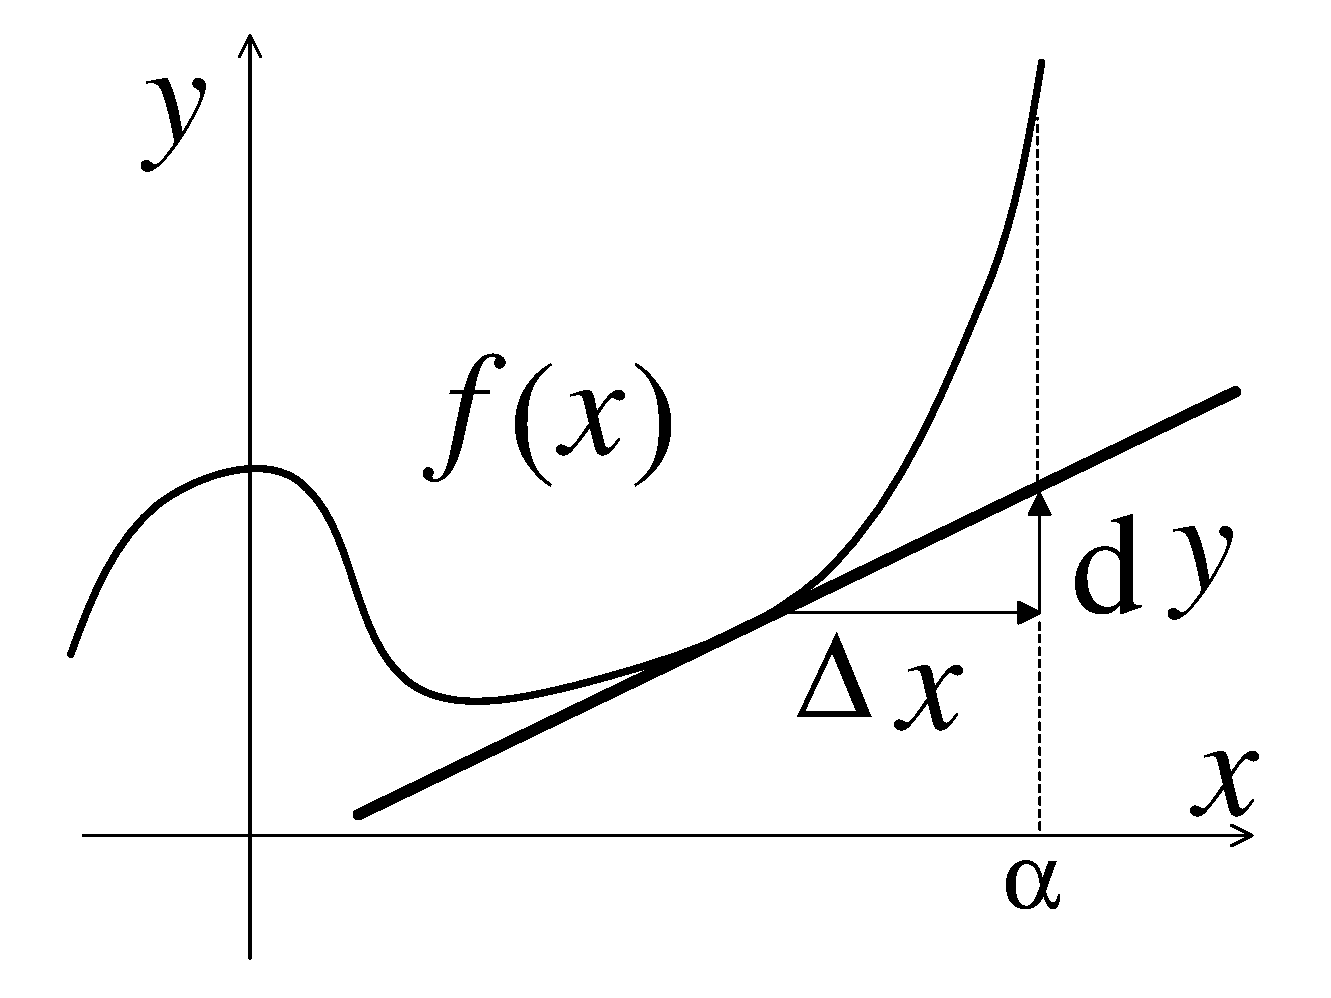
\includegraphics[keepaspectratio, width=6cm,height=2.4cm,clip]{bibunnno_Teigi00.pdf}
                        \caption{微分の定義}
                        \label{fig:bibunnno_Teigi00}
                    \end{center}
                \end{figure}

        %==================================================================
        %  SubSection
        %==================================================================
            \subsection{1次関数 $f(x)=ax+b$ の増加量}
                一次関数の増加量を,微分を使って表してみる.仰々しいかもしれないが,
                後でこの考え方を発展させるために,基礎的なところから考えていきたい.
                \begin{figure}[hbt]
                    \begin{center}
                        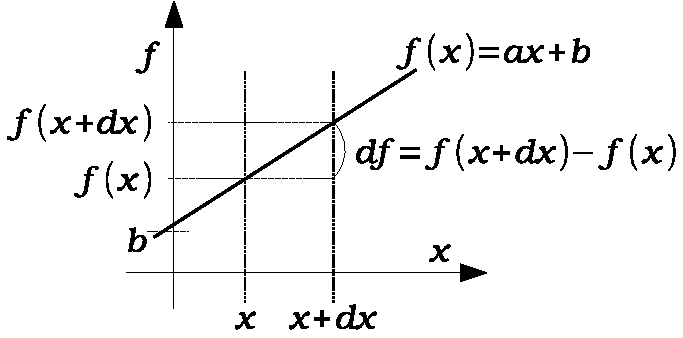
\includegraphics[keepaspectratio, width=6cm,height=2.85cm,clip]{ichi_hensu_kansu_zokaryo2.pdf}
                        \caption{1次関数数関数 $f(x)=ax+b$ の増加量}
                        \label{fig:ichi_hensu_kansu_zokaryo2}
                    \end{center}
                \end{figure}

                一次関数はグラフで表現すると直線であり,
                方程式は $f(x)=ax+b$ である.$a$ は傾きで,$b$ は $y$ 軸との交点である
                        \footnote{
                                $b$ は切片ともよばれる.
                        }.
                                点 $x$ のところでは,
                                        \begin{equation*}
                                                f(x) = ax + b.
                                        \end{equation*}
                                点 $x$ から微小距離 $\df x$ だけ離れたところでは($x+\df x$),
                                        \begin{equation*}
                                                f(x+\df x)=a(x+\df x)+b.
                                        \end{equation*}
                                よって, $x$ が $\df x$ だけ増えた時の $f(x)$ の増加量を $\df f$ として
                                        \footnote{
                                                より細かく表現すると,$\df f := \df f(x)$ である.
                                        },
                                        \begin{align*}
                                                \df f &= f(x+\df x) - f(x) \\
                                                      &= \{a(x+\df x)+b\} - \{ax + b\} \\
                                                      &= (ax + a\df x + b) - (ax + b) \\
                                                      &= a \df x.
                                        \end{align*}

                                一次関数の増加量は傾き $a$ と 微少変化 $\df x$ の積で表せることがわかった.

        %==================================================================
        %  SubSection
        %==================================================================
            \subsection{1変数関数 $f(x)$ の増加量}
                1変数関数 $f(x)$ において,$x$ の微小変化分 $\df x$ に対する $f(x)$ の
                増加量を計算したいことがある.これは,局所的に一次関数近似することで,
                一次関数の時と同じように考えることができる.
                \begin{figure}[hbt]
                    \begin{center}
                        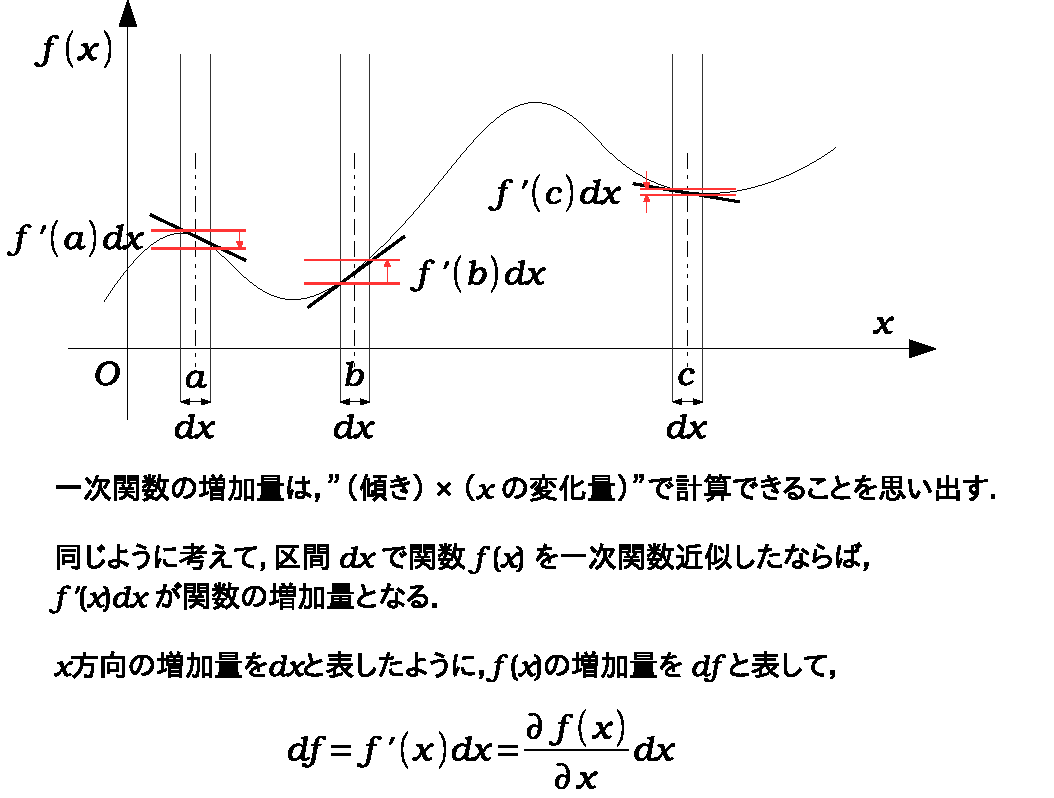
\includegraphics[keepaspectratio, width=7cm,height=6.7cm,clip]{ichi_hensu_kansu_zokaryo1.pdf}
                        \caption{1変数関数 $f(x)$ の増加量}
                        \label{fig:ichi_hensu_kansu_zokaryo1}
                    \end{center}
                \end{figure}

                                一次関数では,微小変化 $\df x$ に対する関数$f$の増加量は,
                                $\df f= a\df x$ と書けるのであった.
                                これを任意の一変数関数に拡張する場合,各$x$ で傾きが異なるが,$a=f'(x)$ と書けることを考慮すると,
                                        \begin{align}
                                                \df f = f'(x) \df x
                                        \end{align}
                                となる.これが1変数関数 $f(x)$ の増加量である.これはまさに,
                                前に説明した \textbf{微分} にほかならない.微分とは一変数関数の微小増加量のことをいうのである.

        %==================================================================
        %  SubSection
        %==================================================================
            \subsection{偏微分}
                次は2変数関数の微分だ.
                1変数関数のグラフは線であり,$x$方向の1方向のみを考えればよかった.
                これに対して,2変数の場合は面になるので,$x$方向と$y$方向の2方向を
                考える必要がある.

                $x$方向の微分をする場合は,$y$方向を固定して微分する.
                式で書くと,
                        \begin{equation*}
                                \frac{\rd f(x,\,y)}{\rd x}
                                := \lim_{\Delta x \to 0} \frac{f(x+\Delta x,\,y)-f(x,\,y)}{\Delta x}.
                        \end{equation*}
                $y$方向の微分をする場合は,$x$方向を固定して微分する.
                式で書くと,
                        \begin{equation*}
                                \frac{\rd f(x,\,y)}{\rd y}
                                := \lim_{\Delta y \to 0} \frac{f(x,\,y+\Delta y)-f(x,\,y)}{\Delta y}.
                        \end{equation*}
                このような微分を1変数の微分と区別するために
                        \footnote{
                                言い換えれば,多変数関数の微分であることを\textbf{強調}するために.
                        },
                \textbf{偏微分} という.

                偏微分の視点で,改めて,1変数の微分を見ると,$y=0$ 固定の微分であったと解釈できる.

        %==================================================================
        %  SubSection
        %==================================================================
            \subsection{全微分}
                偏微分の場合,微分するときに片方を固定してしまうので,$x$ と $y$ を"同時に"変化させた場合
                の関数の増加量がわからない.幸運なことに,$x$ と $y$ を"同時に"変化させた場合の増加量は,
                それぞれ独立であり,
                従って,「$x$ だけを変化させた場合の増加量」と「$y$ だけを変化させた場合の増加量」を
                たすだけで良い.
                \begin{figure}[hbt]
                    \begin{center}
                        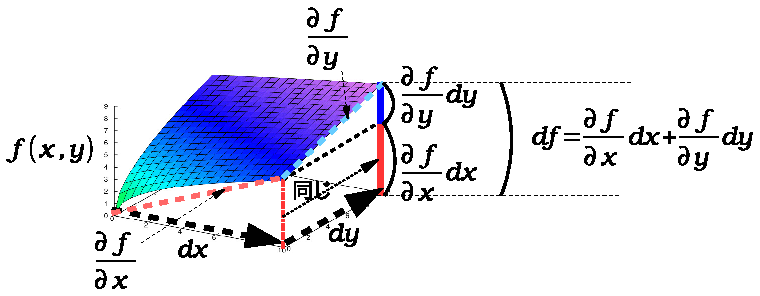
\includegraphics[keepaspectratio, width=7cm,height=4.096cm,clip]{gradient_sample_figure_0001.pdf}
                        \caption{全微分のイメージ}
                        \label{fig:gradient_sample_figure_0001}
                    \end{center}
                \end{figure}

                $x$ 方向だけ変化させた場合の増加量とは,$x$ 方向についての微分であり,
                \begin{equation*}
                     \frac{\rd f(x,\,y)}{\rd x} \df x
               \end{equation*}
                である.また,$y$ 方向だけ変化させた場合の増加量とは,$y$ 方向についての微分であり,
                \begin{equation*}
                    \frac{\rd f(x,\,y)}{\rd y} \df y
                \end{equation*}
                と書ける.よって,$\df f:=\df f(x,\,y)$ は
                \begin{align}
                        \df f = \frac{\rd f(x,\,y)}{\rd x} \df x + \frac{\rd f(x,\,y)}{\rd y} \df y
                \end{align}
                と計算することができる.
                このような2変数関数の微分のことを \textbf{全微分} という.

                もう一度まとめておく.1変数関数の微小増加量が微分であることを先に確認した.
                2変数関数の場合は方向が2つあるので,増加量を計算するには全方向の微分
                \footnote{
                    「全方向の微分」のことを「全独立変数の微分」と言い換えても良い.
                }
                を足し合わせる必要があった.全方向の増加分の和が全微分である.
                2変数以上の関数の微分は全て,全微分と言われる.

                



%   %==========================================================================
%   %  Section : 微分
%   %==========================================================================
        \section{よく使う公式}
%       %----------------------------------------------------------------------
%       %  Input
%       %    File Name : PhysNote_Math_Fomulas.tex
%       %    説明      : よく使われる公式の証明.
%       %----------------------------------------------------------------------
        %       %======================================================================
%       %  SubSection
%       %======================================================================
\subsection{和の微分}
    1変数関数 $K(x)$ があり,この $K(x)$ が2つの関数 $f(x)$,$g(x)$ の和に分解できるとする.
    つまり,以下が成り立っている場合を考える
        \footnote{
            ごく簡単な例で言えば,$K(x)=f(x)+g(x)=5x$,$f(x)=x$,$g(x)=4x$ の場合とか.
        }.
        \begin{equation*}
            K(x) = f(x) + g(x).
        \end{equation*}
    この時,
         \begin{align}
             K'(x) = f'(x) + g'(x)
         \end{align}
    が成り立つ.

    これは微分の定義に従って式変形をすることで,確認できる.少々面倒だが,やってみよう.
        \begin{align*}
            K'(x) &= \lim_{\Delta x \to 0} \frac{K(x+\Delta x)-K(x)}{\Delta x} \\
                  &= \lim_{\Delta x \to 0}
                     \frac{\left(f(x+\Delta x)+g(x+\Delta x)\right)-\left( f(x)+g(x)\right)}{\Delta x} \\
                  &= \lim_{\Delta x \to 0}
                     \frac{f(x+\Delta x)-f(x) + g(x+\Delta x)-g(x)}{\Delta x} \\
                  &= \lim_{\Delta x \to 0}
                     \left(
                         \frac{f(x+\Delta x)-f(x)}{\Delta x}+\frac{g(x+\Delta x)-g(x)}{\Delta x}
                     \right) \\
                  &= \lim_{\Delta x \to 0} \frac{f(x+\Delta x)-f(x)}{\Delta x}
                   + \lim_{\Delta x \to 0} \frac{g(x+\Delta x)-g(x)}{\Delta x} \\
                  &= f'(x) + g'(x).
        \end{align*}

    この式変形で,関数の極限の和の公式を利用している
        \footnote{
            $\displaystyle\lim_{x \to 0}f(x)$ と $\displaystyle\lim_{x \to 0}g(x)$ が共に収束する場合,
            \begin{equation*}
                \lim_{x \to 0}(f(x)+g(x)) = \lim_{x \to 0}f(x) + \lim_{x \to 0}g(x).
            \end{equation*}
        }.

\subsection{積の微分}
    1変数関数 $K(x)$ があり,この $K(x)$ が2つの関数 $f(x)$,$g(x)$ の積に分解できるとする.
    つまり,以下が成り立っている場合を考える
        \footnote{
            ごく簡単な例で言えば,$K(x)=f(x)g(x)=5x(x+1)$,$f(x)=5x$,$g(x)=x+1$ の場合とか.
        }.
        \begin{equation*}
            K(x) = f(x)g(x).
        \end{equation*}
     この時,
         \begin{align}
             K'(x) = f'(x)g(x) + f(x)g'(x)
         \end{align}
     が成り立つ.

    これは微分の定義に従って式変形をすることで,確認できる.少々面倒だが,やってみよう.
    特に,$-f(x)g(x+\Delta x) + f(x)g(x+\Delta x) = 0$ であることに注意.
        \begin{align*}
            &K'(x) \\
            &= \lim_{\Delta x \to 0}
               \frac{K(x+\Delta x)-K(x)}{\Delta x} \\
            &= \lim_{\Delta x \to 0}
               \frac{f(x+\Delta x)g(x+\Delta x)-f(x)g(x)}{\Delta x} \\
            &= \lim_{\Delta x \to 0}
               \frac{f(x+\Delta x)g(x+\Delta x)-f(x)g(x+\Delta x) + f(x)g(x+\Delta x)-f(x)g(x)}{\Delta x} \\
            &= \lim_{\Delta x \to 0}
               \frac{\left(f(x+\Delta x)-f(x)\right)g(x+\Delta x) + f(x)\left(g(x+\Delta x)-g(x)\right)}{\Delta x} \\
            &= \lim_{\Delta x \to 0} \frac{\left(f(x+\Delta x)-f(x)\right)g(x+\Delta x)}{\Delta x}
             + \lim_{\Delta x \to 0} f(x)\frac{g(x+\Delta x)-g(x)}{\Delta x} \\
            &= \lim_{\Delta x \to 0} \frac{f(x+\Delta x)-f(x)}{\Delta x} g(x+\Delta x)
             + f(x) \lim_{\Delta x \to 0} \frac{g(x+\Delta x)-g(x)}{\Delta x} \\
            &= f'(x)g(x) + f(x)g'(x).
        \end{align*}

    この式変形で,関数の極限の積の公式を利用している
        \footnote{
            $\displaystyle\lim_{x \to 0}f(x)$ と $\displaystyle\lim_{x \to 0}g(x)$ が共に収束する場合,
            \begin{equation*}
                \lim_{x \to 0}(f(x) \cdot g(x)) = \lim_{x \to 0}f(x) \cdot \lim_{x \to 0}g(x).
            \end{equation*}
        }.
    また,式変形について,以下を考慮した.
        \begin{align*}
            f(x) &= \lim_{\Delta x \to 0} f(x) \\
            g(x) &= \lim_{\Delta x \to 0} g(x+\Delta x)
        \end{align*}
    1つ目の式はそもそも $\Delta x$ が関数 $f(x)$ にないので,$\Delta x$ に関する極限を
    とったところで変化なし.2つ目の式は関数の極限の定義そのものである.

\subsection{商の微分}
    1変数関数 $K(x)$ があり,この $K(x)$ が2つの関数 $f(x)$,$g(x)$ の商に分解できるとする.
    つまり,以下が成り立っている場合を考える
        \footnote{
            ごく簡単な例で言えば,$K(x)=f(x)/g(x)=5x$,$f(x)=20{x}^{2}$,$g(x)=4x$ の場合とか.
        }.
        \begin{equation*}
            K(x) = \frac{f(x)}{g(x)}.
        \end{equation*}
    この時,
         \begin{align}
             K'(x) = \frac{f'(x)g(x) - f(x)g'(x)}{{\left(g(x)\right)}^{2}}
         \end{align}
    が成り立つ.

    これを示すには,
        \begin{equation*}
            K(x) = \frac{f(x)}{g(x)} = f(x)\frac{1}{g(x)}
        \end{equation*}
    とみなし,積の微分公式を用いる.実際に確認してみよう.
        \begin{equation*}
            K'(x) = f'(x)\frac{1}{g(x)} + f(x)\left(\frac{1}{g(x)}\right)'
        \end{equation*}
    ここで移行の式変形の都合上
        \footnote{
            不自然に思われるかもしれないが,覚えやすく使いやすい形にしたいがための式変形であり,
            重要な部分である.
        }
    ,上式の第1項の分母と分子に $g(x)$ をかけて,
        \begin{equation*}
            K'(x) = f'(x)g(x)\frac{1}{{g(x)}^{2}} + f(x)\left(\frac{1}{g(x)}\right)'
        \end{equation*}
    としておく.また,第2項のカッコ内の微分は,定義に従って計算する
        \footnote{
            2つの分数の恒等式を使うので,補足しておこう.
            \begin{equation*}
                \frac{1}{A} - \frac{1}{B}
                = \frac{B}{AB} - \frac{A}{AB}
                = \frac{B-A}{AB}
                = - \frac{A-B}{AB}.
            \end{equation*}
            \begin{equation*}
                \frac{\displaystyle\frac{A}{B}}{C}
                = \frac{\displaystyle\frac{A}{B}B}{BC}
                = \frac{A}{BC}.
            \end{equation*}
        }.
        \begin{align*}
            \left(\frac{1}{g(x)}\right)'
            &= \lim_{x \to 0}
               \frac{\displaystyle\frac{1}{g(x + \Delta x)} - \displaystyle\frac{1}{g(x)}}{\Delta x} \\
            &= \lim_{x \to 0}
               \frac{\displaystyle\frac{-g(x + \Delta x)+g(x)}{g(x + \Delta x)g(x)}}{\Delta x} \\
            &= \lim_{x \to 0}
               -\frac{g(x + \Delta x)-g(x)}{\Delta x}\frac{1}{{g(x + \Delta x)g(x)}} \\
            &= -g'(x) \frac{1}{{\left(g(x)\right)}^{2}} \\
            &= -\frac{g'(x)}{{\left(g(x)\right)}^{2}}
        \end{align*}
    なので,
        \begin{equation*}
            K'(x) = f'(x)g(x)\frac{1}{{g(x)}^{2}}-f(x)\frac{g'(x)}{{\left(g(x)\right)}^{2}}.
        \end{equation*}
    共通な分母でまとめると,
        \begin{equation*}
            K'(x) = \frac{f'(x)g(x)-f(x)g'(x)}{{\left(g(x)\right)}^{2}}.
        \end{equation*}

\subsection{合成関数の微分}
    関数 $f(g(x))$ というもの考える.$g(x)$ は独立変数 $x$ を持つ関数であり,$f$ は $g(x)$ で
    得られた値を引数に持つ関数である
        \footnote{
            例えば,${(x+1)}^{2}$ であれば,$g(x)=x+1$ として $f(g(x))={\left(g(x)\right)}^{2}$ と
            書き表せる.
        }.
    こういった入れ子になった関数を \textbf{合成関数} という.
    $f(g(x))$ は $(g \circ f)(x)$ と書かれることもある.
        \footnote{
            表記だけの問題だが,$f(g(x))$ という表現は,見難くなる傾向にある.この程度であれば,まだ
            わかるが,これが $f(g(h(i(j(x))))$ となった場合にはカッコが多くて,読み難くくなってしまう.
            だから,$f(g(x))=(g \circ f)(x)$ と書くこともある.これなら,関数が多くなろうとも問題ない.
            さっきの例で言うと,$(j \circ i \circ h \circ g \circ f) (x)$ である.
            関数の依存関係を左のカッコ内に書き,その独立変数を右のカッコの中に書く.関数の依存関係は
            一番深いものを最左に書き,順次右に追記していく.
        }.

    ここでは,この合成関数の微分公式を確認する.
    合成関数 $(g \circ f)(x)=f(g(x))$ は $u=g(x)$ と置いて $f(u)$ と見ることができる.
    $g(x)$ が $x$ の関数だから,結局のところ $(g \circ f)(x)$ も $x$ の関数となるので,
    $\df (g \circ f) /\df x$ を考えられる.$u=g(x)$ を展開し,さらに $f(u)$ を
    展開した後で,微分を計算しても良いが,もっと賢い方法がある.次のとおりだ.
        \begin{align}
            \frac{\df (g \circ f)}{\df x}
            = \frac{\df f}{\df u}\frac{\df u}{\df x}
            = \frac{\df f(u)}{\df u}\frac{\df g(x)}{\df x}.
        \end{align}

    これが正しいことは,微分の定義から計算することで確認できる.
        \begin{align*}
            &\frac{\df (g \circ f)}{\df x} \\
            &= \lim_{\Delta x \to 0}
               \frac{(g \circ f)(x+\Delta x)-(g \circ f)(x)}{\Delta x} \\
            &= \lim_{\Delta x \to 0}
               \frac{(g \circ f)(x+\Delta x)-(g \circ f)(x)}{g(x + \Delta x) - g(x)}
               \frac{g(x + \Delta x) - g(x)}{\Delta x} \\
            &= \lim_{\Delta x \to 0}
               \frac{(g \circ f)(x+\Delta x)-(g \circ f)(x)}{\Delta g}
               \frac{g(x + \Delta x) - g(x)}{\Delta x} \\
            &= \lim_{\Delta x \to 0}
               \frac{(g \circ f)(x+\Delta x)-(g \circ f)(x)}{g(x + \Delta x) - g(x)}
               \cdot
               \lim_{\Delta x \to 0}
               \frac{g(x + \Delta x) - g(x)}{\Delta x}
        \end{align*}

    ここで,式の見やすさのため,$\Delta g = g(x + \Delta x) - g(x)$ と置く.
    また,$g(x)=\displaystyle \lim_{\Delta x \to 0} g(x+\Delta x)$ の関係から,
        \begin{align*}
            &\lim_{\Delta x \to 0} \left( g(x+\Delta x) \right) - g(x) \\
            &= \lim_{\Delta x \to 0} \left( g(x+\Delta x) - g(x) \right) \\
            &= \lim_{\Delta x \to 0} \Delta g \\
            &= 0
        \end{align*} \\
    が成り立つので,$\Delta x \to 0$ を $\Delta g \to 0$ に置き換えられることを使う.
        \begin{flalign*}
            &\frac{\df (g \circ f)}{\df x} \\
                                &= \lim_{\Delta g \to 0}
                                   \frac{(g \circ f)(x+\Delta x)-(g \circ f)(x)}{\Delta g}
                                   \cdot
                                   \lim_{\Delta x \to 0}
                                   \frac{g(x + \Delta x) - g(x)}{\Delta x}
        \end{flalign*}

    最後に,$\Delta (g \circ f) = (g \circ f)(x+\Delta x)-(g \circ f)(x) $,
    $\Delta u = \Delta g$ であることに注意すれば,
        \begin{flalign*}
            \frac{\df (g \circ f)}{\df x}
                &= \lim_{\Delta g \to 0} \frac{\Delta (g \circ f)}{\Delta g}
                   \cdot
                   \lim_{\Delta x \to 0} \frac{g(x + \Delta x) - g(x)}{\Delta x} \\
                &= \lim_{\Delta u \to 0} \frac{\Delta (g \circ f)}{\Delta u}
                   \cdot
                   \lim_{\Delta x \to 0} \frac{\Delta g}{\Delta x} \\
                &= \lim_{\Delta u \to 0} \frac{\Delta (g \circ f)}{\Delta u}
                   \cdot
                   \lim_{\Delta x \to 0} \frac{\Delta u}{\Delta x} \\
                &= \frac{\df (g \circ f)}{\df u} \frac{\df u}{\df x}
        \end{flalign*}
    を得る.大抵の場合は,$f:=(g \circ f)=f(g(x))$ と略記されるので,これに従うと,
        \begin{flalign*}
            \frac{\df f}{\df x} &= \frac{\df f}{\df u} \frac{\df u}{\df x}
        \end{flalign*}
    となって,いつもの合成関数の微分公式が見えてくる.

\subsection{部分積分}





\chapter{微分方程式}
%   %-----------------------------------------------------------------------------------------------
%   %  Input
%   %    File Name : PhysNote_Math_DifrEq.tex
%   %    説明      : 「微分積分学」について.考え方と使い方.
%   %-----------------------------------------------------------------------------------------------
        %===================================================================================================
%  Chapter : 微分方程式
%  説明    : 微分方程式の考え方と計算方法を確認する.
%===================================================================================================
%   %==========================================================================
%   %  Section : 微分方程式とは
%   %==========================================================================
        \section{微分方程式とは}
%       %----------------------------------------------------------------------
%       %  Input
%       %    File Name : PhysNote_Math_DifrAndIntg_inf.tex
%       %    説明      : 微分方程式の定義など
%       %----------------------------------------------------------------------
        %   %==========================================================================
%   %  Section : 微分方程式とは
%   %==========================================================================
        %==================================================================
        %  SubSection
        %==================================================================
            \subsection{微分方程式の概要}
                


\chapter{ベクトル}
%   %-----------------------------------------------------------------------------------------------
%   %  Input
%   %    File Name : PhysNote_Math_Vector.tex
%   %    説明      : 「ベクトル」について.考え方と使い方.
%   %-----------------------------------------------------------------------------------------------
        %===================================================================================================
%  Chapter : ベクトル
%  説明    : ベクトルの考え方と計算方法を確認する.
%===================================================================================================
%   %==========================================================================
%   %  Section : ベクトルの定義
%   %==========================================================================
        \section{ベクトルの定義}
%       %----------------------------------------------------------------------
%       %  Input
%       %    File Name : PhysNote_Math_Vector_def.tex
%       %    説明      : ベクトルを定義する
%       %----------------------------------------------------------------------
        %   %==========================================================================
%   %  Section : ベクトルの定義
%   %==========================================================================
        %==================================================================
        %  SubSection
        %==================================================================
            \subsection{図形的(幾何学的)なベクトル}
                物理を考える上で,\textbf{矢印} はとても有用である.
                力の方向と大きさを直感的に表現するのに,矢印は欠かせない.
                この矢印は,数学的に扱うことができて,数学の世界では,
                矢印のことを \textbf{ベクトル} とよんでいる.

                矢印のトンガリがない方を,矢印の \textbf{始点} といい,
                トンガっている方を,矢印の \textbf{終点} という.
                これにより,方向は矢印の向きで表現できるし,その大きさは
                長さに比例するように描くと約束すれば,大きさも表現できる.
                イメージは,図\ref{fig:yajirusi_vector}に描いたようになる
                    \footnote{
                        当たり前すぎて,描くまでもなかったかな.
                    }.
                        \begin{figure}[hbt]
                            \begin{center}
                                \includegraphicsdefault{yajirusi_vector.pdf}
                                \caption{ベクトル:図形,矢印}
                                \label{fig:yajirusi_vector}
                            \end{center}
                        \end{figure}

                これを文字で表すと,始点を $\mathrm{O}$ とし,また,終点を $\mathrm{P}$ とする
                線分 $\overline{\mathrm{OP}}$ に向きをつけたと考えて,
                    \begin{equation*}
                        \overrightarrow{\mathrm{OP}}
                    \end{equation*}
                と書ける.

            \begin{memo}{ベクトルの位置は不問である}
                同じ大きさで,同じ向きをもつベクトルがいくつか存在する
                場合を考える.これらのベクトルの位置が異なる場合,
                異なるベクトルと考えるべきなのだろうか.
                        \begin{figure}[hbt]
                            \begin{center}
                                \includegraphicsdefault{OnajiVector.pdf}
                                \caption{ベクトル:図形,矢印}
                                \label{fig:OnajiVector}
                            \end{center}
                        \end{figure}

                結論から書くと,これらのベクトルは,同一とみなされる.
                つまり,ベクトルの存在する場所は,そのベクトルの性質
                には何ら関係がないということだ.そもそも,ベクトルと
                は大きさと向きのみをもつ概念であるから,当然,ベクトルが
                同一であるということは,大きさと向きが同じであるということ
                である.ベクトルが存在する場所は,定義には含まれておらず,
                不問とされるのである.

                ベクトルという概念は,力学を数式化するために整備されたものである.
                ベクトルを用いることで,物体にかかる力を数式で表現できるように
                なるのだ.例えば,自分が誰かから引っ張られる場合を想像してみよう.
                同じ大きさの力で,同じ向きに引っ張られるのであれば,引っ張られる
                場所は関係ない.引っ張られる場所が,公園だろうが,公民館だろうが,
                あるいはトイレだろうが,引っ張られるときの感覚は同一のはずである.
                つまり,力そのものは,その発生場所には関係がないのである.ベクトル
                という概念は力学の記述に適するようにつくられたので,力と同様に,
                その存在する場所には依存しないのである.というか,依存しないと定義
                付けるのである
                    \footnote{
                        ベクトルの定義では,場所に依存しないという直接的な記述はないが,
                        定理として成り立つ性質として,このことが保証される.場所に
                        依存しないように定義付けを行っているんだから,当たり前だ.
                    }.
                いつどんな場所でも,
                同じ物体に同じ力をかければ,その位置の変化の仕方もまた同じなのである.
                いや,結果が同じになるように,ベクトルという概念を定義してしまうのだ.
            \end{memo}

        %==================================================================
        %  SubSection
        %==================================================================
            \subsection{代数的なベクトル}
            \begin{mycomment}
                ベクトルを数式で扱えるように,是非とも,
                文字を使ってベクトルを表現したい.
                ベクトルは代数的に表現可能なのだが
                    \footnote{
                        「代数的に表現可能」とは,文字の列として表現
                        することが可能であるということである.
                    },
                2つの書き方がある.書き方の違いにより,次のように
                言葉を割当て,区別する.すなわち,
                    \begin{itemize}
                        \item 横ベクトル
                        \item 縦ベクトル
                    \end{itemize}
                なぜこう言われるかは,後の記述で分かることなので,
                今は気にせず,話を進めよう.
                横ベクトル$\cdot$縦ベクトル共に,どちらも同じように頻繁に使われる.
                どっちも大切である.どちらか一方を採用したら,他方を捨て去るということ
                はない.
            \end{mycomment}

            %==============================================================
            %  SubsubSection
            %==============================================================
                \subsubsection{横ベクトル}
                ベクトルを代数的に表現する方法は2通りあると,先に記述した.
                ここではそのうちの,\textbf{横ベクトル} について,説明する.

                ベクトルをどのように代数的に表現するのか.実は,
                その考え方は簡単で,そのベクトルの始点に原点 $O$ を合わせた
                座標を張ればよい.図\ref{fig:yajirusi_vector_daisu}では
                直交直線座標を描いた.これより,終点の座標を記述する
                ことで,ベクトルを表現できるのである.
                        \begin{figure}[hbt]
                            \begin{center}
                                \includegraphicsdefault{yajirusi_vector_daisu.pdf}
                                \caption{ベクトル:図形,矢印}
                                \label{fig:yajirusi_vector_daisu}
                            \end{center}
                        \end{figure}

                代数的なベクトルは,以下のように記述される.
                    \begin{align}
                        \br = \left[\,x\,,y\,\right].
                    \end{align}
                上の表現では,2次元の平面に存在するベクトルが記述されている.より高次元の
                ベクトル $\bx$ を考える場合,その次元数を $n$ として,
                    \begin{align}
                        \bx = \left[\,x_{1}\,,\,\,x_{2}\,,\,\,\cdots\,,\,\,x_{n}\,\right].
                    \end{align}
                ここで,座標を表すこ記号を,$x$ に統一して添字により区別すよう,
                表現方法を変えた.

                このように,成分を横書きしたベクトル表記を,\textbf{横ベクトル} という.

                ベクトルを表現するのに,太字を用いているのは,単なる実数と
                区別するためである.

            %==============================================================
            %  SubsubSection
            %==============================================================
                \subsubsection{縦ベクトル}
                    横ベクトルが成分を横書きしたベクトル表現だとしたら,
                    \textbf{縦ベクトル} とは成分を縦書きしたベクトル表現である.
                    なんとも安易な考え方だ.縦ベクトルは以下のように記述される.
                    \begin{align}
                        \bx
                        =
                        \left[
                            \begin{array}{c}
                                x_{1} \\
                                x_{2} \\
                                \vdots \\
                                x_{n} \\
                            \end{array}
                        \right].
                    \end{align}

        %==================================================================
        %  SubSection
        %==================================================================
            \subsection{ベクトルの大きさ}
                ベクトルの大きさは,三平方の定理により定義できる
                    \footnote{
                        三平方の定理について一言コメントしておこう.
                        これは数学的には三角関数の余弦定理の特殊な場合である.
                        しかし,ここでは,三平方の定理を距離を定めるひとつの要請
                        として扱うことにする.
                    }.

                まず,2次元ベクトル $\br=\left[\,x\,,y\, \right]$ の場合,このベクトルの
                大きさは三平方の定理によって定められ,
                    \begin{align}
                        |\br| = \sqrt{x^{2} + y^{2}}
                    \end{align}
                である.
                        \begin{figure}[hbt]
                            \begin{center}
                                \includegraphicsdefault{SanHeihouNoTeiri_2D_01.pdf}
                                \caption{三平方の定理(2次元)}
                                \label{fig:SanHeihouNoTeiri_2D_01}
                            \end{center}
                        \end{figure}

                2次元のベクトルの大きさを,3次元ベクトルに拡張しよう.
                図\ref{fig:SanHeihouNoTeiri_3D_01}の色を塗った部分の
                直角三角形に着目する.このとき,2次元の三平方の定理から,
                    \begin{equation*}
                        |\br| = \sqrt{\left(\sqrt{x^{2} + y^{2}}\right)^{2} + z^{2}}
                    \end{equation*}
                が成立している.つまり,
                    \begin{align}
                        |\br| = \sqrt{{x}^{2} + {y}^{2} + {z}^{2}}
                    \end{align}
                という関係があるということだ.もはや変数は4つであり,
                "三平方"という語彙と食い違ってしまったが,とりあえず,
                ここでは,3次元の三平方の定理と表現しておこう.
                        \begin{figure}[hbt]
                            \begin{center}
                                \includegraphicslarge{SanHeihouNoTeiri_3D_01.pdf}
                                \caption{三平方の定理(3次元)}
                                \label{fig:SanHeihouNoTeiri_3D_01}
                            \end{center}
                        \end{figure}

        %==================================================================
        %  SubSection
        %==================================================================
            \subsection{ベクトルの次元}
            私たちは,3次元の世界に住んでいるから,当然,縦$\cdot$横$\cdot$高さ
            の3方向しか把握できない.4つ以上の次元で成り立つ世界を見ることは
            不可能である.しかし,数学的には,4つ以上の方向を考えても,理論的
            に矛盾することはない.つまり,数学的には,より多くの方向をもつベクトルを
            扱えるのである
                \footnote{
                    ただし,4つ以上の方向を肌で感じたり,見たりできない以上,
                    図示することは不可能であるから,4次元以上の世界は完全に
                    文字(数式)だけの記述のみになってしまう.
                }.
            そこで,4つ以上の方向をもつベクトルについて,考える.

            まず,今まで日常生活的に使用してきた,\textbf{次元} という語彙を,
            数学用語として改めてその意味を明確にしておきたい.次元とは,ベクトルの
            成分の個数と定める.ただし,物理学では単位のことを次元と表現するが
                \footnote{
                    物理学では「次元解析」という言葉が使われる.これは,物理学的な単位
                    同士の関係を調べることであり,特に,数式の右辺と左辺の単位に矛盾が
                    ないかを確認することで利用される.しかし,ここで考えている次元とは,
                    意味が異なる(完全に異なるわけではないが)ものとして,考えてもらいたい.
                    少なくとも,いま考える次元とは,空間の方向の数であり,ベクトルの
                    成分の個数のことである.
                },
            それとは別物である.

            あるベクトル $\br$ があり,その成分が $n$ 個であるとしよう.つまり,
                \begin{equation*}
                    \br = \left[r_{1},\,r_{2},\,r_{3},\,\cdots,\,r_{n}\right]
                \end{equation*}
            と成分表示されるとする.この時,$\br$ のことを \textbf{$n$ 次元ベクトル} と
            いう.

                \begin{memo}{$n$ 次元の三平方の定理}
                    2次元と3次元の両方の三平方の定理から推察して,
                    より高次元である $n$ 次元に定理を拡張できる.
                    もちろん,$n$ は任意の自然数である.
                    この拡張に伴って,この定理に改めて名前をつける
                    ことにしよう
                        \footnote{
                            これから定義しようとするのは,$n$ 次元での定理
                            であり,それには $n+1$ 個の数が絡んでくるから,
                            「三平方の定理」では定理の内容と一致しなくなってしまう
                            のだ.
                        }.
                    \textbf{距離の公理} と名付ける.

                    $n$ 次元への拡張は以下のようにして行われる.
                    \begin{align}
                        r := |\br|
                           = {q_{1}}^{2} + {q_{2}}^{2} + \cdots + {q_{n}}^{2}
                           = \sqrt{\sum_{i=1}^{n} {q_{i}}^{2}}.
                    \end{align}
                    ここに,$q_{i}$ はそれぞれ座標を表す.
                \end{memo}

        %==================================================================
        %  SubSection
        %==================================================================
            \subsection{ベクトル空間の定義}
                ベクトルをより一般的に定義しておきたい.そこで,はじめに,
                ベクトルの集合を定義する.ベクトルの持つ性質を列挙して,
                それを満たすものを,\textbf{ベクトル空間} とよぶ.そして,
                ベクトルをベクトル空間の要素として定義することで,ベクトル
                を,数学的に曖昧さのない概念として,扱うことが可能になる.
                    \\
                    \begin{itembox}[l]{\textbf{ベクトル空間}}
                        \begin{dfn}
                            ある集合 $\bU$ が次の条件全てを満たすとき,$\bU$ を \textbf{ベクトル空間} という.

                                集合 $\bU$ の任意の要素 $\ba$,$\bb$,$\bc$ に対して,
                                \begin{description}
                                    \item[\;\;\;1]\;\;\; $(\ba + \bb) + \bc = \ba + (\bb + \bc) $
                                    \item[\;\;\;2]\;\;\; $\ba + \bb = \bb + \ba$
                                    \item[\;\;\;3]\;\;\; $\bo + \ba = \bo$ を満たす $\bo$ がただ一つ存在する.
                                    \item[\;\;\;4]\;\;\; $\ba + \ba' = \bo$ を満たす $\ba'$ がただ一つ存在する.
                                \end{description}
                                が成立する.

                                さらに,任意の実数 $m$,$n$ に対して,
                                \begin{description}
                                    \item[\;\;\;5]\;\;\; $(m + n) \ba = m\ba + n\ba$
                                    \item[\;\;\;6]\;\;\; $m( \ba + \bb )$
                                    \item[\;\;\;7]\;\;\; $(mn)\ba = m(n\ba)$
                                    \item[\;\;\;8]\;\;\; $1\ba = \ba$
                                \end{description}
                                が成立する.

                            特に,$\bo = (\,0,\,0,\, \cdots,\,0\,)$ であり,\textbf{ゼロベクトル} という.
                        \end{dfn}
                    \end{itembox}
                    \\

        %==================================================================
        %  SubSection
        %==================================================================
            \subsection{ベクトルの定義}
                ベクトルを定義しよう.
                \\
                \begin{itembox}[l]{\textbf{ベクトル}}
                    \begin{dfn}
                        ベクトル空間 $\bU$ の要素のことを \textbf{ベクトル} という.
                    \end{dfn}
                \end{itembox}
                \\


%   %==========================================================================
%   %  Section : ベクトルの性質
%   %==========================================================================
        \section{ベクトルの性質}
%       %----------------------------------------------------------------------
%       %  Input
%       %    File Name : PhysNote_Math_Vector_AddSubMul.tex
%       %    説明      : ベクトルの加法,スカラー倍などを説明する
%       %----------------------------------------------------------------------
                %======================================================================
        %  SubSection
        %======================================================================
        \subsection{ベクトルの転置}
            横ベクトルと縦ベクトルの関係を,ここに書いておこう.
            議論の最初に,横ベクトルで表現したベクトルを,縦ベクトル
            として表現したい場合が起こる
                \footnote{
                    特に,ベクトルの内積を行列的に記述したい場合に,
                    このような要求をしたくなる.
                }

            そんな時,活躍するのが,ベクトルの \textbf{転置} という
            考え方である.

            $n$ 次元ベクトル $\bx$ を最初に導入するとき,
            横ベクトルとして定義したとする.そして,議論の途中,
            $\bx$ を縦ベクトルとして記述したくなったとしよう.
            すなわち,以下のような書き換えたいのである.
            \begin{align*}
                \left[\,x_{1}\,,\,\,x_{2}\,,\,\,\cdots\,,\,\,x_{n}\,\right]
                \quad \rightarrow \quad
                \left[
                    \begin{array}{c}
                        x_{1} \\
                        x_{2} \\
                        \vdots \\
                        x_{n} \\
                    \end{array}
                \right]
            \end{align*}
            要するに,横ベクトルの成分表示で,その成分を左から順に書いていたベクトルを,
            縦に上から順に成分を記述する方式に変更したいのだ.
            この操作を,ベクトルの \textbf{転置} という.

            この場合,以下のように記述する.
            \begin{align}
                {}^{t}\left[\,x_{1}\,,\,\,x_{2}\,,\,\,\cdots\,,\,\,x_{n}\,\right]
                =
                \left[
                    \begin{array}{c}
                        x_{1} \\
                        x_{2} \\
                        \vdots \\
                        x_{n} \\
                    \end{array}
                \right].
            \end{align}

            左辺の左上の添字 ${}^{t}$ で,ベクトルの転置を表現する.

            最初に定義されたベクトルが縦ベクトルであっても,
            ベクトルの転置を行うことで,横ベクトルにできる.
            つまり,次のようにも記述して良い.
            \begin{align}
                    \begin{array}{c}
                        {}^{t}
                        \\
                        \\
                        \\
                        \\
                    \end{array}
                \left[
                    \begin{array}{c}
                        x_{1} \\
                        x_{2} \\
                        \vdots \\
                        x_{n} \\
                    \end{array}
                \right]
                =
                \left[\,x_{1}\,,\,\,x_{2}\,,\,\,\cdots\,,\,\,x_{n}\,\right]
            \end{align}

            以上から,ベクトルの転置について,次が成立している.
            \begin{align}
               {}^{t} ({}^{t}\bx) = \bx.
            \end{align}

            ベクトル $\bx$ に2回転置をすれば,元のベクトルに戻るのである.
            以下のような感じで,巡回が起こる.
            \begin{align*}
                \mbox{縦ベクトル}
                    \xrightarrow[\mbox{\small{転置}}]{} \mbox{横ベクトル}
                    \xrightarrow[\mbox{\small{転置}}]{} \mbox{縦ベクトル} \\
                \mbox{横ベクトル}
                    \xrightarrow[\mbox{\small{転置}}]{} \mbox{縦ベクトル}
                    \xrightarrow[\mbox{\small{転置}}]{} \mbox{横ベクトル}
            \end{align*}

            もちろん,横ベクトルで表現しようとも,縦ベクトルで表現
            しようとも,同一のベクトルであれば,それが示すベクトルは同一
            である.同じベクトルを表現する方法が2種類あるということであり,
            ベクトルが2つになるわけではない.$\bx$ も ${}^{t}\bx$ も同じ
            ベクトルを表現するものであり,違うのは表現の方法なのだ.

        %==================================================================
        %  SubSection
        %==================================================================
            \subsection{ベクトルの四則演算}
            \begin{mycomment}
                ここでは,ベクトルに対して四則演算を定義する.
            \end{mycomment}

            %==============================================================
            %  SubSection
            %==============================================================
            \subsubsection{ベクトルの加法}
            3次元の2つのベクトルを,任意にもってきて,それらを
            \begin{equation*}
                \bx =
                \left[
                    \begin{array}{c}
                        x_{1} \\
                        x_{2} \\
                        x_{3} \\
                   \end{array}
                \right]\quad , \qquad
                \by =
                \left[
                    \begin{array}{c}
                        y_{1} \\
                        y_{2} \\
                        y_{3} \\
                   \end{array}
                \right]
            \end{equation*}
            と書くことにしよう.
            これら2つのベクトル $\bx$,$\by$ の和 $\bx + \by$ は,成分表示で
            以下のように示される.
                    \begin{align}
                        \bx + \by
                        =
                        \left[
                            \begin{array}{c}
                                x_{1} \\
                                x_{2} \\
                                x_{3} \\
                            \end{array}
                        \right]
                        +
                        \left[
                            \begin{array}{c}
                                y_{1} \\
                                y_{2} \\
                                y_{3} \\
                            \end{array}
                        \right]
                        =
                        \left[
                            \begin{array}{c}
                                x_{1} + y_{1} \\
                                x_{2} + y_{2} \\
                                x_{3} + y_{3} \\
                            \end{array}
                        \right].
                    \end{align}

                    つまり,成分同士を足し合わせるということである.

                    $n$ 次元ベクトルに対して,拡張しておこう.
                    任意の 2つの $n$ 次元ベクトル
                    \begin{equation*}
                        \bx =
                        \left[
                            \begin{array}{c}
                                x_{1} \\
                                x_{2} \\
                                \vdots \\
                                x_{n} \\
                           \end{array}
                        \right]\quad , \qquad
                        \by =
                        \left[
                            \begin{array}{c}
                                y_{1} \\
                                y_{2} \\
                                \vdots \\
                                y_{n} \\
                           \end{array}
                        \right]
                    \end{equation*}
                    に対して,これらの和は,成分で書くと次のようになる.
                    \begin{align}
                        \bx + \by
                        =
                        \left[
                            \begin{array}{c}
                                x_{1} \\
                                x_{2} \\
                                \vdots \\
                                x_{n} \\
                            \end{array}
                        \right]
                        +
                        \left[
                            \begin{array}{c}
                                y_{1} \\
                                y_{2} \\
                                \vdots \\
                                y_{n} \\
                            \end{array}
                        \right]
                        =
                        \left[
                            \begin{array}{c}
                                x_{1} + y_{1} \\
                                x_{2} + y_{2} \\
                                \vdots \\
                                x_{n} + y_{n} \\
                            \end{array}
                        \right].
                    \end{align}

                    また,次元の違うベクトル同士の和は定義されない.
                    つまり,次元が違うと,加法を行うことはできない.

            %==============================================================
            %  SubSection
            %==============================================================
            \subsubsection{実数とベクトルの積}
                ここでは,ひとつの任意の実数と,ひとつの任意のベクトルの
                積を定義する.ベクトル同士の掛け算も定義されるが
                    \footnote{
                        ベクトルの内積$\cdot$外積を参照.
                    },
                ここでは,実数とベクトルの掛け算のみについて考える.

                任意の実数 $a$ と任意の $n$ 次元ベクトル $\bx$ をもってきて,
                積を作る.その積を,
                    \begin{equation*}
                        a\bx
                        =
                        a\left[
                        \begin{array}{c}
                            x_{1}  \\
                            x_{2}  \\
                            \vdots \\
                            x_{n}  \\
                        \end{array}
                    \right]
                    \end{equation*}
                と書くことにする.成分で書くと,次のようになる
                    \footnote{
                        というか,こうなるように,実数とベクトルの積を
                        定義する.
                    }.
                \begin{align}
                    a\bx
                    =
                    a\left[
                        \begin{array}{c}
                            x_{1}  \\
                            x_{2}  \\
                            \vdots \\
                            x_{n}  \\
                        \end{array}
                    \right]
                    =
                    \left[
                        \begin{array}{c}
                            ax_{1}  \\
                            ax_{2}  \\
                            \vdots \\
                            ax_{n}  \\
                        \end{array}
                    \right].
                \end{align}

                これは $n$ 次元ベクトルに対して成り立つものである.
                つまり,実数とベクトルの積は,ベクトルの各成分を
                実数 $a$ 倍するということである.

            %==============================================================
            %  SubSection
            %==============================================================
            \subsubsection{ベクトルの減法}
                実数の世界では,事実上,減法が存在するが,しかしこれは公理的
                視点からは加法の一部である.つまり,2つの実数 $x$,$y$ があった
                時,減法 $x-y$ は 加法 $x+(-1 \cdot y)$ で定義されるのである.
                負の記号 $-1$ は公理により,その存在が示されているからである.
                減法を新たに定義するよりも,$-1$ の存在を主張するほうが,理論が
                単純になるり,思考経済
                    \footnote{
                        \textbf{思考経済}\quad
                        同じことを説明するのに,2つ以上の手段があるとしよう.
                        思考経済とは,この2つの説明のうちどちらを採用するかという
                        基準である.「簡潔に説明できる方を採用せよ」というものだ.
                        もちろん,最も簡潔に説明するほうがいいに決まっている(直感だけど)
                        うだうだ説明するりも,スパッと説明したほうが
                        かっこいいし,覚えることも少なくすむし,何しろ短時間で
                        説明できるのだから.しかし,世の中にはどちらも同じだけ
                        簡潔に説明できることが多くある.その場合には,時と場合に
                        よって使い分ける必要が出てくることだろう.
                    }
                に合致する.

                ベクトルに関する減法も,実数と同様に,加法の一部として,説明される
                べきものである.負の向きをもつベクトルとは,当然,正の向きに対して
                逆向きのベクトルである.負の向きのベクトルは,ベクトルに $-1$ を掛
                けることで,得られる.つまり,任意の $n$ 次元ベクトル $\by$ に対して,
                これと同じ大きさで,逆向きのベクトルは,
                \begin{equation*}
                    -1 \cdot \by = -\by
                \end{equation*}
                と書かれる.実数の場合と同じように,$-1$ 倍のときは,$1$を省略して
                書くことにする.

                これを用いて,ベクトルの減法を定めよう.
                任意の 2つの $n$ 次元ベクトル $\bx$,$\by$ に対して,差
                $\bx - \by$ とは次のように,成分表示される.
                \begin{align}
                    \bx - \by &= \bx + (- \by) \notag \\
                    &=
                    \left[
                        \begin{array}{c}
                            x_{1}  \\
                            x_{2}  \\
                            \vdots \\
                            x_{n}  \\
                        \end{array}
                    \right]
                    +
                    (-1)\left[
                        \begin{array}{c}
                            y_{1}  \\
                            y_{2}  \\
                            \vdots \\
                            y_{n}  \\
                        \end{array}
                    \right] \notag \\
                    &=
                    \left[
                        \begin{array}{c}
                            x_{1}  \\
                            x_{2}  \\
                            \vdots \\
                            x_{n}  \\
                        \end{array}
                    \right]
                    +
                    \left[
                        \begin{array}{c}
                            -y_{1}  \\
                            -y_{2}  \\
                            \vdots \\
                            -y_{n}  \\
                        \end{array}
                    \right] \notag \\
                    &=
                    \left[
                        \begin{array}{c}
                            x_{1}  +(-y_{1}) \\
                            x_{2}  +(-y_{2}) \\
                            \vdots \\
                            x_{n}  +(-y_{n}) \\
                        \end{array}
                    \right] \notag \\
                    \therefore \quad
                    \bx - \by
                    &=
                    \left[
                        \begin{array}{c}
                            x_{1}  -y_{1} \\
                            x_{2}  -y_{2} \\
                            \vdots \\
                            x_{n}  -y_{n} \\
                        \end{array}
                    \right]
                \end{align}



%       %----------------------------------------------------------------------
%       %  Input
%       %    File Name : PhysNote_Math_Vector_NaiSekiGaiSeki.tex
%       %    説明      : ベクトルのもつ性質(内積など)を考える
%       %----------------------------------------------------------------------
        %   %==========================================================================
%   %  Section : ベクトルの性質
%   %==========================================================================
        %==================================================================
        %  SubSection
        %==================================================================
            \subsection{ベクトルの内積(図形的)}\label{subsec:VecNaisekiFig}
                ベクトルの内積について,簡単に説明をしておこう.

                2つの任意のベクトルを用意し,$\ba$,$\bb$ とする.ベクトルの \textbf{内積} は
                この2つのベクトルより定義される.
                内積の表し方は,$(\ba\,,\;\bb)$ または $\ba\cdot\bb$ などの複数の表現がある.
                このノートでは,$\ba\cdot\bb$ を内積の記号として使うことにする.
                ベクトルの内積を,次のように,平面図形的に定義する.
                    \\
                    \begin{itembox}[l]{\textbf{ベクトルの内積(図形的)}}
                        \begin{dfn}
                            任意の2つのベクトル $\ba$ と $\bb$ の間に,演算 $\cdot$ を
                            以下のように定義する.
                            \begin{align}
                                 \ba\cdot\bb := | \ba |  | \bb | \cos\theta
                            \end{align}
                            この演算を,ベクトル $\ba$ と $\bb$ の \textbf{内積} という.
                        \end{dfn}
                    \end{itembox}
                    \\

                この式のイメージは,「$\ba$ の $\bb$ 方向の成分の大きさ」と,$\bb$ の積の大きさである.
                    \begin{equation*}
                        \ba\cdot\bb = ( | \ba | \cos\theta ) | \bb |
                    \end{equation*}
                と書いたらイメージしやすい.$| \ba | \cos\theta$ の $|\bb|$ 倍ということである.

                    \begin{figure}[hbt]
                        \begin{center}
                            \includegraphicsdefault{bekutoru_no_naiseki.pdf}
                            \caption{内積}
                            \label{fig:bekutoru_no_naiseki}
                        \end{center}
                    \end{figure}

                例えば,$\theta = 60{}^{\circ}$,$| \ba | = 3$,$| \bb | = 5$ のとき,
                    \begin{align*}
                        \ba\cdot\bb     &= | \ba |  | \bb | \cos\theta = 3 \times 5 \times \cos(60{}^{\circ}) \\
                                            &= 3 \times 5 \times \frac{1}{2} \\
                                            &= \frac{15}{2}
                    \end{align*}
                となる.
        %==================================================================
        %  SubSection
        %==================================================================
            \subsection{ベクトルの内積(代数的)}\label{subsec:VecNaisekiArg}
                実は,ベクトルの内積には,もう一つ別の定義がある.もちろん,上に説明した平面図形的定義と
                全く矛盾しない.別の定義とは,ベクトルの成分に着目した,代数的定義である
                    \footnote{
                        「平面図形的定義」と「代数的定義」は私の造語.
                    }.

                ベクトルの内積の代数的定義は,次式で定義される.
                    \\
                    \begin{itembox}[l]{\textbf{ベクトルの内積(代数的)}}
                        \begin{dfn}
                            任意の2つのベクトル $\ba$ と $\bb$ があるとする.
                            ベクトルの成分を
                                $\ba=\left[\,a_{1},\,a_{2},\,\cdots,\,a_{n}\,\right]$,
                                $\bb=\left[\,b_{1},\,b_{2},\,\cdots,\,b_{n}\,\right]$ で
                            表すとき,この2つのベクトルの間の演算 $\cdot$ を
                            次で定義する
                                \begin{align}
                                    \ba\cdot\bb = \sum_{i=1}^{n} a_{i}b_{i}.
                                \end{align}
                        \end{dfn}
                    \end{itembox}
                    \begin{description}
                        \item[例] 仮に,2つのベクトルの成分は2つとしよう.
                        つまり,$\ba=\left[a_{1},\,a_{2}\right]$,
                                $\bb=\left[b_{1},\,b_{2}\right]$ と仮定する.
                        このときベクトルの内積は
                            \begin{align}
                                \ba\cdot\bb = a_{1}b_{1}+a_{2}b_{2}
                            \end{align}
                        である.
                    \end{description}



        %==================================================================
        %  SubSection
        %==================================================================
            \subsection{図形的内積と代数的内積の関係}
                図形的定義による内積と代数的定義による内積が全く同じことであることは,次のように説
                明できる
                    \footnote{
                        互いに矛盾する定義だったら,内積の定義としてどちらを採用するかを検討しない
                        といけない.もしくは,両方とも採用しないことになるかもしれない.だけど,全
                        く同じことを言っているのだから,都合のよい方を,定義式として採用してよいの
                        である.

                        今回は,まずイメージしやすいように図形的な定義を先に紹介した.
                        だけど,物理学の理論を考えるには,数式で表現する必要がある.
                        $\cos$ 関数を用いた図形的定義でも事足りると思うが,
                        代数的な内積の式も有用なので,紹介をしておいた.
                    }.

                2つの任意のベクトル $\ba$,$\bb$ の内積を考える.
                この2つのベクトルを直交座標の $x$ 座標,$y$ それぞれ座標の成分に分解し,
                    \begin{align*}
                        \begin{cases}
                        \displaystyle \ba = \ba_{x}  +  \ba_{y} \\
                        \displaystyle \ba = \bb_{x}  +  \bb_{y}
                        \end{cases}
                    \end{align*}
                とする.
                    \begin{figure}[hbt]
                        \begin{center}
                            \includegraphicslarge{naiseki_zahyou_zukei.pdf}
                            \caption{内積(代数的定義と図形的定義の関係)}
                            \label{fig:naiseki_zahyou_zukei}
                        \end{center}
                    \end{figure}
                ここで, $\ba$,$\bb$ の内積を図形的に計算してみよう.
                    \begin{align*}
                        \ba\cdot\bb &= ( \ba_{x}  +  \ba_{y} ) \cdot  ( \bb_{x}  +  \bb_{y} ) \\
                                        &= \ba_{x}\cdot\bb_{x} + \ba_{x}\cdot\bb_{y} +\ba_{y}\cdot\bb_{x} + \ba_{y}\cdot\bb_{y}
                    \end{align*}
                右辺の各項を,それぞれ計算しよう.($\cos {0\,}^{\circ}=1$,$\cos {90\,}^{\circ}=0$)
                    \begin{align*}
                        \begin{cases}
                        \displaystyle \ba_{x}\cdot\bb_{x} = |\ba_{x}| |\bb_{x}| \cos {0\,}^{\circ} = a_{x}b_{x}. \\
                        \displaystyle \ba_{x}\cdot\bb_{y} = |\ba_{x}| |\bb_{y}| \cos {90\,}^{\circ} = 0.\\
                        \displaystyle \ba_{y}\cdot\bb_{x} = |\ba_{y}| |\bb_{x}| \cos {90\,}^{\circ} = 0.\\
                        \displaystyle \ba_{y}\cdot\bb_{y} = |\ba_{y}| |\bb_{y}| \cos {0\,}^{\circ} = a_{y}b_{y}.\\
                        \end{cases}
                    \end{align*}
                つまり,
                    \begin{align}
                         \ba\cdot\bb = a_{x}b_{x} + a_{y}b_{y}
                    \end{align}
                である.これで,代数的定義は,図形的定義と同じこだと,分かるだろう.
                    \\
                    \begin{itembox}[l]{\textbf{ベクトルの内積}}
                        直交座標上における,
                        2つの二次元ベクトル $\ba = \left[a_{x} ,\,a_{y}\right]$,
                        $\bb = \left[b_{x} ,\,b_{y}\right]$ に対して,
                        ベクトルの \textbf{内積} $\ba\cdot\bb$を
                        次式で定義する.
                            \begin{align}
                                \ba \cdot \bb := a_{x}b_{x} + a_{y}b_{y}.
                            \end{align}

                        $n$ 次元ベクトル同士の内積の場合,
                            \begin{align}
                                \ba \cdot \bb := \sum_{i=1}^{n}a_{i}b_{i}.
                            \end{align}
                        と定義する.
                    \end{itembox}
                    \\

        %==================================================================
        %  SubSection
        %==================================================================
            \subsection{ベクトルの内積の性質}\label{subsec:VecNaisekiStt}
                ベクトルの内積は1つのベクトル,つまり,自分自身との内積を
                計算することもできる.図形的に計算すると,
                    \begin{align}
                         \ba\cdot\ba =|\ba| |\ba| \cos{0\,}^{\circ}  = |\ba|^{2} .
                    \end{align}
                である.自分自身との内積は,そのベクトルの大きさの二乗になる.

                まとめておこう.今後のことを考えて,ここでは,
                代数的定義を採用しておこう.そのほうが,ベクトルの次元が任意になったとしても,
                その定義式を簡単にイメージできるからである.

                また,ベクトルの内積を考えることで,ベクトル同士が直交しているか否かを
                知ることができる.ベクトル同士が直交するとき,その角度は,${90\,}^{\circ}$ で
                ある.このとき,$\cos{90\,}^{\circ} =0$ なので,内積も0になる.
                内積が0になる他の条件として,
                交わる角度が ${270\,}^{\circ}$ であること($\cos{270\,}^{\circ} =0$でこの場合も直交している),そして,
                そもそも,少なくともどちらか一方のベクトルが零ベクトル,つまり $\ba = ( 0,\,0,\,0 )$ の場合
                である.それ以外には内積は0にならない.よって,次のように言うことができる.
                    \begin{itemize}
                        \item 零ベクトルでない,2つのベクトルの内積が0の場合,
                        この2つのベクトルは直交している.
                    \end{itemize}
                逆に次もいえる.
                    \begin{itemize}
                        \item 零ベクトルでない,2つのベクトルが直交している場合,
                        この2つのベクトルの内積は0である.
                    \end{itemize}

                以上,2つの性質をまとめよう.\\

                    \begin{itembox}[l]{\textbf{ベクトルの内積の性質}}
                        \begin{enumerate}
                            \item 自分自身との内積は,自分自身の大きさの二乗になる.
                                \begin{align}
                                     \ba\cdot\ba = |\ba|^{2} .
                                \end{align}

                            \item 直交座標上における,零ベクトルでない,
                            2つの二次元ベクトル $\ba =\left[a_{x} ,\,a_{y}\right]$,
                            $\bb = \left[b_{x} ,\,b_{y}\right]$ に対して,
                                \begin{align}
                                    \ba \cdot \bb = 0 \quad  \Leftrightarrow \quad  \ba \perp \bb.
                                \end{align}
                        \end{enumerate}
                    \end{itembox}


        %==================================================================
        %  SubSection
        %==================================================================
            \subsection{ベクトルの外積}\label{subsec:VecGaiseki}
            %==============================================================
            %  SubsubSection
            %==============================================================
                \subsubsection{外積の定義}
                向きが互いに異なる2つのベクトルは,ひとつの平面を張る.
                これは図に描けばすぐに分かる.ベクトルは,向きを変えずに,
                もちろん大きさも変えることなく移動させても,
                定義上,同一のベクトルとみなせる.従って,2つのベクトルが
                存在するとき,この2つのベクトルの始点を1箇所に集めて,ベクト
                ルをくっつけることができる.定義上,このような
                操作をベクトルに施しても,ベクトルが変わったわけではないのだ.
                こう考えれば,2つのベクトルは,3角形を張ることがわかる.
                3角形は平面図形の典型であり,つまり,このような3角形を作る
                2つのベクトルはひとつの平面を張ると言えるのである.
                    \begin{figure}[hbt]
                        \begin{tabular}{cc}
                            \begin{minipage}{0.5\hsize}
                                \begin{center}
                                    \includegraphicsdouble{v2vector01.pdf}

                                    (a) 2つのベクトル
                                    \label{fig:v2vector01}
                                \end{center}
                            \end{minipage}
                            \begin{minipage}{0.5\hsize}
                                \begin{center}
                                    \includegraphicsdouble{v2vector02.pdf}

                                    (b) 始点を揃える
                                    \label{fig:v2vector02}
                                \end{center}
                            \end{minipage}
                        \end{tabular}
                        \caption{2つのベクトルは3角形を作る}
                    \end{figure}


                しかし,私達の暮らす世界は,3つの次元をもっている
                    \footnote{
                        少なくとも,私たちは直感的に,縦$\cdot$横$\cdot$高さの
                        3つの方向を認識している.また,方向3つしかないとも直感
                        的に把握している.当然,物理学もこの直感に従って構成さ
                        れる.ただ,最近「超弦理論(スーパーストリンリングス
                        $\cdot$セオリー;super string theory)」という数学的な
                        匂いの濃い理論が,スポットライトを浴びてきてはいるが.
                    }.
                なので,3次元に広がったベクトルを考えることもできる.今までは,
                平面上に存在するベクトルを考えてきたが,
                ここでは次元を1つ追加して,3次元の空間に想像をふくらませよう.

                3つめの方向をもつベクトルをどうやってつくるか.
                そこで考え出されたのが,ベクトルの \textbf{外積} という
                概念である.考え方は簡単.2つのベクトルに直交するような
                ベクトルを作ればいい.
                    \begin{figure}[hbt]
                        \begin{center}
                            \includegraphicslarge{gaiseki_01.pdf}
                            \caption{外積}
                            \label{fig:gaiseki_01}
                        \end{center}
                    \end{figure}

                そのようなベクトルが仮に存在できたとして,それを $\bc$ と
                表すことにしよう.このとき,既存の2つのベクトルを $\ba$,$\bb$ と
                したなら,次式が成立してなければならない.すなわち,
                    \begin{align*}
                        \ba \cdot \bc &= |\ba||\bc| \cos \frac{\pi}{2} = 0 \\
                        \bb \cdot \bc &= |\bb||\bc| \cos \frac{\pi}{2} = 0
                    \end{align*}
                である.直交しているから,内積が0になっているはずである
                    \footnote{
                        $\cos(\pi/2)=0$ に注意.
                    }.
                ベクトル $\bc$ の成分を $(\,c_{1}\,,c_{2}\,,c_{3}\,)$ としよう.
                $\ba$ と $\bb$ についても同様に,
                それぞれ,$(\,a_{1}\,,a_{2}\,,a_{3}\,)$,
                $(\,b_{1}\,,b_{2}\,,b_{3}\,)$ とする.
                そうすると,上の2つの式は,また,以下のよう書いても同じことである.
                すなわち,
                    \begin{align*}
                        a_{1}c_{1} + a_{2}c_{2} + a_{3}c_{3} &= 0. \\
                        b_{1}c_{1} + b_{2}c_{2} + b_{3}c_{3} &= 0.
                    \end{align*}

                ベクトルの方向については,上の2式が成り立つことがその
                条件であるが,向きについては何も言っていない
                    \footnote{
                        \textbf{「方向」と「向き」の違い}\quad
                        「方向」と「向き」という語彙の違いは,日常生活において,
                        ほとんど区別することなしに使っている.話の流れで意味が理
                        解できるのであるから,そもそも区別することに注意を払う必
                        要はない.しかし,正確には,「方向」と「向き」とは,別の
                        意味を持っている.「方向」とは例えば,“東西の方向”とか,
                        “$x$ 軸の方向”のようにつかう.つまり,「方向を決める」
                        とは,多数ある直線から,1つの直線を決めるということであ
                        る.だから,「方向」という語彙には,“正の向き”とか“負
                        の向き”と言ったことは一切含まれていない.「向き」という
                        のは,要するに,自分のいる場所を基準点として,例えば,左
                        右の方向を考えたとき,右か左かを示すものである.別の例で
                        たとえるなら,数直線があって,その基準点0から見て右側を正
                        の向きとし,他方,基準点0から見て左側を負の向きとするよう
                        なことである.「方向」を決めるとは1つの直線を定めること
                        であり,向きを決めるとは,その直線の上の一点にたって,一
                        方を正,他方を負とすることである(「直線上の任意の一点」
                        は,その直線を2つに切断することは明らかですよね).
                    }.
                そこで,次のように向きを決めてしまおう.すなわち,
                    \begin{description}
                        \item[向きの定義]
                            ベクトル $\ba$ とベクトル $\bb$ から生成する
                            外積 $\bc$ のむきは,\textbf{$\ba$ から $\bb$ に
                            向かって右ねじを右まわし回したときに,ネジが進む向き} を正方向
                            する.これを満たすことを,\textbf{右手系をなす} と
                            いう(「右ねじの法則」なんていう表現が使われることも
                            多い.特に,物理学の多数の教科書で用いられる).
                    \end{description}

                    \begin{figure}[hbt]
                        \begin{center}
                            \includegraphicsdefault{migineji_01.pdf}
                            \caption{右ねじを回して進む方向}
                            \label{fig:migineji_01}
                        \end{center}
                    \end{figure}

                ベクトルにはもうひとつの性質である大きさ
                も考えないといけない.どのような大きさにしようと自由だが,
                最も簡潔に大きさを定めたい.もとの2つのベクトル $\ba$,$\bb$ より,
                この二つのベクトルが張る平行四辺形の面積を,その大きさと
                するのが最も簡単だろう.実際,数学的にもこのような定義が
                なされる.これが最も無理のない定義なのだろう.すると,
                $\bc$ の条件として,次式も加わることになる.
                    \begin{align*}
                        |\bc| &= | \ba || \bb | \sin\theta \\
                        &\Leftrightarrow \quad
                        \sqrt{{c_{1}}^{2}+{c_{2}}^{2}+{c_{3}}^{2}}
                        =
                        \sqrt{{a_{1}}^{2}+{a_{2}}^{2}+{a_{3}}^{2}}
                        \sqrt{{b_{1}}^{2}+{b_{2}}^{2}+{b_{3}}^{2}}
                        \sin\theta
                    \end{align*}

                これで,都合3つの条件式と,向きの定義は揃った.もう一度,まとめて書いておこう.
                    \begin{align*}
                        \begin{cases}
                        \; a_{1}c_{1} + a_{2}c_{2} + a_{3}c_{3} = 0 & \\
                        \; b_{1}c_{1} + b_{2}c_{2} + b_{3}c_{3} = 0 & \\
                        \; \sqrt{{c_{1}}^{2}+{c_{2}}^{2}+{c_{3}}^{2}}
                         = \sqrt{{a_{1}}^{2}+{a_{2}}^{2}+{a_{3}}^{2}}
                                     \sqrt{{b_{1}}^{2}+{b_{2}}^{2}+{b_{3}}^{2}}
                                     \sin\theta & \\
                        \; \mbox{$\ba$,\,$\bb$,\,$\bc$,\,は右手系をなす.(向きの定義)} &
                        \end{cases}
                    \end{align*}

                未知数が $c_{1}$,$c_{2}$,$c_{3}$ と三つなのに対し,
                条件式も同じく3つであり,数式的な条件としては必要十分である
                    \footnote{
                        これで,大きさと方向を定めることができる.
                    }.
                また,ベクトルの向きの定義もした.これで,外積を作る準備が
                整った.あとは,外積を作れるかどうか,言い換えれば,このように
                定義した外積というものが存在可能かどうかを,確認すれば良い.


            %==============================================================
            %  SubsubSection
            %==============================================================
                \subsubsection{外積の成分表示}
                このような3式
                    \footnote{
                        正確には,「3つの式と,向きの定義」と書くべきだけど,
                        向きは人間が勝手に選ぶものなので,数式的に気にするもの
                        ではない.
                    }
                を満たすような $\bc$ は存在するのか.存在するとしたら,
                その成分はどのようになるか.それをこれから考えていこうと思う.それで,
                どうやって求めるかなんだけど,その方法は幾つか思い当たる.
                式をくどくどと計算をして発見的に答えを得る方法もあるけれど,
                それだと少々話が長くなり,計算も面倒くさい.なので,この問題の
                答えはすでに得られていることだから,先に答えを見てしまおう.
                そのほうが早い.

                で,その答えとは,
                    \begin{align*}
                        \bc &= (\,c_{1},\,c_{2},\,c_{3}\,) \\
                            &= (\,
                                    a_{2}b_{3} - a_{3}b_{2},\;
                                    a_{3}b_{1} - a_{1}b_{3},\;
                                    a_{1}b_{2} - a_{2}b_{1}
                                \,)
                    \end{align*}
                である.なにやら複雑な式に見えるが,次のように書くと,
                ある規則がみえてくるだろう.
                    \begin{align}\label{eq:VecGaiseki_Seibun}
                        \bc =
                        \left[
                            \begin{array}{c}
                                c_{1} \\
                                c_{2} \\
                                c_{3} \\
                            \end{array}
                        \right]
                        =
                        \left[
                            \begin{array}{c}
                                a_{2}b_{3} - a_{3}b_{2} \\
                                a_{3}b_{1} - a_{1}b_{3} \\
                                a_{1}b_{2} - a_{2}b_{1} \\
                            \end{array}
                        \right].
                    \end{align}

                $\ba$,$\bb$ の成分の添字を縦方向に意識して眺めると,
                巡回($1 \to 2 \to 3 \to 1$)しているのが見える
                    \footnote{
                        複雑そうに見えるけど,規則さえ分かってしまえば,
                        覚えるのはたやすい.最初の $a_{2}b_{3}$ さえ覚えてしまえば,
                        残りは機械的に記述できる.引く数は添字の数字を入れ替えた
                        ものだし,その他の成分については添字を巡回させればいい.
                    }.
                式(\ref{eq:VecGaiseki_Seibun})は,
                先ほど上げた3つの条件式を必要十分に満たす.

            %==============================================================
            %  SubsubSection
            %==============================================================
                \subsubsection{外積の成分表示の検算}
                式(\ref{eq:VecGaiseki_Seibun})が本当に条件を満たすかどうかを,
                確かめておこう.まず,$\bc \perp \ba$,$\bc \perp \bb$ を
                満たすことを示す.やり方は,単純に条件式に成分を代入して,
                式を整理するだけ.
                    \begin{align*}
                         &a_{1}c_{1} + a_{2}c_{2} + a_{3}c_{3} \\
                         &\qquad=   a_{1}(a_{2}b_{3} - a_{3}b_{2})
                             + a_{2}(a_{3}b_{1} - a_{1}b_{3}) + a_{3}(a_{1}b_{2} - a_{2}b_{1}) \\
                         &\qquad=   a_{1}a_{2}b_{3} - a_{1}a_{3}b_{2}
                             + a_{2}a_{3}b_{1} - a_{2}a_{1}b_{3} + a_{3}a_{1}b_{2} - a_{3}a_{2}b_{1} \\
                         &\qquad= 0.
                    \end{align*}
                もうひとつの式も同じように計算できる.
                    \begin{align*}
                         &b_{1}c_{1} + b_{2}c_{2} + b_{3}c_{3} \\
                         &\qquad=   b_{1}(a_{2}b_{3} - a_{3}b_{2})
                             + b_{2}(a_{3}b_{1} - a_{1}b_{3}) + b_{3}(a_{1}b_{2} - a_{2}b_{1}) \\
                         &\qquad=   b_{1}a_{2}b_{3} - b_{1}a_{3}b_{2}
                             + b_{2}a_{3}b_{1} - b_{2}a_{1}b_{3} + b_{3}a_{1}b_{2} - b_{3}a_{2}b_{1} \\
                         &\qquad= 0.
                    \end{align*}

                たしかに,二つの条件式を満たしている.このことにより,
                ベクトル $\bc$ は,ベクトル $\ba$,$\bb$ に直交している
                ことが確かめられた.つまり,ベクトル $\bc$ の方向は
                条件に沿うものであると言える.

                では,残りの大きさに関する条件式について,それを満たすか
                を計算してみよう.もう一度,大きさを決める条件式を
                書くと,
                    \begin{align*}
                        &\sqrt{{c_{1}}^{2}+{c_{2}}^{2}+{c_{3}}^{2}}
                        =
                        \sqrt{{a_{1}}^{2}+{a_{2}}^{2}+{a_{3}}^{2}}
                        \sqrt{{b_{1}}^{2}+{b_{2}}^{2}+{b_{3}}^{2}}
                        \sin\theta
                    \end{align*}
                でるが,両辺を2乗して,
                    \begin{align*}
                        {c_{1}}^{2}+{c_{2}}^{2}+{c_{3}}^{2}
                        =
                        \left({a_{1}}^{2}+{a_{2}}^{2}+{a_{3}}^{2}\right)
                        \left({b_{1}}^{2}+{b_{2}}^{2}+{b_{3}}^{2}\right)
                        {\sin}^{2}\theta.
                    \end{align*}
                ここで,三角関数の公式 ${\sin}^{2}\theta + {\cos}^{2}\theta = 1$ を
                思い起こし,${\sin}^{2}\theta = 1 - {\cos}^{2}\theta $ と置き換えて,
                    \begin{align*}
                        &{c_{1}}^{2}+{c_{2}}^{2}+{c_{3}}^{2} \\
                        &\quad =    \left({a_{1}}^{2}+{a_{2}}^{2}+{a_{3}}^{2}\right)
                                    \left({b_{1}}^{2}+{b_{2}}^{2}+{b_{3}}^{2}\right)
                                    \left(1 - {\cos}^{2}\theta \right) \\
                        &\quad =    \left({a_{1}}^{2}+{a_{2}}^{2}+{a_{3}}^{2}\right)
                                    \left({b_{1}}^{2}+{b_{2}}^{2}+{b_{3}}^{2}\right) \\
                                    &\quad \qquad -\left({a_{1}}^{2}+{a_{2}}^{2}+{a_{3}}^{2}\right)
                                        \left({b_{1}}^{2}+{b_{2}}^{2}+{b_{3}}^{2}\right)
                                        {\cos}^{2}\theta.
                    \end{align*}
                最後の行の
                    \begin{equation*}
                        \left({a_{1}}^{2}+{a_{2}}^{2}+{a_{3}}^{2}\right)
                        \left({b_{1}}^{2}+{b_{2}}^{2}+{b_{3}}^{2}\right)
                        {\cos}^{2}\theta.
                    \end{equation*}
                に注目すると,
                    \begin{align*}
                        &\left(
                            \sqrt{{a_{1}}^{2}+{a_{2}}^{2}+{a_{3}}^{2}}
                            \sqrt{{b_{1}}^{2}+{b_{2}}^{2}+{b_{3}}^{2}}
                            {\cos}\theta
                        \right)^{2} \\
                            &\qquad=
                            \left(
                                \ba \cdot \bb
                            \right)^{2} \\
                            &\qquad=
                            \left(
                                a_{1}b_{1}+a_{2}b_{2}+a_{3}b_{3}
                            \right)^{2}.
                    \end{align*}

                つまり,大きさの定義式は以下のように書き換えられる.
                    \begin{align*}
                        &{c_{1}}^{2}+{c_{2}}^{2}+{c_{3}}^{2} \\
                        &\qquad =   \left({a_{1}}^{2}+{a_{2}}^{2}+{a_{3}}^{2}\right)
                                    \left({b_{1}}^{2}+{b_{2}}^{2}+{b_{3}}^{2}\right)
                                    \left(1 - {\cos}^{2}\theta \right) \\
                        &\qquad =   \left({a_{1}}^{2}+{a_{2}}^{2}+{a_{3}}^{2}\right)
                                    \left({b_{1}}^{2}+{b_{2}}^{2}+{b_{3}}^{2}\right)
                                    -   \left(
                                            a_{1}b_{1}+a_{2}b_{2}+a_{3}b_{3}
                                        \right)^{2}.
                    \end{align*}

                この式を,ベクトル $\bc$ が満たしていることを確認すればよい.
                    \begin{align*}
                        |\bc|^{2}
                        &=
                        {c_{1}}^{2}+{c_{2}}^{2}+{c_{3}}^{2} \\
                        &=
                         {(a_{2}b_{3} - a_{3}b_{2})}^{2}
                         + {(a_{3}b_{1} - a_{1}b_{3})}^{2}
                         + {(a_{1}b_{2} - a_{2}b_{1})}^{2} \\
                        &=
                        \left(
                            {a_{2}}^{2}{b_{3}}^{2} + {a_{3}}^{2}{b_{2}}^{2} - 2a_{2}a_{3}b_{2}b_{3}
                        \right)
                        + \left(
                            {a_{3}}^{2}{b_{1}}^{2} + {a_{1}}^{2}{b_{3}}^{2} - 2a_{1}a_{3}b_{1}b_{3}
                        \right) \\ &\qquad
                        + \left(
                            {a_{1}}^{2}{b_{2}}^{2} + {a_{2}}^{2}{b_{1}}^{2} - 2a_{1}a_{2}b_{1}b_{2}
                        \right) \\
                        &=
                          {a_{2}}^{2}{b_{3}}^{2} + {a_{3}}^{2}{b_{2}}^{2} + {a_{3}}^{2}{b_{1}}^{2}
                        + {a_{1}}^{2}{b_{3}}^{2} + {a_{1}}^{2}{b_{2}}^{2} + {a_{2}}^{2}{b_{1}}^{2} \\
                        &\quad - 2a_{2}a_{3}b_{2}b_{3} - 2a_{1}a_{3}b_{1}b_{3} - 2a_{1}a_{2}b_{1}b_{2} \\
                        &=
                          \left({a_{1}}^{2}{b_{3}}^{2} + {a_{1}}^{2}{b_{2}}^{2}\right)
                        + \left({a_{2}}^{2}{b_{3}}^{2} + {a_{2}}^{2}{b_{1}}^{2}\right)
                        + \left({a_{3}}^{2}{b_{2}}^{2} + {a_{3}}^{2}{b_{1}}^{2}\right) \\
                        &\quad - 2a_{2}a_{3}b_{2}b_{3} - 2a_{1}a_{3}b_{1}b_{3} - 2a_{1}a_{2}b_{1}b_{2}.
                    \end{align*}

                ちょっと一息.まだまだ式変形は続く.ちなみに,上式の冗長な括弧は,
                以降の式変形のために,明示的に記述している.

                次に,トリッキーな作業をする.それは,ある数 $x$ に対して,
                当然,$0=x-x$ が成り立つから,0を加えるということは $x-x$ を加えることと同じである.
                そして0を加えても等式は成り立つ.
                この考え方を利用して,式変形を続けよう.
                    \begin{align*}
                        |\bc|^{2}
                        &= {a_{1}}^{2}{b_{3}}^{2} + {a_{1}}^{2}{b_{2}}^{2}
                            + \left({a_{1}}^{2}{b_{1}}^{2} - {a_{1}}^{2}{b_{1}}^{2}\right) \\
                        &\quad + {a_{2}}^{2}{b_{3}}^{2} + {a_{2}}^{2}{b_{1}}^{2}
                            + \left({a_{2}}^{2}{b_{2}}^{2} - {a_{2}}^{2}{b_{2}}^{2}\right) \\
                        &\quad + {a_{3}}^{2}{b_{2}}^{2} + {a_{3}}^{2}{b_{1}}^{2}
                            + \left({a_{3}}^{2}{b_{3}}^{2} - {a_{3}}^{2}{b_{3}}^{2}\right) \\
                        &\quad - 2a_{2}a_{3}b_{2}b_{3} - 2a_{1}a_{3}b_{1}b_{3} - 2a_{1}a_{2}b_{1}b_{2} \\
                        &=   {a_{1}}^{2}\left({b_{1}}^{2} + {b_{2}}^{2} + {b_{3}}^{2}\right)
                           + {a_{2}}^{2}\left({b_{1}}^{2} + {b_{2}}^{2} + {b_{3}}^{2}\right)
                           + {a_{3}}^{2}\left({b_{1}}^{2} + {b_{2}}^{2} + {b_{3}}^{2}\right) \\
                        &\quad -{a_{1}}^{2}{b_{1}}^{2} - {a_{2}}^{2}{b_{2}}^{2} - {a_{3}}^{2}{b_{3}}^{2}
                               - 2a_{2}a_{3}b_{2}b_{3} - 2a_{1}a_{3}b_{1}b_{3} - 2a_{1}a_{2}b_{1}b_{2} \\
                        &=  \left( {a_{1}}^{2} + {a_{2}}^{2} + {a_{3}}^{2} \right)
                            \left( {b_{1}}^{2} + {b_{2}}^{2} + {b_{3}}^{2} \right)
                           -\left(a_{1}b_{1}+a_{2}b_{2}+a_{3}b_{3}\right)^{2}.
                    \end{align*}

                式変形が長々と続いたが,これでやっと確かめられた
                \footnote{
                    以下の恒等式が成立している.
                        \begin{equation*}
                            \left( X + Y + Z \right)^{2}
                            = {x}^{2} + {y}^{2} + {z}^{2} + 2XY + 2YZ + 2ZX.
                        \end{equation*}
                    ここでは,$X=a_{1}b_{1}$,$Y=a_{2}b_{2}$,$Z=a_{3}b_{3}$ に対応している.
                    まさかとは思うが,高校数学レベルの代数の恒等式を忘れているといけないので,
                    メモしておいた.
                }.

                以上から,$\bc$ は3つの条件式を満たすことが確かめられ,ベクトルの外積が
                存在することが示された.つまり,ベクトルの外積は定義可能であることが確かめられた.

                何度も言うが,ベクトルの外積は導かれるものではない.人の想像力によって
                定義するものである.この外積という概念を導入することで,物体の回転を数学的に
                扱うことができるのである.というか,実際は話が逆で,ベクトルの外積の定義に従う
                物理現象が発見され,この現象を数学的に扱うことができるように,外積が定義される
                のである.もしかしたら,外積の定義が突拍子も無いと感じているかも知れないが,
                現実に外積を用いて説明される物理現象が生じているのである.外積はその現象を
                扱うために導入されるのだ.

                \begin{memo}{右手系とは何か}
                    外積の定義のうちの,向きの定義をもう一回読んでみよう.

                    \begin{description}
                        \item[向きの定義]
                            ベクトル $\ba$ とベクトル $\bb$ から生成する
                            外積 $\bc$ のむきは,\textbf{$\ba$ から $\bb$ に
                            向かって右ねじを右まわし回したときに,ネジが進む向き} を正方向
                            する.これを満たすことを,\textbf{右手系をなす} と
                            いう.
                    \end{description}


                    なぜこのように定義するのかという疑問があろうが,この疑問
                    はすぐに捨て去るべきだ.なにしろ,答えがないのだから.
                    しかし,天下り的な説明はよくない.なので,できるだけ
                    “もっともらしい”説明を,以下に記述しておくことにしよう
                        \footnote{
                            あくまでも,“もっともらしく”記述するのであり,
                            これがほんとうの理由だとか,正解だとかというものではない.
                            天下り的な説明ではスッキリとせず,モヤモヤしてしまう
                            ので,これを少しでも解消できればと考えて,記述
                            するものである.
                        }.

                    2つのベクトル $\ba$,$\bb$ に直交する方向は内積の数式で表現され,
                    数学的に議論できるが,方向は計算で導くことはできない.なので,
                    予め,向きを定めておくのである.どちらの向きを正方向としても,
                    それ以降で変更しなければ,論理に矛盾は生じない.しかし,向きを
                    決めないと議論ができないので,人為的な向きの定義を施すのである.

                    では,なぜ,「右ネジをまわして進む向き」と表現するのか.
                    これにも,多分,明確な答えはない.
                    おそらく,これが最も簡潔な言い回しで,誤解なく,加えて直感的イメージ
                    しやすく説明できるからだろう.しかし,学術的には格好をつけて,
                    「右手系をなす」と言われる.それは,右手の親指を人差し指に近づけるという
                    行為が,親指を右まわしするという行為に当たり,中指の先の向きが
                    外積の向きに一致するからである.元となる2つのベクトルが親指と人差し指に
                    値し,それに直交する向きに中指が向いているのだ.

                    \begin{figure}[hbt]
                        \begin{tabular}{cc}
                            \begin{minipage}{0.5\hsize}
                                \begin{center}
                                    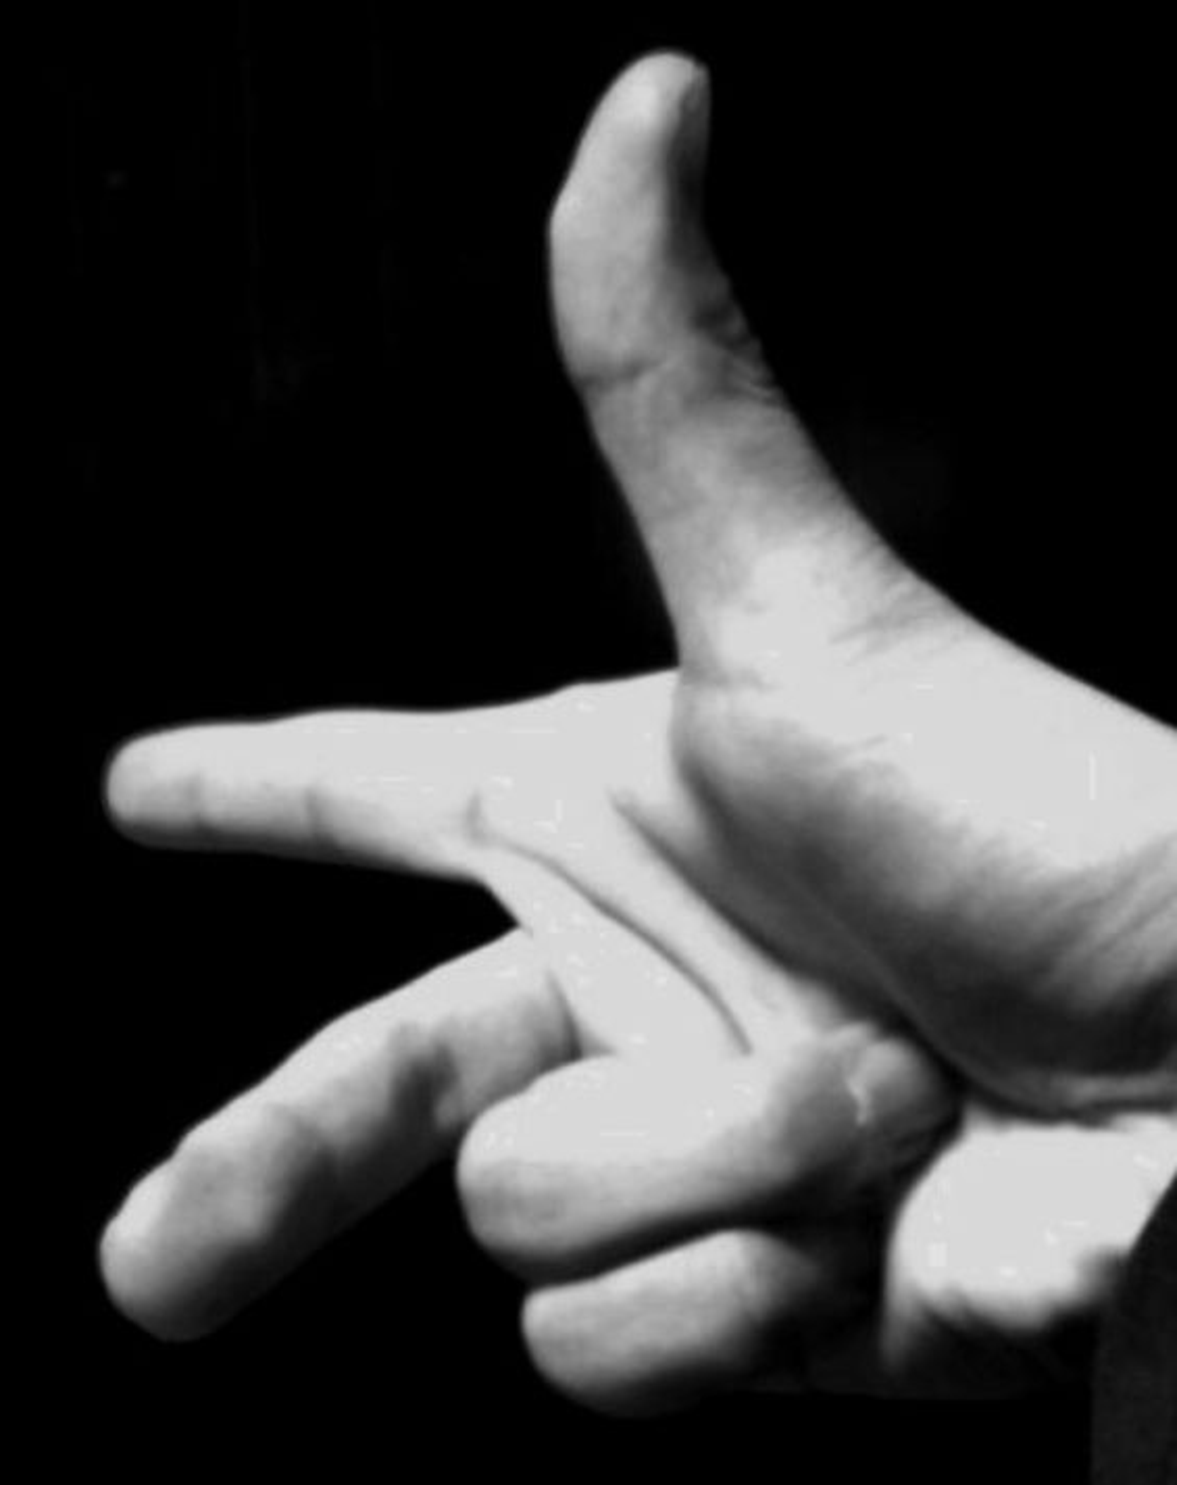
\includegraphics[keepaspectratio, width=3cm,height=3.75cm,clip]{migitekei_TE_mono_x.pdf}

                                    (a) 私の右手
                                    \label{fig:migitekei_TE_mono_x}
                                \end{center}
                            \end{minipage}
                            \begin{minipage}{0.5\hsize}
                                \begin{center}
                                    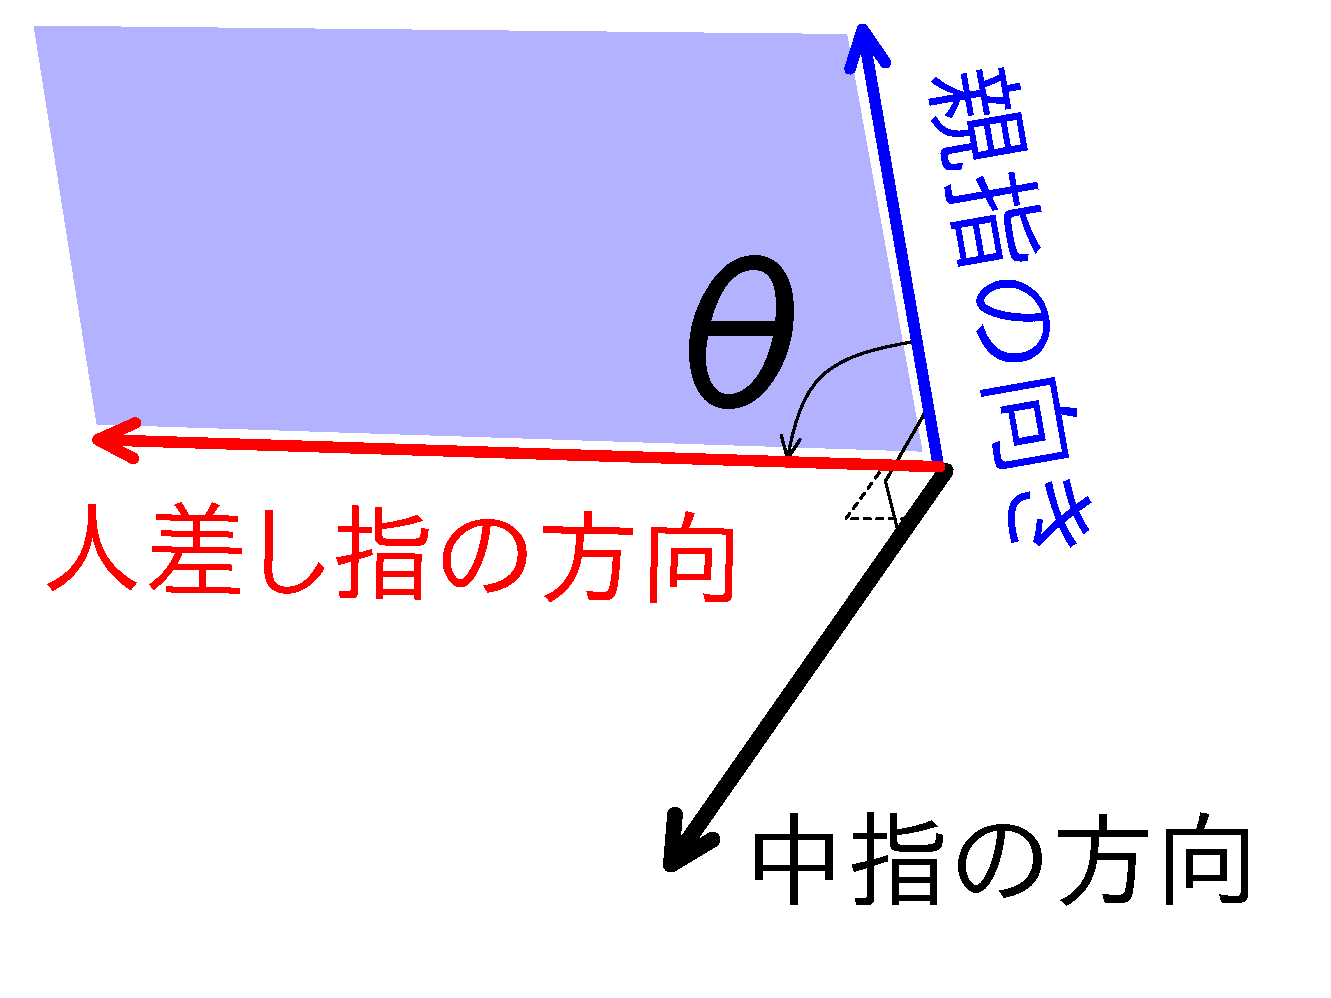
\includegraphics[keepaspectratio, width=3cm,height=3.75cm,clip]{migineji_Myhand.pdf}

                                    (b) 対応図
                                    \label{fig:migineji_Myhand}
                                \end{center}
                            \end{minipage}
                        \end{tabular}
                        \caption{右手系}
                    \end{figure}

                    \begin{figure}[hbt]
                        \begin{center}
                            \includegraphicslarge{VecKagenjoujo.pdf}
                            \caption{ベクトルの和$\cdot$差/$\cdot$積(内積/外積)}
                            \label{fig:VecKagenjoujo}
                        \end{center}
                    \end{figure}
                \end{memo}


%   %==========================================================================
%   %  Section : 特殊なベクトル
%   %==========================================================================
        \section{特殊なベクトル}
%       %----------------------------------------------------------------------
%       %  Input
%       %    File Name : PhysNote_Math_Vector_TaniVector.tex
%       %    説明      : 単位ベクトル,ベクトルの基底などを説明する
%       %----------------------------------------------------------------------
        %   %==========================================================================
%   %  Section : 特殊なベクトル
%   %==========================================================================
        %==================================================================
        %  SubSection
        %==================================================================
            \subsection{単位ベクトル}
                ベクトルは,大きさと向きをもつ.しかし,ベクトルを成分
                表示したときに,その大きさと向きが同時に記述されていて,
                成分表示を見ただけでは,簡単にはその大きさや向きを把握
                することはできない
                    \footnote{
                        計算(暗算)が非常に得意な人や,ベクトルのスペシャリスト
                        でない限り,ベクトルの成分表示を見た瞬間に,その大きさと
                        向きが想像できることはないと思う.少なくとも,私はそのような
                        マネはできない.
                    }.
                そこで,登場するのが,\textbf{単位ベクトル} という概念である.

                自然数でいえば,数字の1がその単位元であり,2以上のすべての自然数は,
                この単位元1の倍数として記述できる.
                    \begin{equation*}
                        2 = 1 \times 2\,,\;3 = 1 \times 3\,,\;\cdots\,.
                    \end{equation*}
                ベクトルの世界では,単位元は1という単なる数値ではなく,
                大きさが1で方向
                    \footnote{
                        「向き」と書いていないことに注意.
                        ここで言っているのは,正の向きと負の向きを同時に
                        考えたいので,「方向」と書いた.
                    }
                をもつ,単位ベクトルという概念が定義される
                    \footnote{
                        定義とは,後の議論の発展のためになされるのであり,
                        導かれるものではない.初学の数学に不慣れである時期には,
                        このことは特に忘れがちである.
                    }.
                    \begin{figure}[hbt]
                        \begin{center}
                            \includegraphicsdefault{TaniVector00.pdf}
                            \caption{単位ベクトル}
                            \label{fig:TaniVector00}
                        \end{center}
                    \end{figure}

                単位ベクトルがあれば,同じ向きを持つベクトルは,その単位ベクトル
                にその大きさをかけることで,ベクトルを表せるのである.
                単位ベクトルと1との違いは,方向をもつか,否かである
                    \footnote{
                        単位ベクトルには方向があり,1には方向がない.
                    }.

                言葉で「単位ベクトル」といったところで,数学的に扱う
                事はできない.なので,単位ベクトルを文字で表そう.

                まだ,単位ベクトルが定義可能か否かは分からないが,
                単位ベクトルなるものがあると仮定して,それを $\bn$ と書くことと
                する.この単位ベクトルを用いると,$\bn$ と同じ方向をもつベクトル
                ならば,$\bn$ の実数倍で表現できる.例えば,ベクトル $\ba$ の向きが
                単位ベクトル $\bn$ と同じ方向であったなら,
                    \begin{equation*}
                        \ba = | \ba | \bn
                    \end{equation*}
                と書ける.これは $\bn$ と同じ向きを持つ任意のベクトルに対して
                成り立つ
                    \footnote{
                        当然,$\bn$ と向きが異るベクトルはこのように記述はできない.
                        その場合には新たに,その方向をもつ別の単位ベクトルを作らないと
                        いけない.つまり,単位ベクトルはその方向によって無数に存在する.
                        これも,自然数の単位元1との違うところだ.
                    }.
                上式を $\bn$ について解くと,
                    \begin{align}
                        \bn = \frac{\ba}{|\ba|}
                    \end{align}
                なる.だから,単位ベクトルとは,ベクトルを自身の大きさで割ったものである
                といえよう.

                念のため,成分表示もしておこう.
                    \begin{align*}
                        \bn &= \frac{\ba}{|\ba|} \\
                            &= \left(
                                    \,\frac{a_{1}}{|\ba|}\,,\,
                                    \,\frac{a_{2}}{|\ba|}\,,\,
                                    \,\frac{a_{3}}{|\ba|}\,\,
                               \right) \\
                            &= \left(
                                    \,\frac{a_{1}}{\sqrt{{a_{1}}^{2}+{a_{2}}^{2}+{a_{3}}^{2}}}\,,\,
                                    \,\frac{a_{2}}{\sqrt{{a_{1}}^{2}+{a_{2}}^{2}+{a_{3}}^{2}}}\,,\,
                                    \,\frac{a_{3}}{\sqrt{{a_{1}}^{2}+{a_{2}}^{2}+{a_{3}}^{2}}}\,\,
                               \right).
                    \end{align*}

                これは大きさが1であり,$\ba$ と同じ方向のベクトルである.なぜなら,ベクトルの
                成分を全てを同じ実数で割ったベクトルと,元のベクトルの方向は同一であることは,
                ベクトルの加減乗除の定義によって簡単に示せる.また,大きさも次の計算から,
                簡単に1であることも確かめられる.
                    \begin{align*}
                        |\bn| &= \left(\frac{a_{1}}{\sqrt{{a_{1}}^2+{a_{2}}^2+{a_{3}}^2}}\right)^{2} +
                                 \left(\frac{a_{2}}{\sqrt{{a_{1}}^2+{a_{2}}^2+{a_{3}}^2}}\right)^{2} \\
                              &\quad + \left(\frac{a_{3}}{\sqrt{{a_{1}}^2+{a_{2}}^2+{a_{3}}^2}}\right)^{2} \\
                              &= \frac{{a_{1}}^{2}+{a_{2}}^{2}+{a_{3}}^{2}}{\left(\sqrt{{a_{1}}^2+{a_{2}}^2+{a_{3}}^2}\right)^{2}} \\
                              &= \frac{{a_{1}}^{2}+{a_{2}}^{2}+{a_{3}}^{2}}{{a_{1}}^2+{a_{2}}^2+{a_{3}}^{2}} \\
                              &= 1 \\
                        \therefore\quad
                        |\bn| &= 1.
                    \end{align*}

                \begin{memo}{具体例}
                    ベクトル $\ba=\left[\,1,\,2,\,4\,\right]$ を,大きさと
                    単位ベクトルに分解してみよう.

                    まず大きさは,定義に従って
                        \begin{equation*}
                            |\ba| = \sqrt{1^{2}+2^{2}+4^{2}} = \sqrt{1+4+16} = \sqrt{21}
                        \end{equation*}
                    である.よって,求めたい単位ベクトルを $\bn$ と書くことにすれば,
                        \begin{equation*}
                            \bn = \frac{\ba}{|\ba|} = \frac{1}{\sqrt{21}}\left[\,1,\,2,\,4\,\right]
                                = \left[
                                    \,\frac{1}{\sqrt{21}},\,\frac{2}{\sqrt{21}},\frac{4}{\sqrt{21}}\,
                                  \right].
                        \end{equation*}

                    以上から,ベクトル $\ba$ は大きさと単位ベクトルに分解すると,
                        \begin{equation*}
                            \ba = |\ba|\bn = \sqrt{21}
                                  \left[
                                    \,\frac{1}{\sqrt{21}},\,\frac{2}{\sqrt{21}},\frac{4}{\sqrt{21}}\,
                                  \right]
                        \end{equation*}
                    と表現される.
                \end{memo}

        %==================================================================
        %  SubSection
        %==================================================================
            \subsection{基底ベクトル}
                先に単位ベクトルという概念を説明した.そして,ここでは
                単位ベクトルを使って,さらに新し考え方を導入する.

                いきなりだけど,具体例から考える.
                ひとつの任意のベクトル $\ba$ を
                もってきて,$\ba$ が次のようなベクトルだったとしよう
                    \footnote{
                        まずは,馴染み深い3次元ベクトルで考える.
                    }.
                    \begin{equation*}
                        \ba
                        =
                        \left[
                            \begin{array}{c}
                                1 \\
                                3 \\
                                5 \\
                            \end{array}
                        \right].
                    \end{equation*}
                この式は次のように見ることもできる.
                    \begin{equation*}
                        \ba
                        =
                        1\left[
                            \begin{array}{c}
                                1 \\
                                0 \\
                                0 \\
                            \end{array}
                        \right]
                        +
                        3\left[
                            \begin{array}{c}
                                0 \\
                                1 \\
                                0 \\
                            \end{array}
                        \right]
                        +
                        5\left[
                            \begin{array}{c}
                                0 \\
                                0 \\
                                1 \\
                            \end{array}
                        \right].
                    \end{equation*}
                3つの方向に対し,ひつの方向に1の大きさをもち,かつ,
                他の方向には0であるような単位ベクトルを作り,
                それに係数をかけて,足し合わせるのである.

                任意のベクトルに対して,この表し方が可能であることは,
                明白である.任意の $n$ 次元ベクトル $\bx$ が
                    \begin{equation*}
                        \bx
                        =
                        \left[
                            \begin{array}{c}
                                x_{1} \\
                                x_{2} \\
                                \vdots \\
                                x_{n} \\
                            \end{array}
                        \right].
                    \end{equation*}
                と成分表示されるとしよう.このとき,$\bx$ は
                次のようにも表現することが可能である.
                    \begin{equation*}
                        \bx
                        =
                        x_{1}\left[
                            \begin{array}{c}
                                1 \\
                                0 \\
                                0 \\
                                0 \\
                                \vdots \\
                                \vdots \\
                                0 \\
                            \end{array}
                        \right]
                        +
                        x_{2}\left[
                            \begin{array}{c}
                                0 \\
                                1 \\
                                0 \\
                                0 \\
                                \vdots \\
                                \vdots \\
                                0 \\
                            \end{array}
                        \right]
                        +
                        \cdots
                        +
                        x_{i}\left[
                            \begin{array}{c}
                                0 \\
                                \vdots \\
                                0 \\
                                1 \\
                                0 \\
                                \vdots \\
                                0 \\
                            \end{array}
                        \right]
                        +
                        \cdots
                        +
                        x_{n}\left[
                            \begin{array}{c}
                                0 \\
                                0 \\
                                0 \\
                                \vdots \\
                                \vdots \\
                                0 \\
                                1 \\
                            \end{array}
                        \right]
                        .
                    \end{equation*}

                    このような書き方だと,記述が少々面倒なので,
                    次のような記号を導入し,表現を簡略化させよう.
                    \begin{align}
                        \be_{1}
                        =
                        \left[
                            \begin{array}{c}
                                1 \\
                                0 \\
                                0 \\
                                0 \\
                                \vdots \\
                                \vdots \\
                                0 \\
                            \end{array}
                        \right]
                        \; , \;
                        \be_{2}
                        =
                        \left[
                            \begin{array}{c}
                                0 \\
                                1 \\
                                0 \\
                                0 \\
                                \vdots \\
                                \vdots \\
                                0 \\
                            \end{array}
                        \right]
                        \; , \cdots , \;
                        \be_{i}
                        =
                        \left[
                            \begin{array}{c}
                                0 \\
                                \vdots \\
                                0 \\
                                1 \\
                                0 \\
                                \vdots \\
                                0 \\
                            \end{array}
                        \right]
                        \; , \cdots , \;
                        \be_{n}
                        =
                        \left[
                            \begin{array}{c}
                                0 \\
                                0 \\
                                0 \\
                                \vdots \\
                                \vdots \\
                                0 \\
                                1 \\
                            \end{array}
                        \right].
                    \end{align}

                    このように,一成分が1であり,他の成分がすべて0であるようなベクトルを,
                    \textbf{基底ベクトル} という.もちろん,基底ベクトルとは,
                    任意のベクトルを表現する場合に用いるベクトルである.しかし,たまたま任意の
                    ベクトルが基底ベクトルの成分と一致してしまうこともある.この場合のベクトルは
                    基底ベクトルとは認識されない.

                    基底ベクトルという概念を使うと,$\bx$ は以下のように書き直せる.
                        \begin{align}
                            \bx = x_{1}\be_{1} + x_{2}\be_{2} + \cdots + x_{i}\be_{i} + \cdots + x_{n}\be_{n}.
                        \end{align}

                    和の記号 $\sum_{i=1}^{n}$ を使うともっと簡単になる.
                        \begin{align}
                            \bx = \sum_{i=1}^{n} x_{i}\be_{i}.
                        \end{align}

                    \begin{memo}{注意}
                        基底ベクトルを先に「一成分が1であり,他の成分がすべて0であるようなベクトル」と
                        定義してしまった.しかし,注意してほしい.より細かく言うと,“直線直交座標系”における
                        基底ベクトルと表現すべきであった.

                        基底ベクトルは,座標系によってことなる.座標系には,直線直交座標意外にも,
                        極座標系や円筒座標系
                            \footnote{
                                後で説明する.中学から使ってきた,$x$--$y$ 座標のことを,直線直交座標というが,
                                これ以外にも,上に書いたように,極座標系や円筒座標系など,様々な座標系を設定
                                できる.ここでは,座標系は直線直交座標系だけではないということを
                                分かってもらえれば,それでいい.
                            }
                        があり,各座標系の基底ベクトルは全く異なるベクトルである
                            \footnote{
                                ただし,ある基底ベクトルが存在するとき,この基底ベクトルを別の基底ベクトル
                                に変換する方法は存在する.
                            }.
                    \end{memo}


\chapter{ベクトル解析}
%   %-----------------------------------------------------------------------------------------------
%   %  Input
%   %    File Name : PhysNote_Math_VctrAnlys.tex
%   %    説明      : 「ベクトル関数」について.考え方と使い方.
%   %-----------------------------------------------------------------------------------------------
        %===================================================================================================
%  Chapter : ベクトル解析
%  説明    : ベクトル解析について説明する.
%===================================================================================================
%   %==========================================================================
%   %  Section
%   %==========================================================================
 \section{ベクトル関数}
    \subsection{ベクトル変数(あるいは,変数ベクトル)}
    ベクトルには,スカラーにおける語彙「変数」に対応する,一般的呼称がない.
    ないと不便なので,このノートでは \textbf{ベクトル変数} という言い方を導入する.
    もしかしたら,\textbf{変数ベクトル} と書くこともあるかもしれない.

    細かいことを言うと,ベクトル変数は,
    成分の一部あるは全部が変数であるようなベクトルであり,
    次に説明するベクトル関数である
        \footnote{
            定義が論理的に循環してしまっているが,意図は伝わるはず.
            循環しないような記述も可能だが,理論構築が目的ではない
            ため,深く突っ込まないでおこう.
        }.

    変数をベクトル変数と区別する意味で,\textbf{スカラー変数} と
    書くこともある.

    \subsection{ベクトル関数}
    ベクトルが絡む関数のことを総称して \textbf{ベクトル関数} という.
    また,ベクトル関数と区別するために,
    今まで考えてきたベクトルが絡まないような関数を,
    \textbf{スカラー関数} と表現する場合がある
        \footnote{
            細かいことを言うと,スカラーは1次元ベクトルだから,
            スカラー関数もベクトル関数である.
        }.

    考えれる例をいくつか上げておこう.特にこれらを区別してよぶ必要は
    ないので,名称を与えることはしない
        \footnote{
            記述の際には,どんな形の
            ベクトル関数について議論している
            かが明確にわかるようにする.
        }.

    例えば,スカラーの独立変数 $t$ に対して,
    1つの定ベクトルが定まる関数が考えられる.これを
        \begin{align}
            \ba (t)
        \end{align}
    と表す.
    関数記号 $\ba$ を太字にした意図は,
    ベクトルが定まる(値域がベクトルである)ことを明示するためである.
    また,$(t)$ という表記は,$t$ が独立変数であることを示すものである
        \footnote{
            多変数になる場合,$\ba(t,\,s)$ と書かれることになる
            ($t$ と $s$ はスカラーである).
            このとき,$(t,\,s)$ という記述がベクトルを成分表示と同じで,
            紛らわしいかもしれない.しかし,文脈により容易に区別できる
            とし,特に書き分けることはしない.この記述の前に関数を
            表現する文字があれば,それらは独立変数である.
        }.

    別の例を上げると,ベクトル変数を独立変数にもつ関数が考えられる.
    数式で表そうとすると,
        \begin{align}
            \ba (\br)
        \end{align}
    のようになる.$\br$ はベクトル変数である.

    上記2つの混合して,スカラー変数 $t$ とベクトル変数 $\br$ から
        \begin{align}
            \ba (t,\,\br)
        \end{align}
    という関数を作ってもいい.

    ベクトル変数を独立変数として,スカラーが定まる(値域がスカラーである)
    関数もあり得る.記号化すれば,
        \begin{align}
            a (\br)
        \end{align}
    となるだろう.関数記号 $a$ を細字にした意図は,スカラーが定まることを
    明示するためである.

    もちろん,スカラー変数 $t$ とベクトル変数 $\br$ をもち,
    スカラーが定まる関数も考えられる.
        \begin{align}
            a (t,\,\br)
        \end{align}

    定ベクトルもベクトル関数の一部として考える.
    明示的な独立変数はないが,入力にかかわらず常に一定値をとるような
    関数として捉える.スカラー関数の場合と同じように考える.

    独立変数が1つのベクトル関数($\ba(t)$)を,\textbf{1変数ベクトル関数} という.
    独立変数が2つ以上のベクトル関数を総称して,\textbf{多変数ベクトル関数} という.
    ベクトル変数をもつベクトル関数($\ba(\br)$ など)は多変数ベクトル関数として考える.

    ひと目で見やすいように,表にしておこう(\Table\ref{table:f4unit}).
        \begin{table}[htb]
          \centering
          \caption{ベクトル関数の種類}
          \begin{tabular}{|l|c|c|l|}                                        \hline
            関数記号      & 独立変数   & 値域     & 例                      \\ \hline  \hline
            $\ba$         & なし       & ベクトル & 定ベクトル              \\ \hline
            $\ba(t)$      & $t$        & ベクトル & ある1点の風向の時間推移 \\ \hline
            $\ba(\br)$    & $\br$      & ベクトル & ある時刻の風向分布      \\ \hline
            $\ba(t, \br)$ & $t$,$\br$ & ベクトル & 風向分布の時間推移      \\ \hline
            $a(\br)$      & $\br$      & スカラー & 風力分布                \\ \hline
            $a(t, \br)$   & $t$,$\br$ & スカラー & 風力分布の時間推移      \\ \hline
          \end{tabular}
          \label{table:f4unit}
        \end{table}

    \subsection{ベクトル関数の微積分}
    \begin{mycomment}
        スカラー関数での微積分を,ベクトル関数へ拡張する.
        ベクトル関数の微積分も,基本的にはスカラー関数と同じように
        計算可能である.
    \end{mycomment}

    \subsubsection{極限}
    ベクトル関数の極限はスカラー関数の場合と同じように定義できる.

    \subsubsection{導関数}

 \subsection{使用用語}
    電磁気学を考えるとき,\textbf{曲線} や,\textbf{閉曲線} 等という数学用語を
    頻繁に使う.ニュートン力学では,特に必要はない
        \footnote{
            知っていれば,それだけ“広く”考えられるが,
            無理してまで,ここで学習する必要はない.
        }.
    だから,電磁気学を学習し始める段階になったら,この部分を読むようにすればいい.

    最初に,これらの用語について,あらかじめ
    確認する.以下の説明はすごく感覚的なものであって,
    全く厳密でないことを注意しておく.

 \subsubsection{導線(曲線)}
    一本のひものように,端と端が結ばれていない線のことを 曲線 という.
    このノートでは,「電気の流れる道」という意味をこめて,\textbf{導線} と
    いうことにする.導線の形は グニャグニャ と曲がっていてかまわないが,
    導線が自身と重ならないようなものであるとする(リボンのように絡まっていないものする).
    このノートでは,導線を表現する記号として,$\Gamma$ を用いる.
                \begin{figure}[hbt]
                    \begin{center}
                        \includegraphicslarge{kyokusenn.pdf}
                        \caption{導線}
                        \label{fig:kyokusenn}
                    \end{center}
                \end{figure}

    数学的に表現すると,曲線とは各成分が共通のパラメータ $t$ の
    関数であるようなベクトルのことをいう.式で表せば,曲線 $\br(t)$ は
        \begin{align}
            \br_{n}(t)=\left( x_{1}(t),\,x_{2}(t),\,x_{3}(t),\cdots ,\,x_{n}(t)\right)
        \end{align}
    と書ける.これは $n$ 次元ベクトルである.
    このノートでは空間の次元である3次元を考えているので,その各成分は $\left(x(t),\,y(t),\,z(t)\right)$ と書くことにし,
        \begin{align}
            \br(t)=\left( x(t),\,y(t),\,z(t)\right)
        \end{align}
    とする.この式は時刻 $t$ における位置を表現する式と同じである.時間 $t$ を正方向に
    なめらかに変化させていき,その各々の時間における位置を記録していけば,1つの曲線が現れてくる.
    力学ではこの曲線のことを「軌跡」とよんでいたが,ここではそれを一般的に解釈して,\textbf{曲線} と
    いうことにする.このノートの電磁気学の部分においては,曲線として出てくるのは回路の導線である.そこで,曲線とよばずに,
    \textbf{導線} ということが多い.また,導線の形をいちいち指定することはしない.だから,$\Gamma=\br(t)$ として,
    導線を表現する記号として,$\Gamma$ を用いる.

    以下では導線は連続しているという条件を課する.簡単にいえば,「切れていない」導線を考えるということである.

 \subsubsection{閉曲線}
    導線の両端がつながっているとき
    \footnote{
        この場合,どこが端であるかは見分けがつかないが….
    }
    ,これを \textbf{閉曲線} という.
    閉曲線の形は    グニャグニャ と曲がっていてもよいが,
    「八の字」のように導線同士が接触してが重ならないようにする.
    輪ゴムのようなものを考えるとよい.
    このノートでは,閉曲線を表現する記号として,$l$ を用いる.

                \begin{figure}[hbt]
                    \begin{center}
                        \includegraphicsdefault{heikyokusenn.pdf}
                        \caption{閉曲線}
                        \label{fig:heikyokusenn}
                    \end{center}
                \end{figure}

 \subsubsection{曲面}
    平らではなく,  グニャグニャ とした面のことを \textbf{曲面} という.
    もちろん,平らな面も曲面に属するが,ここではもっと一般的なグニャッと
    なった面を想像してもらいたい.

    電磁気学では特に,「縁をもった曲面」を考えることも多い
        \footnote{
        例えば,お皿等がその例になるだろう.
        縁を持たない曲面の例とは,ボールの表面があげられよう.
        }.
    曲面の境界は
    閉曲線である.従って以下では,「縁をもった曲面」のことを
    『閉曲線 $l$ を縁とする曲面』
    のようにいうことにする.
    このノートでは,閉曲線 $l$ を縁とする曲面 を 表現する記号として,
    $S_{l}$ を用いることにする.

 \subsubsection{閉曲面}
    ボールの表面のように,縁をもたない曲面のことを \textbf{閉曲面} という.
    グニャグニャとしていてよいが,面同士が重なったり,互いに切断しあったりしない
    ものとする.    このノートでは,閉曲面を表現する記号として,$S$ を用いる.

    ここで
    注意したい,「閉曲線 $l$ を縁とする閉曲面 $S_{l}$」と「閉曲線 $S$」の違いである.
    $S$ の添え字に $l$ が付いているもの($S_{l}$)は曲面であり,
    添え字に $l$ がついていないもの($S$)は閉曲面である.
                \begin{figure}[hbt]
                    \begin{tabular}{cc}
                        \begin{minipage}{0.5\hsize}
                    \begin{center}
                        \includegraphicsdouble{kyokumenn.pdf}
                        \caption{曲面}
                        \label{fig:kyokumenn}
                    \end{center}
                        \end{minipage}
                        \begin{minipage}{0.5\hsize}
                    \begin{center}
                        \includegraphicsdouble{heikyokumenn.pdf}
                        \caption{閉曲面}
                        \label{fig:heikyokumenn}
                    \end{center}
                        \end{minipage}
                    \end{tabular}
                \end{figure}

 \subsubsection{領域}
    閉曲面 $S$ を考えるとき,その表面は その内側の空間 と 外側の空間 を分けていると
    考えられる.閉曲面の内側の空間のことを \textbf{領域} という.
    領域を表現する記号として,このノートでは $\Omega_{S}$ を用いる.もちろん,
    添え字の $S$ は領域の表面である閉曲面 $S$ を意味している.
                \begin{figure}[hbt]
                    \begin{center}
                        \includegraphicsdefault{ryouiki.pdf}
                        \caption{領域}
                        \label{fig:ryoiki}
                    \end{center}
                \end{figure}

 \subsection{線積分と面積分のイメージ}
    \begin{quotation}\small
    線積分と面積分についての詳しいことは,
    ベクトル解析の教科書や微分積分学の教科書
    を参照してもらうことにして,ここではそのイメージを
    記述しておく.
    \end{quotation}

 \subsection{ベクトル空間}
    位置を一つ指定すると,その位置に対して,
    1つのベクトルが指定される空間を考える(図\ref{fig:vector_sp}参照).
                \begin{figure}[hbt]
                    \begin{tabular}{cc}
                        \begin{minipage}{0.5\hsize}
                            \begin{center}
                                \includegraphicslarge{vector_sp.pdf}
                                \caption{ベクトル空間1(説明図)}
                                \label{fig:vector_sp}
                            \end{center}
                        \end{minipage}
                        \begin{minipage}{0.5\hsize}
                                \begin{center}
                                \includegraphicslarge{vector_sp2.pdf}
                                \caption{ベクトル空間2(イメージ)}
                                \label{fig:vector_sp2}
                            \end{center}
                        \end{minipage}
                    \end{tabular}
                \end{figure}

    任意の位置 $\br$ に対して,
    1つのベクトル $\bA$ が
    決定されるという空間をイメージして描いた図である.
    このような空間を \textbf{ベクトル空間} という.
    また,位置(と時間)を指定すると
    1つのベクトルを決定できるので,
    これは関数の性質に他ならず,
    これを \textbf{ベクトル関数} という.
    従って,$\bA$ を $\bA(\br)$ と
    表現したほうがベクトル関数であることが,明確になる.
    しかし今後も,式が煩雑にならないように,
    ベクトル関数の変数である $\br$ を
    省略して表現する($\bA:=\bA(\br)$).

    ベクトル空間の例としてよく取り上げられる現象のうち,
    空気の流れ(風)がある.風は向きと速度をもっている.
    その向きと速度は場所と時間によって異なるが,
    1つの場所と時間を指定すれば,風の向きと速度は
    求まる.
    川の流れや,海水の流れといった現象も
    ベクトル空間で表現される.要するに,
    何かの「流れ」があったときに,
    それはベクトル空間で表現するのである.

    以下でベクトル空間というときには,図\ref{fig:vector_sp2}
    を思い浮かべてもらいたい.但し,
    ベクトル $\bA$ については,
    時間と位置を指定すれば決定されるようなものであれば,
    図\ref{fig:vector_sp2}のようなものでなくとも,自由に想像してよい.



 \subsection{ベクトルとスカラーの区別の仕方}
                いままで,ベクトルとは大きさと向きのある量であると
                考えてきた.また,スカラーは大きさのみをもつ量とし
                ていた.実は,これは正確な説明ではない.ベクトル空間を
                確認した今,ベクトルとスカラーの正確に違いについて,
                議論ができる.ここで整理しよう.

                ベクトルとスカラーを正確に区別する方法は,座標変換を
                考えることである.私がある空間に直交座標を張ったとしよう.
                私のいる空間には,複数の人がいて,その各々が任意に
                直交座標を張るとする.もちろん,何人もの人が張った直交
                座標の座標軸の方向はばらばらである.

                この空間が,ベクトル空間であったとしよう.その時,私は
                1つの点に属する1つのベクトルをみるとする.
                そのベクトルの方向は,私から見た方向と,他の観測者から見た
                方向とで一致しない
                    \footnote{
                        偶然の一致は起こりえるが,より一般的に考えよう.
                    }.
                それでは,この空間がベクトル空間ではなく,スカラー空間であるとしよう.
                この時には私がさしている点に属する数は,別の観測者が
                それを見ても,全く一致する.ベクトルとスカラーの違いは
                ここにある.私が見るベクトルの向きと,他の人が同じベクトルを見たときの
                むきは異なるが,スカラーは度の観測者に対しても同じ値を示す.
                観測者によって違うということは,直交座標の座標軸の設定方向が違う
                ということである.つまり,別の座標に移ってしまうと,ベクトルの向きは
                変化してしまうのである.スカラーは座標が変わっても,全く同じように
                観測される.両者はこのように,座標変換によって区別されるものである.
                座標変換についての知識がないので,これ以上ここでは話を続けることができない.
                座標変換について学ぶときに,もう一度,
                ベクトルとスカラーの違いを確認し,“実感”したいと思う.ここでは
                区別の仕方が知識として身に付いていれば,それでよいことにしよう.


 \subsection{線積分}
    ベクトル空間に,任意の曲線 $C$ を描く.
    この曲線 $C$ 上の全ての点にはそれぞれ1つの
    ベクトルが対応している.ベクトル空間に
    曲線 $C$ を描いてみると図\ref{fig:sensekibun}のようになる.
                \begin{figure}[hbt]
                    \begin{center}
                        \includegraphicslarge{sensekibun.pdf}
                        \caption{線積分}
                        \label{fig:sensekibun}
                    \end{center}
                \end{figure}


    見易さのために,曲線 $C$ 上のベクトルしか描いていないが,
    実際は別の点においてもベクトルは存在している.
    線積分の考察の対象はあくまでも,曲線 $C$ 上のベクトルだけである.

    曲線 $C$ を微小な長さの直線分割して,そのひとつひとつを $\df l$ とする.
    この部分の単位接線ベクトルを $\bt$ で表現する.
    もちろん,曲線 $C$ は曲がっているので,各 $\df l$ 部分における
    単位接線ベクトル $\bt$ は一定ではない.
    これらにより,長さ $\df l$ で向きが $\bt$ である
    ベクトル $\bt\,\df l$ を曲線 $C$ 上に
    作ることができる.$C$ 上に位置するベクトル $\bA$ の
    接線方向は  $\bA\cdot\bt\,\df l$ と
    表現できる.これを曲線 $C$ 全域にわたって積分したものが,
    線積分であり,
        \begin{align}
        \int_{C} \bA\cdot \bt\df l
        \end{align}
    と表現される.

    曲線 $C$ 上のベクトル $\bA$ の曲線方向成分 $\bt$ の
    積分を表している.


    \begin{memo}{詳細}
        もう少し優しく解説してみる.線積分とは,曲線 $C$ 上のベクトル関数を
        ,曲線 $C$ に沿って積分するということである.
        「曲線 $C$ に沿って積分する」というのは,ベクトル関数の曲線方向成分の
        総和を考えるということである.そのためには,曲線 $C$ とその上のベクトル $\bA$ の
        内積を考える必要がある
        \footnote{
        任意の2つのベクトル $\textit{\textbf{u}}$,$\bv$ の
        内積は $\textit{\textbf{u}}\cdot\bv=uv\cos\theta$ である.
        }
        すなわち,曲線をベクトルとしてみることが要求され,曲線に向きをつけるということである.
        曲線の向きは2通り考えられるが
        \footnote{
        曲線の両端をそれぞれA,Bとして,まず第1にAからBに向かう向きを考えられる.
        また,第2に,BからAに向かう向きを考えられる.
        }
        ,どちらをとろうが,結果は同じである.しかし,一度向きを指定したら,
        後になって変更することはできない.

        曲線 $C$ を有限の $N$ 個に分割しする(\ref{fig:senseki2}参照).
        このように分割された曲線は,ほとんど直線と見ることができる.
        つまり,曲線 $C$ を $N$ 個の直線で近似するのである.
        これらの近似的直線に名前と番号をつけて $\Delta l_{1}$,$\Delta l_{2}$,…,$\Delta l_{N}$ とする.
        また,これらに向きという概念を導入して,それぞれに $\bt_{1}$,
        $\bt_{2}$,…,$\bt_{N}$ を対応させる.
        もちろん,先ほど決めた曲線の向きに合うように設定する.
        そして,
        $\bt_{1}\Delta l_{1}$,$\bt_{2}\Delta l_{2}$,
        …,$\bt_{N}\Delta l_{N}$ を作る.
        これらのベクトルは曲線の接線の向きを持ち,大きさが $\Delta l$ である
        \footnote{
        \textbf{単位ベクトル};
        任意のベクトル $\bv$ を用意する.ここで,
        大きさ1の向きを持った \textbf{単位ベクトル} を導入し,
        これを $\textit{\textbf{m}}$ と書く.
        この単位ベクトル $\textit{\textbf{m}}$ を用いて
        任意のベクトル $\bv$ はその大きさを $v$ と
        表すことで,
        \begin{align}
         \bv=v\textit{\textbf{m}}
        \end{align}
        と書ける.ここでは $\bv$ が曲線に沿うベクトルに対応し,
        $v$ はその大きさ $\df l$,$\textit{\textbf{m}}$ は向き$\bt$に対応している.
        }
        .

        ところで,この分割に際して,$C$ 上のベクトル $\bA$ は
        連続であるために,分割した直線部分には複数のベクトルが含まれることになる.
        そこで,ベクトル $\bA$ を
        1つの直線で平均して,それぞれ,$\bA_{1}$,
        $\bA_{2}$,…,$\bA_{N}$ とする.
                    \begin{figure}[hbt]
                        \begin{center}
                            \includegraphicsdefault{senseki2.pdf}
                            \caption{線積分(説明図)}
                            \label{fig:senseki2}
                        \end{center}
                    \end{figure}

        以上より,曲線 $C$ 上のベクトルと
        曲線に沿ったベクトルとの内積の和は
        \begin{align}
        \bA_{1}\cdot\bt_{1}\Delta l_{1}
        +\bA_{2}\cdot\bt_{2}\Delta l_{2}
        +\cdots
        +\bA_{N}\cdot\bt_{N}\Delta l_{N}
        \end{align}
        和の記号 $\displaystyle\sum$ を用いて表現すれば,
        \begin{align}
        \sum_{i=n}^{N}\bA_{i}\cdot\bt_{i}\Delta l_{i}
        \end{align}
        さらに分割数 $N$ を無限大に持ってことで,曲線に近づいていき,最終的には
        \begin{align}
        \lim_{N\to\infty}\sum_{i=n}^{N}\bA_{i}\cdot\bt_{i}\Delta l_{i}
        =\int_{C} \bA\cdot \bt\df l
        \end{align}
        を得る.
    \end{memo}

 \subsection{面積分}
        ベクトル空間に,
        任意の閉曲面 $S$ を
        とる(図\ref{fig:mensekib}参照).
                \begin{figure}[hbt]
                    \begin{tabular}{cc}
                        \begin{minipage}{0.5\hsize}
                    \begin{center}
                        \includegraphicsdouble{mensekibun1.pdf}
                        \caption{面積分(巨視的視点から)}
                        \label{fig:mensekib}
                    \end{center}
                        \end{minipage}
                        \begin{minipage}{0.5\hsize}
                    \begin{center}
                        \includegraphicsdouble{mennsekibunnbisi.pdf}
                        \caption{面積分(微視的視点から)}
                        \label{fig:mennsekibunnsbisi}
                    \end{center}
                        \end{minipage}
                    \end{tabular}
                \end{figure}


        曲面 $S_{l}$ の各点から,流出するベクトルを考える.
        曲面 $S_{l}$ 上の位置 $\br$ から
        流出するベクトルを $\bA$ とする.

        曲面 $S_{l}$ を無限に分割し,その微小面積部分のひとつひとつを $\df S_{l}$ と表す.
        曲面 $S_{l}$ から流出するベクトルの垂直な成分が,実質的に流出する量である.
        曲面 $S_{l}$ に平行な成分は曲面 $S_{l}$ 上を流れるだけであり,流出はしない.
        そこで,曲面 $S_{l}$ に垂直な成分を考えるために,曲面 $S_{l}$ と
        流出するベクトル $\bA$ の内積を考える必要が生じる.つまり,
        曲面 $S_{l}$ をベクトルとして考えることになる.そのままでは
        ベクトルにすることができないので,線積分のときと同様に,
        単位ベクトルの導入をする.線積分のときは曲線に沿うベクトルにしたかったので
        単位接線ベクトルを考えたが,面積分では曲面 $S_{l}$ に垂直な
        方向を考えたいので,\textbf{単位法線ベクトル} を導入し,これを $\textit{\textbf{n}}$ とする.
        さて,どのような向きに設定するかだが,
        曲面には2つの面が考えられる.すなわち裏と表を考えられる.従って,
        単位法線ベクトルの向きとして「裏から表」と「表から裏」の2つの向きのどちらか一方を
        つける必要がある.しかし明らかに,どちらの向きにとろうが結果は同じである.
        一度向きを決定したら,後になってその向きを変更してはいけない.

        このように設定した単位法線ベクトルを用いて,曲面の各微小面積部分 $\df S$ における
        ベクトルは,$\textit{\textbf{n}}\df S$ と書ける.というか,こういう概念を導入するのである.
        このベクトルの大きさは $\df S$ であり,
        向きは法線ベクトルの向きである.

        以上によって,微小面積部分 $\df S$ から流出するベクトル $\bA$ は,$\textit{\textbf{n}}\df S$ と
        の内積から $\bA\cdot\textit{\textbf{n}}\df S$ と表現できる.曲面 $S_{l}$ 全体を
        考えるならば曲面で積分すればよく,
        \begin{align}
        \int_{S_{l}} \bA\cdot \textit{\textbf{n}}\df S_{l}
        \end{align}
        である.

        式のイメージは,曲面 $S_{l}$ から流出するベクトルの
        総和である.どのくらいの量が流出しているかを
        計算するのがこの式である.

        微分形のマクスウェル方程式を得るために必要な概念は
        ベクトルの \textbf{発散}($\rm{div}$)と,
        ベクトルの \textbf{回転}($\rm{rot}$)である.
        まずは,この2つについて確認する.
        さらに今後必要となるベクトル解析の公式もここに書き下しておく.


 \subsection{ベクトルの発散・回転・勾配}


 \subsubsection{ベクトルの発散($\rm{div}$)}
        ベクトルの発散というのは,ある点でベクトルの「湧き出し」が生じているかどうかを表現する
            \footnote{
            湧き出しのことをdivergenceというので,その頭文字$\rm{div}$をとって,
            これを発散の数式記号として用いる.
            }.
        もしその値が正であれば,その点でベクトルが湧き出ているのであり,
        負であれば吸収が起こっていることを意味する.

        ベクトルの発散の計算方法なのだけど,ここでは厳密なことは考えず,
        感覚的な説明にとどめる
            \footnote{
                もし,より厳密に知りたければ,
                「ベクトル解析」の教科書にあたってみるとよい.
            }.
        ベクトルといってもイメージがわきにくいので,
        ここでは水の流れ(川)を例にとって説明したい.
        水の流れのベクトルを $\bA(\br)$ で表すことにする.

        ある点Pで水が湧き出ているとき,正方形の箱でその点Pを
        内部に含むように囲む.
                \begin{figure}[hbt]
                    \begin{center}
                        \includegraphicsdefault{div1.pdf}
                        \caption{発散のイメージ}
                        \label{fig:div1}
                    \end{center}
                \end{figure}

        もし,Pから水が湧き出していないのなら,この箱に
        入ってくる水の量と,箱の外に出て行く水の量の和は0である.
        ここで,この箱は正方形であるから,水が流入する面と
        流出する面はそれぞれ3面ずつである.そこで,向かい合う
        面同士の対をつくり,一方の面から水が流入し,
        その面の向かい側の面から水が流出するという状況を
        考える.もちろん,3つの組が作られるが,ここでは説明を簡単にするために,
        1組の面を考える.
                \begin{figure}[hbt]
                    \begin{center}
                        \includegraphicsdefault{div00.pdf}
                        \caption{湧き出し(一方向)}
                        \label{fig:div00}
                    \end{center}
                \end{figure}

        図\ref{fig:div00}において,
        水が流入する面の面積は,$\Delta y\Delta z$ であることは
        図より明らか.従って,この面に流入する水の量は,
            \begin{equation*}
                A_{x}(x, y, z)\Delta y\Delta z
            \end{equation*}
        である.また,流出する水の量は,
            \begin{equation*}
                A_{x}(x+\Delta x, y, z)\Delta y\Delta z
            \end{equation*}
        である.湧き出しの量は,流入する水の量から流出する量を
        引けばよい.従って,
            \begin{equation*}
                A_{x}(x+\Delta x, y, z)\Delta y\Delta z-A_{x}(x, y, z)\Delta y\Delta z
            \end{equation*}
            \begin{equation*}
                \Leftrightarrow \quad \{ A_{x}(x+\Delta x, y, z)-A_{x}(x, y, z)\}\Delta y\Delta z
            \end{equation*}
        と計算される.ここで,
        $A_{x}(x+\Delta x, y, z)-A_{x}(x, y, z)=(\rd A_{x}/\rd x)\Delta x$ であることに
        注意すれば
            \footnote{
                $\Delta x$の2次以上の項は無視した.
            }
            \begin{equation*}
                \Leftrightarrow \quad  \frac{\rd A_{x}}{\rd x}\Delta x\Delta y\Delta z
            \end{equation*}
        となる.これは正か負の値をもつ.
        正の場合は湧き出しが起こっていることを意味し,
        負の場合は吸収が起こっていることを意味する.

        これは他の2組の面においても同様に計算でき,
        結果を記しておけば,
            \begin{equation*}
                \frac{\rd A_{y}}{\rd y}\Delta x\Delta y\Delta z, \qquad
                \frac{\rd A_{z}}{\rd z}\Delta x\Delta y\Delta z
            \end{equation*}
        である.

        以上から,正方形の箱から流れ出す量は,それぞれの和を考えればよく,
            \begin{equation*}
                \frac{\rd A_{x}}{\rd x}\Delta x\Delta y\Delta z
                +\frac{\rd A_{y}}{\rd y}\Delta x\Delta y\Delta z
                +\frac{\rd A_{z}}{\rd z}\Delta x\Delta y\Delta z
            \end{equation*}
            \begin{equation*}
                \Leftrightarrow \quad
                \left(
                \frac{\rd A_{x}}{\rd x}
                +\frac{\rd A_{y}}{\rd y}
                +\frac{\rd A_{z}}{\rd z}
                \right)
                \,\Delta V
            \end{equation*}
        である.ここに,$\Delta V=\Delta x\Delta y\Delta z$ とした.これは
        箱の体積を表すものである.

        ここで,ベクトル $\bA=(A_{x},\, A_{y},\, A_{z})$ の
        発散 $\ddiv$ は次式で定義される.\\
        \begin{itembox}[l]{発散( $\ddiv$ )の定義}
            \begin{align}
                \mathrm{div\,}\bA:=
                \frac{\rd A_{x}}{\rd x}+
                \frac{\rd A_{y}}{\rd y}+
                \frac{\rd A_{z}}{\rd z}
            \end{align}
        \end{itembox}\\

        この発散記号 $\ddiv$ を用いると,
            \begin{align}
                \mathrm{div\,}\bA\,\Delta V
            \end{align}
        となる.これを体積 $\Delta V$ で割ると,
        単位体積あたりの湧き出しの量を計算できる.
            \begin{align}
                \frac{1}{\Delta V}\mathrm{div\,}\bA\,\Delta V
            \end{align}
        箱の内部で湧き出した分だけ,水は
        この箱の外に流出するが,
        この関係について次の項目で考える.




 \subsubsection{ガウスの定理}

        前項目での箱の体積,つまり $\Delta V$ を極限まで小さくしていき,それをある領域で
        積分する.この領域をつぎのように設定する.閉曲面 $S$ をとり,その内側の領域を $\Omega_{S}$  とする.
        また,この領域の体積を $V$ とする.そして,まず体積 $V$ を分割して $\Delta V$ とする.
        この $\Delta V$ を領域 $\Omega_{S}$ で積分するということは,以下の通りに計算するということである.
            \begin{equation*}
                \lim_{\Delta V \to \infty}\left(\frac{1}{\Delta V}\sum\mathrm{div\,}\bA\,\Delta V\right)
            \end{equation*}
        積分記号を用いれば,
            \begin{align}\label{divA1}
                \int_{\Omega_{S}} \mathrm{div\,}\bA\,\df V
            \end{align}
        である.この積分は,領域 $\Omega_{S}$ からの湧き出しの量を計算するものである.

        ところで,
        領域 $\Omega_{S}$ から湧き出した量は領域内にとどまれず,
        外にあふれてしまうはず.つまり,湧き出した分だけ,領域の表面である閉曲面 $S$ を
        貫いて領域外へともれてしまう.閉曲面 $S$ から流れ出る量は,
            \begin{align}\label{intS_A_dS}
                \int_{S} \bA \cdot \textit{\textbf{n}}\,\df S
            \end{align}
        と計算できる.

        従って,“湧き出した分だけ流出する”ことを式で表現するならば,式(\ref{divA1})と式(る)が
        等しいとするべきで,
        すなわち,
            \begin{align}
                \int_{\Omega_{S}} \mathrm{div\,}\bA\,\df V=\int_{S} \bA \cdot \textit{\textbf{n}}\,\df S
            \end{align}
        が成立している.これを \textbf{ガウスの定理} という.
        左辺が体積積分で,右辺が面積分になっている面白い定理である.
                \begin{figure}[hbt]
                    \begin{center}
                        \includegraphicsdefault{int_gauss_law1.pdf}
                        \caption{ガウスの定理(イメージ)}
                        \label{fig:int_gauss_law1}
                    \end{center}
                \end{figure}


        ガウスの定理を感覚的に説明してしまったが,
        これは数学的には厳密に証明されるべき定理である.
        このノートではこの定理の証明はしないが,
        この定理は大事なものだから,
        ベクトル解析の教科書を読んで,証明を
        確認するとよい.
        ここでは,この定理の直感的な理解と扱い方がわかれば,それでよいことにしたい.

        \begin{memo}{整理}
           もう一度整理しよう.
           任意の閉曲面を $S$,この閉曲面 $S$ の内側の領域を $\Omega_{S}$ と表す.
           また,閉曲面の単位法線ベクトルを $\textit{\textbf{n}}$ 表す.このとき,
           任意の3次元ベクトル $\bA$ に対して以下の関係が成り立つ.\\
           \begin{itembox}[l]{ガウスの定理}
               \begin{align}
                   \int_{\Omega_{S}} \ddiv \bA\,\df V
                   =\int_{S} \bA\cdot\textit{\textbf{n}}\,\df S
               \end{align}
           \end{itembox}\\

           言葉で式を表現するならば
               \begin{equation*}
                   \mbox{(領域内での湧き出し量)}=\mbox{(領域外への流出量)}
               \end{equation*}
           といった感じだろうか.
        \end{memo}

        \begin{memo}{「ガウスの法則」と「ガウスの定理」}
           “ガウスの法則”との区別をしっかりしておくこと.
           \begin{itemize}
               \item ガウスの法則は電場や磁束密度の振る舞いを表す "物理法則"
               \item ガウスの定理とはベクトルの発散に関する "数学の定理"
           \end{itemize}
        \end{memo}

        \subsubsection{ベクトルの回転($\rm{rot}$)}
        ベクトルの回転
        を式で表現することを考える
            \footnote{
                回転のことをrotationというので,その頭文字のrotが
                数式記号として用いられる.
            }.

        ベクトルの回転とは,1つのベクトルが時間的に向きを変えて変化するような回転ではない.
        ベクトル空間自体が回転運動をしているのでもない.
        どのようなことか.具体例で考えよう.

        ここでも,具体的なベクトルの例として水の流れ(川)を用いる.
        川を見ると,岩や石の付近で“渦”を巻いている所があるだろう.
        これから考えることは,この“渦”を数式で表現することである.
                \begin{figure}[hbt]
                    \begin{center}
                        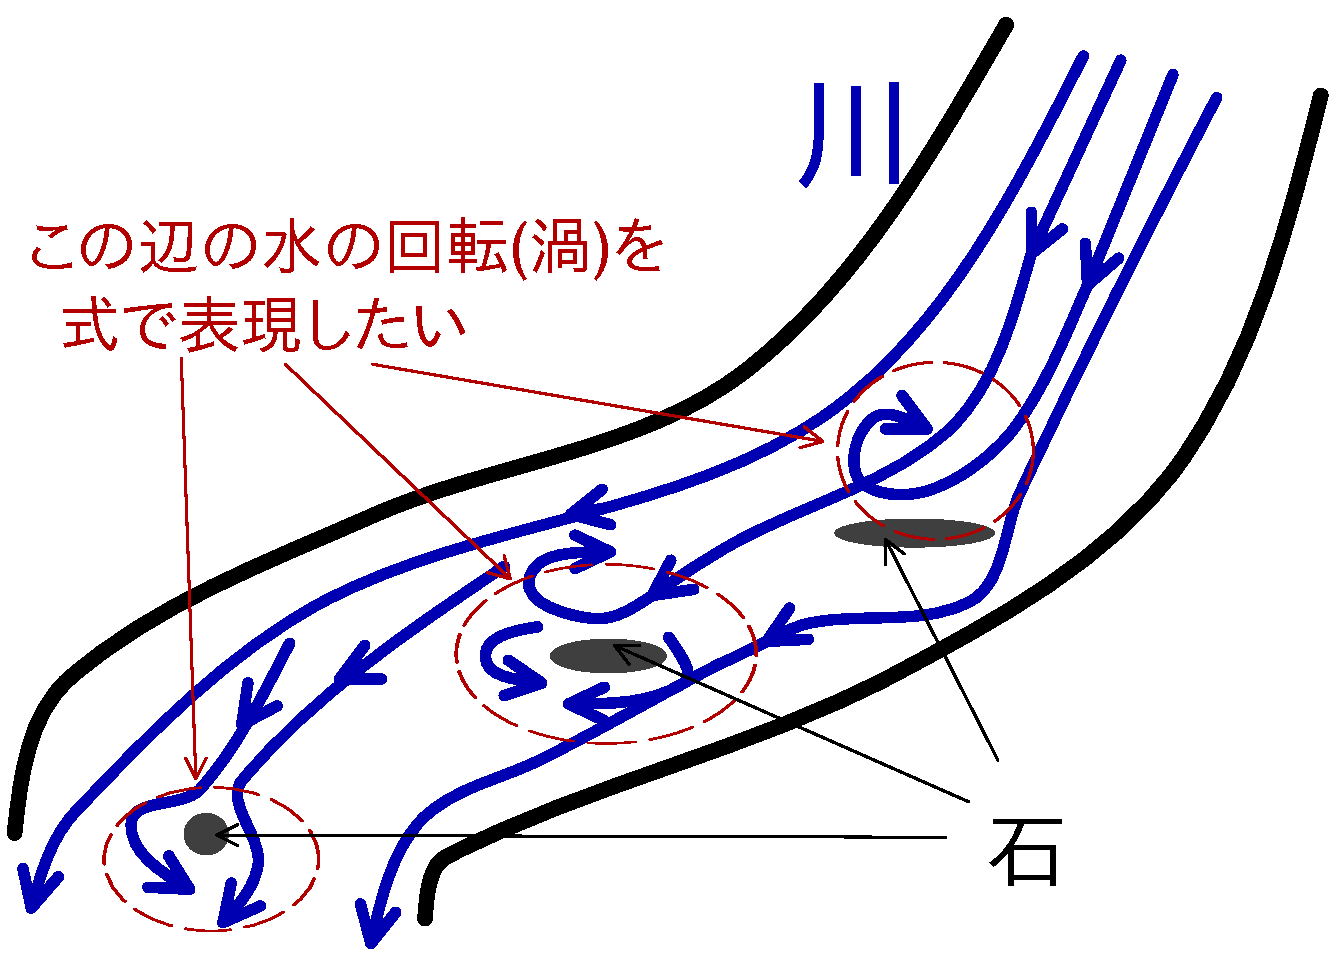
\includegraphics[keepaspectratio, width=4cm,height=2.87cm,clip]{image_rot_1.pdf}
                        \caption{川で生じる渦のイメージ}
                        \label{fig:image_rot_1}
                    \end{center}
                \end{figure}

        物体の回転を扱ったときは,直接的に物体そのものの運動を
        考えることができた.ところが,水などの流体は物体とは異なり,
        その流れ自体を物体と同じように考えるとややこしい.
        そこで,どのような流れかを知るために,川の上に
        葉を置いてみるのだ.葉は,水の流れに従って移動する.
        この葉の動きを観察することにより,
        川の様子を探ることができる.川の全体の
        様子を把握したい場合には,その川のいたるところに
        葉を置いて見て,その葉がどのような動きをするかを,
        観察すればよい.

        葉が1つの場所にとどまっていて,その場で
        回転している状況を想定する.この回転面に $x-y$ 面をとる
            \footnote{
                これは葉が置かれている表面,つまり水面に $x-y$ にとるのと同じである.
            }.
        そして,葉が回転している一点を原点にとる.
                \begin{figure}[hbt]
                    \begin{tabular}{cc}
                        \begin{minipage}{0.5\hsize}
                    \begin{center}
                        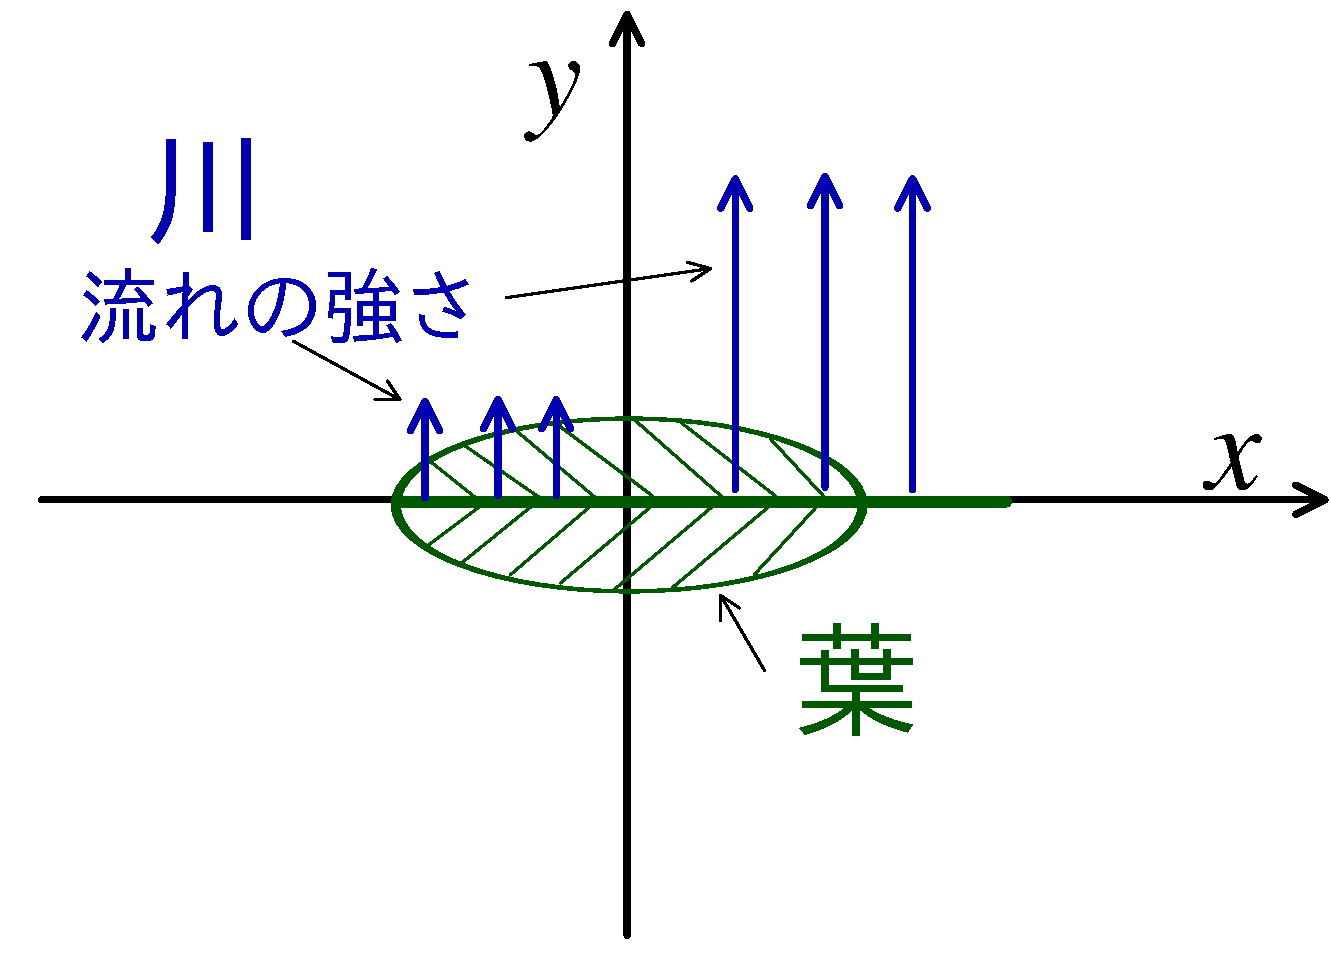
\includegraphics[keepaspectratio, width=4cm,height=2.87cm,clip]{rotrotrot.pdf}
                        \caption{回転(渦)が生じるための条件}
                        \label{fig:rotrotrot}
                    \end{center}
                        \end{minipage}
                        \begin{minipage}{0.5\hsize}
                    \begin{center}
                        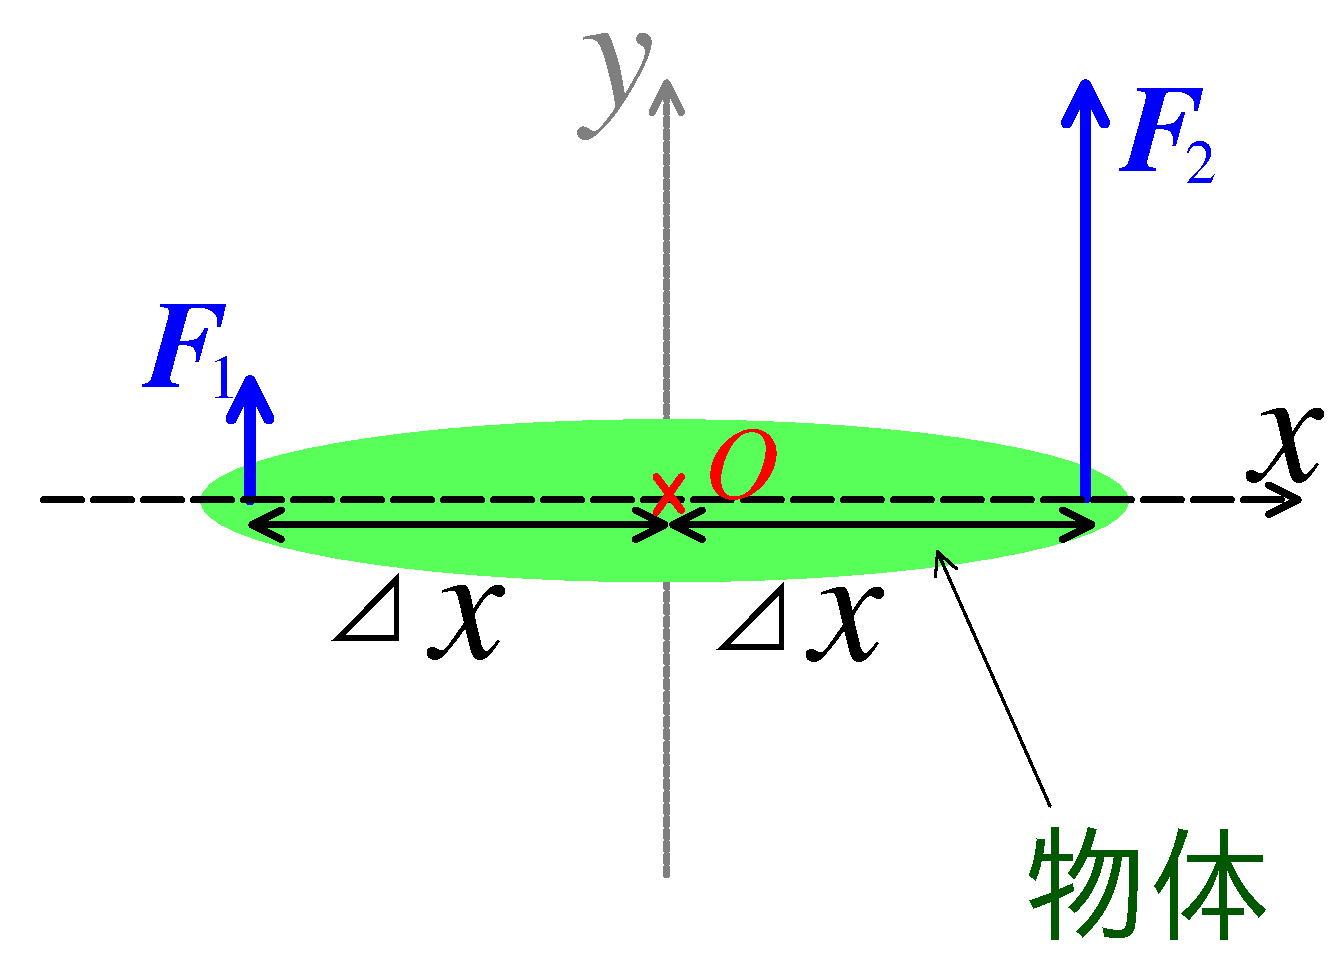
\includegraphics[keepaspectratio, width=4cm,height=2.87cm,clip]{rot_gaiseki1.pdf}
                        \caption{物体(葉)の回転1}
                        \label{fig:rot_gaiseki1}
                    \end{center}
                        \end{minipage}
                    \end{tabular}
                \end{figure}

        葉が原点を中心に回転するには,
        水の流れが原点の中心を境に,
        その勢いが異なっていればよい.
        図\ref{fig:rotrotrot}でいえば,左側の勢いと右側の勢いが
        違っていればよいということである.
        この図はもっと簡単になる.

        この図\ref{fig:rot_gaiseki1}で,左右両方の原点を中心とする力のモーメント
        を考えれば,左側が $F_{1}\Delta x$ であり,右側が $F_{2}\Delta x$ である.
        ここで,図より $F_{1}<F_{2}$ であるから($\Delta x$ は共通であるとする),
        この二つの力のモーメントのは互いに異なった値であり,従って,
        物体は回転をしているはずである
            \footnote{
                回転するように仮定を設けいているので,当たり前と言ってしまえばそうだが,
                確かに回転を表現できるという確認をここでしたのである.
            }.

        ここからが少しヤッカイな部分だが,それは今考えている対象は
        物体の回転ではなく水の回転,つまり“渦”である.
        この渦とはベクトルの回転である.
        物体の回転そのものを
        見るときは力のモーメントを考えればよかったが,
        ベクトルの回転では力のモーメントなんてものは直接には定義できない.
        だから,ベクトル(渦)の上に物体を置いて,その回転でもって
        ベクトルの回転の様子をうかがってみようとしたのである.
        そしてそれによって,ベクトルの回転の様子を,物体の回転として
        観測できることが分かった.この考えをもっと進めていこう.
        簡単のために,原点付近の水の様子を考えてみる.

        力の方向が左右で同じ方向を向いていなくともかまわない.
                \begin{figure}[hbt]
                    \begin{tabular}{cc}
                        \begin{minipage}{0.5\hsize}
                    \begin{center}
                        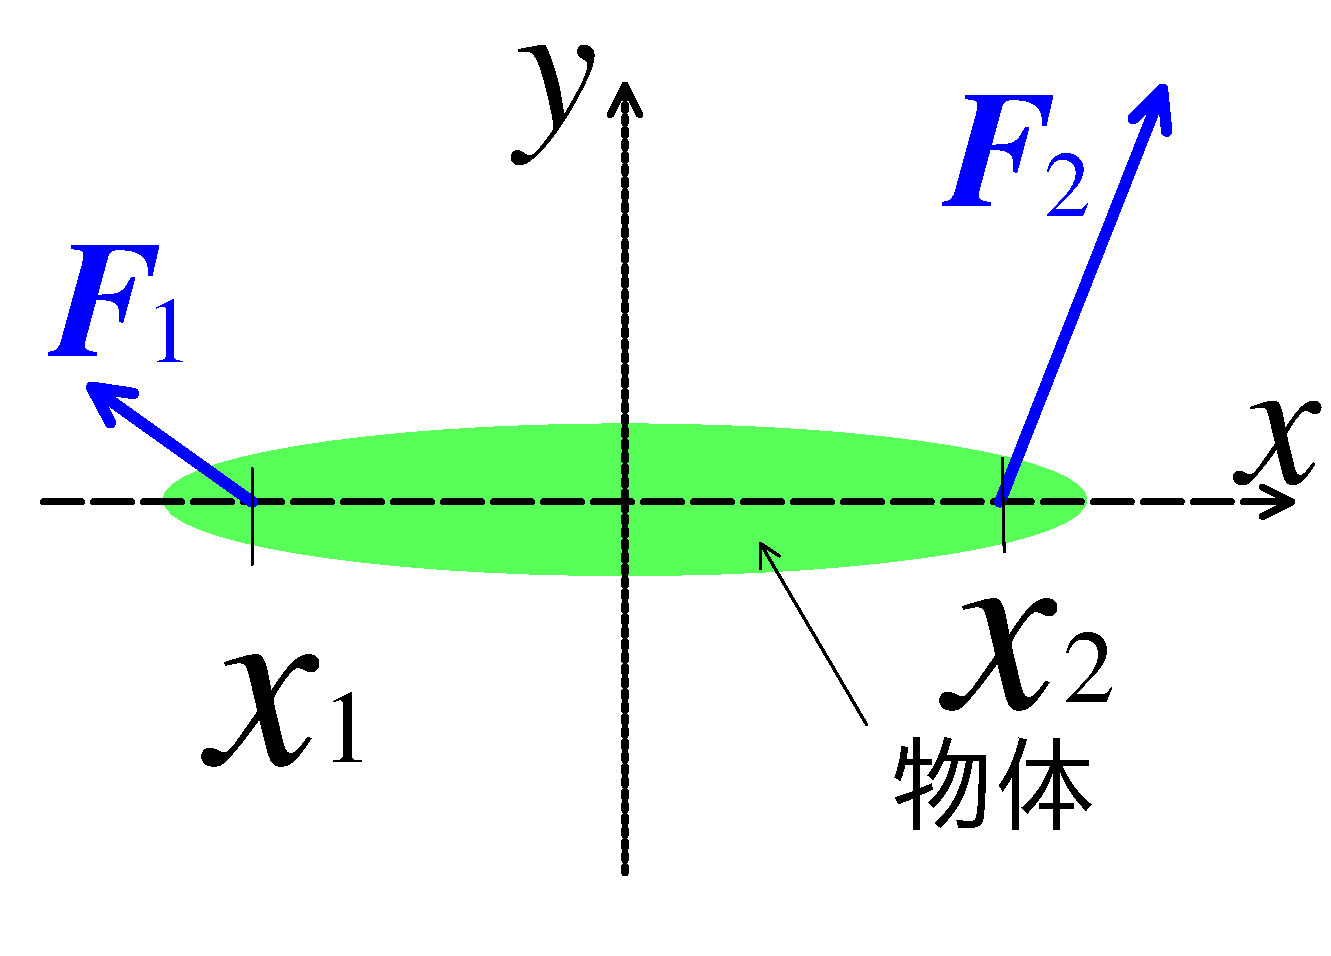
\includegraphics[keepaspectratio, width=4cm,height=2.87cm,clip]{rot_gaiseki2.pdf}
                        \caption{物体(葉)の回転2}
                        \label{fig:rot_gaiseki2}
                    \end{center}
                        \end{minipage}
                        \begin{minipage}{0.5\hsize}
                    \begin{center}
                        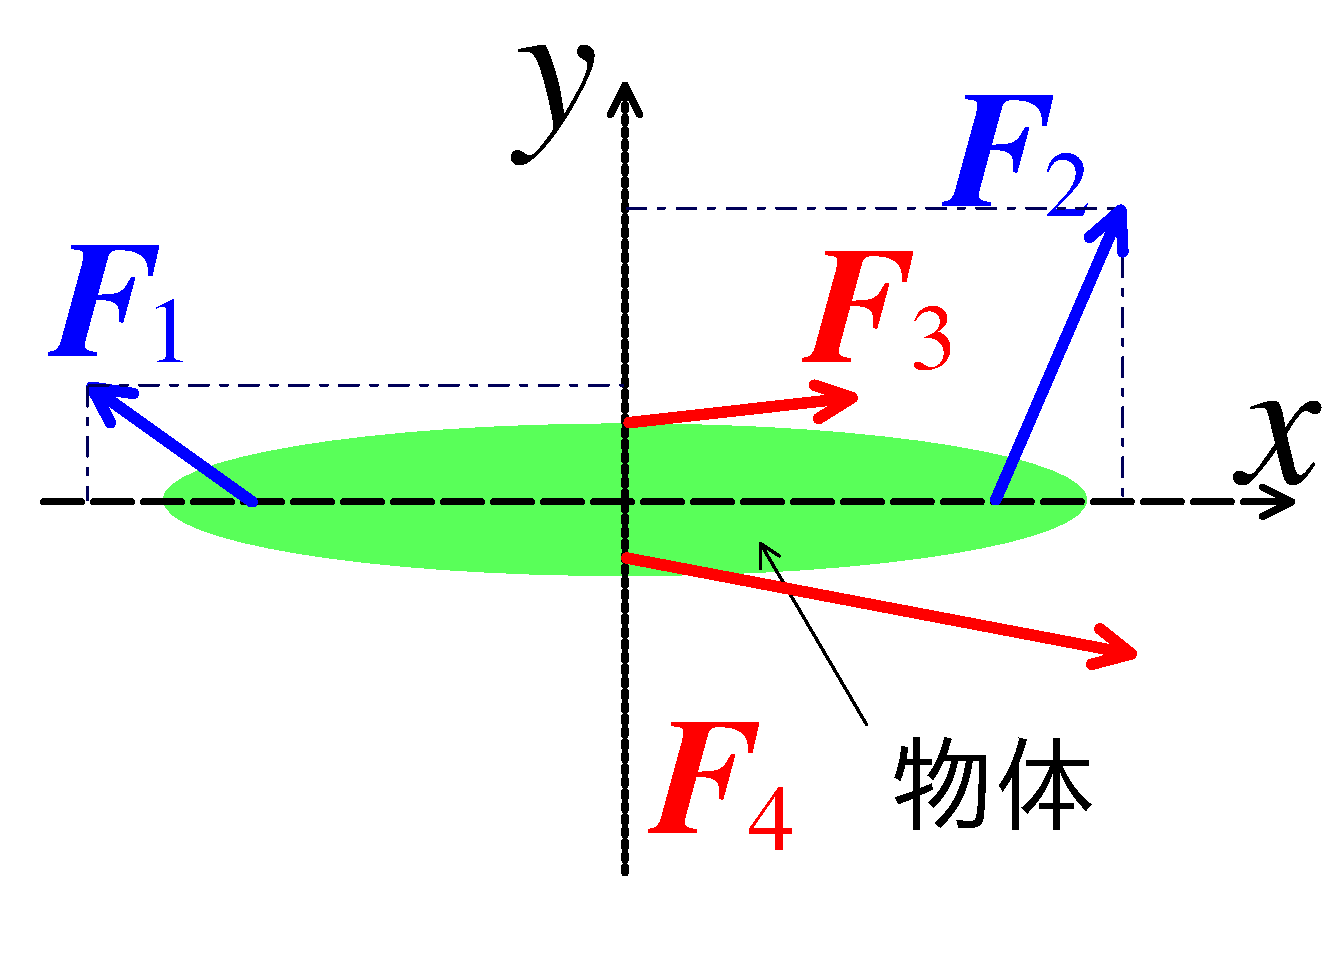
\includegraphics[keepaspectratio, width=4cm,height=2.87cm,clip]{rotation12.pdf}
                        \caption{物体(葉)の回転3}
                        \label{fig:rotation12}
                    \end{center}
                        \end{minipage}
                    \end{tabular}
                \end{figure}

        この図のような状況でベクトルの渦が起こるには,物体にかかる
        $x$ 方向と$y$ 方向の2方向で考えればよい.それを図\ref{fig:rotation12}に示す.

        ベクトル場とはここでは物体が水の流れから受ける力のことだが,
        これを $\bF(\,x,\,y\,)$ とする.
        ここでは話を簡単にするために,ベクトル場は時間に依存しないとした.

        先ほど考えた左右それぞれ力のモーメントの関係は $\bF_{1}\Delta x > \bF_{2}\Delta x$ であった.
        これを以下のように書き直す.
            \begin{align*}
                F_{1}\Delta x - F_{2}\Delta x &>& 0.  \\
                (F_{1} - F_{2})\Delta x &>& 0.
            \end{align*}
        さらにこの式の左辺は0より大きいので,
        何らかの定数,もしくは関数であるので,
        それを $a(\br\,,\,\,t)$ と
        書いて,
            \begin{equation*}
                (\bF_{1} - \bF_{2})\Delta x =a(\br\,,\,\,t)
            \end{equation*}
        とする.今考えている力 $F$ は,$x$ 座標と $y$ 座標ごとに違うはずである.
        つまり,$F$ は $x$ と $y$ の関数であるから,
            \begin{equation*}
                ( F(x_{1} ,\, y_{1}) - F(x_{2} ,\, y_{2}) )\Delta x =a(\br\,,\,\,t).
            \end{equation*}
        今考えているのは,原点付近の水の回転の様子であり,
        $x_{1}$ と $x_{2}$ はさほど離れていないと考えてよい.
        $x_{1}$ と $x_{2}$ の距離は前の図で $2\Delta x$ としていた.
        $2\Delta x$ を $h$ に置き換えてしまおう.
        つまり,$x_{2} = x_{1} + h$ である.
            \begin{equation*}
                ( F(x_{1} ,\, y_{1}) - F(x_{1} + h ,\, y_{2}) )\Delta x =a(\br\,,\,\,t).
            \end{equation*}
        上式の左辺第一項と第二項を入れ替えてみよう.
            \begin{equation*}
                ( F(x_{1} + h ,\, y_{2})  -  F(x_{1} ,\, y_{1})  )\Delta x = -a(\br\,,\,\,t).
            \end{equation*}

        ところで,物体の回転を現すには
        ベクトルの外積を用いた.

        ベクトル $\bA=(A_{x},\, A_{y},\, A_{z})$ の回転 $\drot$ は次式で定義される.
            \begin{align}
                \drot\bA:=
                \left(
                \frac{\rd A_{z}}{\rd y}-\frac{\rd A_{y}}{\rd z}\, ,\,\,
                \frac{\rd A_{x}}{\rd z}-\frac{\rd A_{z}}{\rd x}\, ,\,\,
                \frac{\rd A_{y}}{\rd x}-\frac{\rd A_{x}}{\rd y}
                \right)
            \end{align}

 \subsubsection{ベクトルの勾配($\rm{grad}$)}
        ベクトル $\bA=(A_{x},\, A_{y},\, A_{z})$ の勾配 $\dgrad$ は次式で定義される.
            \begin{align}
                \ddiv\bA:=
                \left(
                \frac{\rd \bA}{\rd x}\, ,\,\,
                \frac{\rd \bA}{\rd y}\, ,\,\,
                \frac{\rd \bA}{\rd z}
                \right)
            \end{align}




 \subsubsection{ベクトル解析の公式(演算子)}
            \begin{align}
                \Delta:=
                \mathrm{div\, grad}=
                \frac{\rd^{2}}{\rd x^{2}}+
                \frac{\rd^{2}}{\rd y^{2}}+
                \frac{\rd^{2}}{\rd z^{2}}
            \end{align}
            \begin{align}
                \mathrm{rot\, rot}
                =\mathrm{grad\, div}-\Delta
            \end{align}



 \subsubsection{ストークスの定理}
        任意の閉曲線を $l$,この閉曲線を縁とする曲面を $S_{l}$ と表す.
        また,閉曲線 $l$ の単位接線ベクトルを $\bt$ と表す.このとき,
        任意の3次元ベクトル $\bA$ に対して,
            \begin{align}
                \int_{S_{l}} (\drot \bA)\cdot\textit{\textbf{n}}\,\df S_{l}
                =\oint_{l} \bA\cdot\bt\,\df l
            \end{align}
        が成り立つ.これを \textbf{ストークスの定理} という.



\chapter{行列}
%   %-----------------------------------------------------------------------------------------------
%   %  Input
%   %    File Name : PhysNote_Math_Matrix.tex
%   %    説明      : 「行列」について.考え方と使い方.
%   %-----------------------------------------------------------------------------------------------
        %===================================================================================================
%  Chapter : 行列
%  説明    : 行列の基本的な計算規則,座標変換について
%===================================================================================================
%   %==========================================================================
%   %  Section
%   %==========================================================================
    \section{行列とは}



%====================================================================================================
%  以降は,付録(Appendix)
%====================================================================================================
    \appendix

%===================================================================================================
%  Part : 思想
%  説明 : 思考の基礎・基本を考える
%===================================================================================================
    \part{思想}
%   %-----------------------------------------------------------------------------------------------
%   %  Input
%   %    File Name : PhysNote_Introduction.tex
%   %    説明      : 「思想」トップファイル
%   %                表現(言語,絵),知覚・直感・思考 等 について,考える
%   %-----------------------------------------------------------------------------------------------
        %===================================================================================================
%  Chapter : 感覚・思想・表現
%  説明    : 物事を考える上での,根本的な思想を記述する
%===================================================================================================
\chapter{感覚$\cdot$思考$\cdot$表現}
    \begin{mycomment}
        この章は,私の個人的な考えをメモしておくものである.だから,記述内容が
        誤っているかもしれず,考え違いや,誤解が含まれていることと思う.
        誰とも議論もせずに記述することであるから,偏った考え方になりがちだし,
        最悪の場合,矛盾がふくまれているだろう.それにもかかわらず,
        この章の文章は"言い切り"の形で記述する.いちいち,「だと思う」という
        語彙を文章末尾につけてしまうと,読みにくくなってしまうし,第一,カッコ悪い.
        なので,偏った考え方や誤った主張を強く強調していると思われるかもしれないが,
        そうではなく,単に現在の私の考えをメモしているものに過ぎないと,捉えてもらいたい.
    \end{mycomment}
%   %==========================================================================
%   %  Section
%   %==========================================================================
        \section{根拠なしに,確信できること}
            根拠なしに確信を持てることは,「考えられる」ということである.
            そして,考えるという行為は,言葉
                \footnote{
                    ここで言う \textbf{言葉} とは,“書くことによる表現”と“話すことによる表現”
                    の両方を指す意味で使っている.
                }
            を用いて行われてることも,根拠なしに
            認めることができる
                \footnote{
                    「言葉なしに考える」という行為は可能だろうか.
                    少なくとも,私には実行不可能である.
                }.

            何かものを考えるときには,考えるための材料と道具が必要である.
            材料というのは経験であり,道具というのは言葉である.
            考えるという行為とは,経験を道具により整理して,その経験に対する
            理解を深めるという行為である.

            私たちの経験する全ての事柄を,\textbf{世界} と表現することにしよう
                \footnote{
                    ここでいう \textbf{世界} とは,世界の国々を表しているのではない.
                    私たちが目や耳などの,いわゆる五感で感じ取る全てのことを総合して,
                    「世界」と表現する.
                }.
            私たちは,世界を経験をできる.経験を記憶できる.
            また,経験を不思議がったり,その不思議を考えられる.
            そして,その考えを言葉や絵で表現できる.そして,このような表現を
            行うことで,自分以外の相手に自分の考えを伝えることができる.

            これが,私の「考えること」の根本的な思想である.これからの物理学の学習は,
            この思想のもとに行う.

            \begin{memo}{言葉と思考の順序}
                考えるという行為は,言葉を使って行われう行為である.もっと強い言い方を
                すると,考えるという行為は言葉なしに行うことは不可能である.つまり,
                言葉を習得する以前は,ものを考えることができないことになる.
                となると,言葉の見習得の赤ん坊は,ものを考えることができないのだろうか.
                この問題に対する,私が納得のできる答えは,まだ存在していない.

                しかし,これだけは言える.言葉の習得する以前から,この世界を感じている.
                世界を感じるという経験の1つに,言葉がある.経験が「思考する」という
                行為の基礎に位置するのである.しかし,この推論に確証はもてない.
                経験が思考の基礎をなすということ
                を,今から身をもって体験することができないからだ.
                言葉習得以前の状態にもどり,言語を習得しなくとも世界を感じとることが
                できるのだな,という感覚を体験できればよいが,これは不可能である.
                推論をいくら重ねたところで,あるいは,多くの言語見習得の赤ん坊を
                観察したところで,自分自身で実感できないので,納得はできない.
                納得はいかないけれど,今の私は言語を扱っている
                    \footnote{
                        少なくとも,とりあえずの不都合なく,意思疎通ができる程度に.
                   }.
                また,その習得に多くの時間を費やしたことも記憶にある.ということは,
                言語見習得の時期があったいう推論は妥当であるとも思える
                    \footnote{
                        実際に言語見習得の時期の記憶がないので,単なる推論でしかない.
                    }.
            \end{memo}

            \begin{memo}{言葉の習得}
                言葉は,人間が生まれながらにしてもっているものではない.
                言葉は,意思疎通を行うために,先人の経験により発明され,
                洗練されてきたものである.

                私たちは,生まれてから自然と母国語の文法を習得する
                    \footnote{
                        国語の時間に,強制的に習得させられることもあるだろう.
                        ひらがなや,カタカナ,漢字を覚えるのには苦労したはず.
                        また,使い慣れない語彙を使用し始める場合,単語そのものを
                        誤って使ってしまい(「つくる」を「くつる」に間違うなど),
                        大人から,その場で間違いを指摘され,修正された経験もあったことだろう.
                        しかし,その間違いの指摘は言葉によって行われたのであり,
                        それにより,誤りを自覚してそれを修正しようと努力できたはずである,
                        全ての言葉を自然に習得できるわけではないのだが,言葉の基本的な使い方
                        は誰から教わったものではなく,自分の周囲に飛び交っていた母国語を
                        聞くことにより,非言語的に習得するのである(
                        そうでなければ,言葉の使い方を間違っときの,その間違いの指摘を
                        理解することができないことになる).
                        言葉の文法を,0から
                        言葉により説明することはできない.というのも,文法を説明しようとすると,
                        その説明自体に言葉を使用せざるを得ず,
                        つまり,「文法を知る前に文法を知っていなければならない」といった,
                        自己言及的な矛盾がおこるからである.しかし,現に私たちは母国語の文法を
                        習得して使用している.
                    }.
                母国語は体系的に教わることない.常に生の言葉を聞き,そして,その時の状況を
                機能するすべての感覚器から感じ取り,言葉の使用法を身につける.論理学や数学
                で言うところの公理
                    \footnote{
                        最も基礎となる,疑いようのない事実のこと.万人が根拠なしに正しいと
                        感じること.例えば,数学で言うと,「A$=$B で B$=$C のとき,A$=$C」
                        といった感じの,最も基本的なお約束のことを言う.これは有無を言わさず
                        たたきつけられることである.その根拠を求めてはならない.公理の根拠
                        なんてものは,はじめから存在しないのだから.言い方を変えれば,何かを
                        論理的に考えようとした時に,その根拠が求められることがあるが,
                        その根拠は果てしなく問うことは不可能である.いずれは,根拠を示すことができない
                        当たり前すぎる事柄に,直面することだろう.それを公理というのである.
                    }
                があるわけでもなく,ただ漠然と,その使われ方を悟り,自分のものとしていく.
                人間には,言葉を習得する能力が生まれながらにして備わっているのだ.
                なぜだろうか.意思疎通をうまい具合に行うためだとか,いろいろ後付的な
                説明がなされることもあろうが,そんなことは確かめようがない.なんとでも言えるのだ.
                ここでは,深く考えずに,「私は言葉を使うことができる」ということを,
                素直にそのままの形で受け入れておこう.
            \end{memo}

            \begin{memo}{意思疎通}
                言葉はどんな時に使われるのだろうか.いや,おかしな疑問を投げかけてしまった.
                そんなの,意思疎通を行うために決まっているじゃないか.本当に,そうなのか.
                言葉でだけで,意思疎通が十分に可能だろうか.いや,できないはずだ.
                誤解や言い間違いなどで,正しく意思疎通ができないこともあるだろう.
                言葉だけで十分に意思疎通はできないのは,当たり前で,そのために,他の手段として,
                手や体を動かして(身振り手振り)表現することもある
                    \footnote{
                        別れ際に相手に対して手を振ったり,違うことを示すために首を横に振ったりするだろう.
                    }.
                図を使って表現することもあろう.音楽で気分を表現したりもするだろう
                    \footnote{
                        気分が良い時には,鼻歌が自然にでたり,踊ることだってするでしょ?
                    }.
                とにかく,意思疎通のための道具は,言葉だけではない.

                だけど,ここまで書いといてなんだけども,ノートで自分の考えを示すのには,
                図と言葉でしか表現できない.なんともやりづらいが,どうしようもない.
                ここは我慢して,図と言葉だけで伝わるように,記述しなければならない.
                図と言葉だけで,どれだけのことが表現できるかわからないが,頑張って考えながら,
                記述していこう.たとえ時間がかかろうとも,文が長ったらしくなろうとも,
                丁寧に記述していけば,どんなことでも言葉で伝えることができると信じて,
                記述していこう.

                私は考えることができ,それを言葉で表現でき,そして,
                その言葉によって他者に自分の考えを伝える事ができると信じる.
                そして,逆に,他人の表現する言葉を理解し,他者の考えを受け入れられることも,信じる.
                さらに,自分と他人とで会話を続けることにより,より深く正確に互いの考えを
                理解し合えると信じよう.ここのところをこれ以上疑いだすと,言語哲学的な世界に
                陥ることになり,抜け出せなくなってしまう.もうこれ以上,言葉について考える
                事はせずに,話を先に進めよう.
            \end{memo}

%   %==========================================================================
%   %  Section
%   %==========================================================================
        \section{表現}
            思考を表現する最も有効な道具が,言葉である.また,時には,言葉よりも絵に書いたほうが
            より伝わりやすいこともあろう
                \footnote{
                    宣伝看板や,ポスターなどが良い例だ.
                }.
            言葉や絵以外にも,ある規則に従った記号により,思考を
            表現することも可能である.
                \footnote{
                    特に,音楽は言葉によって表すことは難しい.原理的に不可能とは言わないが,
                    そうして表現できたものは,とても煩雑で理解しがたい表現になっていることだろう.
                    では,音楽を伝える方法はないのかというと,もちろん,そんなことはない.
                    周知の通り,\textbf{楽譜} という音楽独特の表現方法が考えだされている.
                    楽譜は絵でも言葉でもないが,人間のもっている,ある種の感覚を表現するものである.

                    また,他例を上げれば,数学や記号論理学なども,記号の羅列である.

                    「言葉」という語彙は,これらの例のような意味を含めて使われることも多い.
                    これは,文脈によって理解できるだろう(著者はそうわかるように書くべきだ).
                }.
            表現するという行為は,言うまでもなく,
            自分の考えや思いを自分以外の相手に伝えるということである.

%   %==========================================================================
%   %  Section
%   %==========================================================================
        \section{「科学」の思想}
            "科学的" という言葉は日常的に使用される.特に,最新技術という意味で
            使用されることが多いように感じる.しかし,"科学的" とはどういうことかを
            考えてみると,残念なことに,明確なイメージを描けないことに気付く.

            \begin{figure}[hbt]
                \begin{center}
                    \includegraphicslarge{SekaiKansokuBunrui01.pdf}
                    \caption{科学的に扱えることの範囲}
                    \label{fig:ThomomExpElec001}
                \end{center}
            \end{figure}

        \begin{memo}{基礎がない,考えが循環する}
            ものごとを考える前には,経験が必要である.考えは,その経験の不思議さ
            を基に行われるからである.では,この経験はどう捉えら得るのだろうか.
            当然ながら,経験は眼や耳などの五感で捉えられる.そして,その認識は,
            脳に伝わって初めて経験を実感し,記憶される.だから,最も基礎的な
            学問分野は脳科学なのだろうか.いや,これは違う.脳は生物の一部であり,
            脳科学は生物学の一分野として位置するものである.生物はその組織の
            内部で,化学反応を起こして生命を維持している.従って,化学が,生物学よりも
            基礎的な位置にあるはずである.また,化学で扱われる化学反応は,突き詰めれば,
            原子や分子の結びつきであり,原子や分子の運動は物理学により説明される.
            そして,物理学は数理的推論をその拠り所としていて,数学と論理学が物理学
            の基礎となっている.数学と論理学は,元を正せば,私達が日常生活の中で使用している
            言語の曖昧な部分を除き,正しい思考とは何かを探る学問である.そして,その思考を
            行うには,前もってその思考に関する経験が必要である.経験は五感で感じ,脳によって
            認識され,$\cdots$.

            循環する.上記のどこかに誤りがあるのだろうか.
        \end{memo}

%===================================================================================================
%  Chapter :
%  説明    :
%===================================================================================================
\chapter{論理}


%===================================================================================================
%  Part : 思うこと,思ったこと
%  説明 : 自分なりの考え方・思想についての記述を行う.
%===================================================================================================
    \part{思うこと,思ったこと}
%   %-----------------------------------------------------------------------------------------------
%   %  Input
%   %    File Name : PhysNote_Omoukoto.tex
%   %    説明      : 物理学を考える以前の,基本思想を記述する.
%   %-----------------------------------------------------------------------------------------------
        \normalsize
%%**************************************************************************************************
%%
%% File Name : PhysNote_MessageFirst.tex
%% 説明      : 物理学の導入をかねた,古典力学(ニュートン力学と解析力学)を学習する.
%%
%%**************************************************************************************************

%===================================================================================================
%  Chapter : 素朴な疑問
%  説明    : 「考えるとはどういうことか」とかを考えてみる.
%===================================================================================================
    \chapter{素朴な疑問}
%   %-----------------------------------------------------------------------------------------------
%   %  Input
%   %    File Name : PhysNote_Math_MsgFirst.tex
%   %    説明      : 考えるって何だろう.
%   %-----------------------------------------------------------------------------------------------
        %===================================================================================================
%  Chapter : はじめに
%  説明    : 「考えるとはどういうことか」とかを考えてみる.
%===================================================================================================
%   %==========================================================================
%   %  Section
%   %==========================================================================
        \section{最も基本的なこと}
            学問を学ぶにあたって,“最も基本的で信頼できること”を
            基礎にして,その上で学習を進めることは,当たり前のこと
            である.では,その“最も基本的で信頼できること”とは何
            だろうか.

            これは多分に哲学的な問題提起であるが,ここでは,今後,
            物理学の学習を進めていくにあたり,思想の最も基本的なよ
            りどころを確認するためのもので,哲学に深く介入すること
            はしない
                \footnote{
                    正直に書こう.哲学に介入することは,私のような
                    低レベルの頭では,不可能である.開き直って,言
                    うならば,そこまで深く考えてもしょうがない,思
                    うところもある.
                }.

            私は,最も基本的で信頼できることとして,「考えること」
            をあげたい.これは独我論てきな思想である.独我論とは,
            極端に言えば,この世界に存在を確信できるのは私の思考の
            みであり,私が今感じている温度や光などは,私の思考によ
            って感じていると錯覚しているのであって,実在しているの
            ではない,という考え方である.こう考えると,自分以外の
            人間とは,私の思考が作り出した幻想であり,実際にそこに
            いるわけではないということになる.そう,信じられるのは,
            今考えている私がここにあるということである.


%   %==========================================================================
%   %  Section
%   %==========================================================================
        \section{私の思想の根本}
            では,もう一段階突っ込んでみよう.「考える」ということ
            とは,どうすることなのだろうか.「考える」という動詞の
            使い方は,おおよそ次の様だろう.
                今晩の献立を考える.
                人の気持ちを考える.
                将来の進路を考える…
            などなど.
            考えるという作業を行っているとき,「言葉」を道具として
            使う.また,時には「図」を使って考えることもあるだろう
            が,これは単に言葉で考えるよりも図を用いた方が考えやす
            いからであり,言葉では思考不可能であるということではな
            い.思考はすべて言葉で表現できる(と信じる).

            私の,最も信頼できる唯一の基本的なことである,私の思考
            は言葉を用いて実行される.では,その次の疑問として,
            「言葉」とは何か,ということが生まれてこよう.

            この章では,「考えるとは何か」について,私が考えること,
            というか,思っていることを記述する.


%   %==========================================================================
%   %  Section
%   %==========================================================================
        \section{思考の道具}
            考えるという動作は,言葉を用いて行っていることを確認し
            た.言葉を用いて考えているので,この言葉の使用限界が思
            考の限界であるということになる
                \footnote{
                    Wittgensteinは「論理哲学論考」という著
                    作で,このことを詳しく論じている.後に,彼自身
                    によってこの著作は間違いであるとされてしまうの
                    であるが…このノートでは,そこまで深く入ら
                    ない.だって,とっても難しいから.
                }.

            単に「言葉」といっても,それは様々な形で存在する.英語
            やドイツ語,フランス語,イタリア語などたくさんだ.各国
            の人々は,自国のあるいは使い慣れた言葉で考えていること
            だろう.ここでは,どのような国の言葉も,その適用限界
            は変わらないと仮定して,話を進めて生きたい.多少,言葉
            の適用限界があったとしても,それは話にならないくらい,
            細かいことに過ぎないと信じる
                \footnote{
                    実際,各国の人々が同じように「考えて」いるとい
                    う現状からこのような仮定を設けてもよいと考えて
                    いる.ただし,ここでは,「考える」ということに
                    関して,文化や伝統,生活習慣などの影響は無視す
                    る.
                }.

             もちろん,言葉で説明できないこともある.ある種の“ひらめき”
             とか,もろもろの感情とかを言葉で表現することは難しいこ
             とである.いや,不可能といってもよい.しかし,考えると
             いうことに関しては,言葉のもつ機能は十分である考える.私
             は,「どんな思考も言葉にできる」と信じて,こ
             のノートを作成する.


%   %==========================================================================
%   %  Section
%   %==========================================================================
        \section{言語の曖昧さ}
            思考を言葉で記述できたとしよう.その次に問題となるのは,どれ
            だけ正確に思考できるか,ということだろう.いや,視点を変えて
            言い換えよう.私たちが行う多くの思考の中で,正しい思考とはど
            ういうものなのかを,整理しなければいけない.わけのわからない
            思考や,意味を成さない思考などを排除したいのである.


%   %==========================================================================
%   %  Section
%   %==========================================================================
        \section{日常言語}
            普段の生活で使っている言語は,曖昧な表現をすることが多い.曖昧
            表現というのは,人によって解釈が異なってしまう表現のことである.
            「美しい景色」だの,「大きな木」だのと言って,すべての人が同じ
            情景を浮かべることはまずない.これでは正しい思考が,十分ではな
            い他の人間に伝わることはない.

            しかし,このような例から,普段使っている言語は正しい思考に適し
            ていないと,判断してはいけない.事実,過去の多くの頭のいい学者
            さん達は,言語を用いて正しい思考をし,様々な学問を作り上げてい
            る.大切なのは,曖昧な表現を避けることである.ただ,言語には使
            い方によって,曖昧に表現できてしまうだけなのである.

            では,言語の曖昧な表現を使わないようにするには,どうしたらよい
            だろうか.まず考えつくのは,日常言語から万人が認める最も基本的
            な部分を抽出し,それを元に思考をすればよいことである.言語の最
            も基本的な部分とは,「論理」である.次に,論理について簡単に触
            れよう.




%===================================================================================================
%  Chapter : 論理学とか,数学とか
%  説明    : 物理学より,思考方法としてより基礎的なことである,論理・数学について考えてみる.
%===================================================================================================
    \chapter{論理学とか,数学とか}
%   %-----------------------------------------------------------------------------------------------
%   %  Input
%   %    File Name : PhysNote_CM_LogicMathEtc.tex
%   %    説明      : 数学とか論理学について,物理学のもっと基礎にある学問についての断片的な学習メモ.
%   %-----------------------------------------------------------------------------------------------
        %===================================================================================================
%  Chapter : 論理学とか,数学とか
%  説明    : 物理学より,思考方法としてより基礎的なことである,論理・数学について考えてみる.
%===================================================================================================

%   %==========================================================================
%   %  Section
%   %==========================================================================
        \section{論理}
            私たちが普段の生活で使っている言語のうち,曖昧な使い方を避けて
            ,万人に共通に伝わるようにしたい.そのためには,\textbf{論理}
            と言うものを考える必要がある.論理は,日常言語の中の一部にある
            .相手に自分の考えを伝えるとき,物事を筋道立てて伝えようとする
            だろう.自分の考えをできるだけ性格に相手に知ってほしいからであ
            る.さて,このとき私たちは,論理を使っているのである.論理は,
            何個かの公理
                \footnote{
                    公理:万人が認める事実のこと.何の反論なしに認めなけれ
                    ばならないことである.ある仮説を検証するとき,その仮説
                    の根拠をどんどん探ることになる --- AはBとCからなってい
                    て,BはDから,CはEを基にしている・・・と言うように---.
                    しかし,いつまでもこれが続くわけではない.いつかは,ど
                    うしようもなく“当たり前すぎて”,説明ができないことに
                    たどり着く.公理とは,その当たり前の事実を明示するもの
                    である.
                }
            と推論規則
                \footnote{
                    推論規則:ある仮定から,別の仮説を作り出せる規則のこと
                    .公理と同様,有無を言わさず認めさせられるものである.
                }
            を基に構成される.少数の公理と推論規則から,主張したいことがす
            べて主張できる体系を作ることが学問の目的である.これを思考経済
            と言ったりする.公理と推論規則は,少なければ少ないほどよい.



%   %==========================================================================
%   %  Section
%   %==========================================================================
        \section{論理学}
            この論理について,詳しく研究する学問に \textbf{論理学} がある
            .ある仮説を記述した文で,本当か嘘かをはっきりと区別できる文の
            ことを,\textbf{命題} という.論理学はいくつかの必要最小限の公
            理と推論規則を組み合わせ,命題の証明を繰り返し発展させていくも
            のである.命題と推論規則の組み合わせのことを,\textbf{公理系} と
            言う.この公理系には,次の3つの性質が備わっている必要がある.一
            つは \textbf{独立性} で,公理形の中のどの1つの公理を選んでも,
            他の公理からその公理を証明できないような性質である.
            二つ目は \textbf{完全性} と言われるもので,主張したい命題が,そ
            の公理系からすべて導けることである.三つ目は \textbf{無矛盾性} と
            言われるもので,公理系に互いに矛盾する公理を含んでいないことで
            ある.

            論理学とは考察の足固めである公理系を設計し,体系を作り上げて
            いく学問でもあるのだ.どれだけ詳しく説明できるかと言う疑問の最
            も根本的な部分の研究がここでなされる.



%   %==========================================================================
%   %  Section
%   %==========================================================================
        \section{数学}
            数学とは,論理に複素数を組み合わせた学問であると言える.その研究
            の対象はおもに,複素数である.複素数の一部には,自然数が含まれて
            いる.残念なことに,自然数を含む公理系には,完全性,無矛盾性が常
            に保たれていると言う保障がないことが知られている.この事実は
            G\"{o}delの \textbf{不完全性定理} とよばれている
                \footnote{
                    参考文献:廣瀬 健,横田 一正 [著],「ゲーデルの世界」,
                    鳴海社,2004
                }.

            集合論により無限を扱えるようになってきたころ,この無限を起因とし
            て様々なパラドクスが発見されることとなった.「自分自身を要素とし
            て含まないすべての集合」がその最も有名なものである.ちょっと考え
            てみよう.
                \begin{equation*}
                    \omega:\;\;\mbox{自分自身を要素として含まないすべての集合}
                \end{equation*}
            と定義しよう.そして,次の問題,すなわち
                \begin{equation*}
                    \mbox{問題}:\;\;\omega \mbox{自身は,} \omega \mbox{に含まれるか否か}
                \end{equation*}
            を考えてみよう.すぐに明らかな矛盾が見えてくるだろう.

            $\omega$ は自分自身に含まれると仮定してみる.すると,$\omega$ の
            定義「自分自身を要素として含まない」という仮定に矛盾する.では,
            $\omega$ は自分自身に含まれないと仮定したらどうか.実はこれでも
            矛盾が生じる.なぜなら,「自分自身要素としてを含まない」という
            定義上,仮定で「自分自身は含まない」言っているので,自分自身を
            含むべきだと言う結論が出てしまう.肯定的に仮定しようが,否
            定的に仮定しようが,どちらにしても結果はその仮定と矛盾するので
            ある.

            Russellらは,この問題を解決しようと階という概念を導入し,命題
            に自分自身を含むことのないように制限を加えた.しかし,問題はこれ
            だけではとどまらず,山のように残されていた.

            Hilbertはこのような問題の山を,数学の危機であると自覚し,これを
            解決しようと計画した.Hilbertはこの数学の危機と言われる問題を23
            個の命題にまとめた.そして彼は,この23の問題を証明し解決しようと
            呼びかけた.G\"{o}delの不完全性定理はこの23の問題のうちの一つ
                \footnote{
                    第2番目に掲げられていた問題だった.
                }
            の否定的な回答であった.

            だから,物理学に公理系を作成して,論理的に構成しようとしても,無駄
            である.しかし,物理学は自然の構成を探る学問だから,この点に関して
            はあまり気にすることはないと思う.


%   %==========================================================================
%   %  Section
%   %==========================================================================
        \section{物理学}
            物理学は,自然がどのようになっているかを探る学問である.
                \footnote{
                    "なぜ"自然が私たちの感じているようになっているのかを探る学
                    問では\textbf{ない}.
                }
            「なぜ(Why)」を問うのではなく,「どのように(How)」を問うのであ
            る.

            なぜ自然がこのように
                \footnote{
                    普段の生活で,私たちが感じている自然を思い浮かべてみて.
                }
            なっているのか,とか,なぜ宇宙があるのかとかを考えるのは哲学であって,
            物理学ではない.物理学ではこういう,"なぜ"を問うような疑問には答えられない
                \footnote{
                    ただ,"なぜ"という問を深めていく事は可能で,実際に,物理学の発展は
                    その繰り返しである.その様子は.これからの学習で実際に感じることになる.
                }.

            物理学とは,自然の性質を見つけるものである.この「性質」という言葉は
            物理学では \textbf{法則} と呼ばれている
                \footnote{
                    \textbf{法則}:後で詳しく記述する.
                }.
            自然の法則を,実験や数式を通して見つけ出すことが物理学の目的なのだ.

            自然はデタラメに変化しているのではなく,何か一定の法則に従ってい
            るということは,経験上理解できることと思う.例えば,特別に力を加え
            ない限り,高いところから低いところへ,物体は落ちていく.落とした消し
            ゴムは,拾わないと手元に戻ってこないのである.何でだろうか.この原因
            を探り,「法則」として記述するのである.

            このことについては,物理学を学び始めた段階ではまだ実感がわかないかも
            知れない.学習していく過程で,だんだんとわかることだろう.

            このノートでは物理学を学習することが目的である.自然はどのような法則
            に従って変化しているのだろうか.少しずつ考えることにしよう.




%===================================================================================================
%  Chapter : 他愛のない,思ったこと
%  説明    : 他愛のない,思ったことをメモしおこう.
%===================================================================================================
    \chapter{他愛のない,思ったこと}
%   %-----------------------------------------------------------------------------------------------
%   %  Input
%   %    File Name : PhysNote_Apdx_Omoukoto_TaaiNaiOmoukoto.tex
%   %    説明      : 
%   %-----------------------------------------------------------------------------------------------
        %===================================================================================================
%  Chapter : 他愛のない,思ったこと
%  説明    : 
%===================================================================================================

%   %==========================================================================
%   %  Section
%   %==========================================================================
        \section{生まれ変わる?}
            「生まれ変われるとしたら,次は何になっていたい?」と聞かれることが
            ある.この質問には,何も考えずに答えることが,コミュニケーションを
            円滑にする為に良いのだが,やはり引っかかる部分がある.

            引っかかることとは,「生まれ変わる」ということの定義である.生まれ
            変われるか否かということも当然疑問なのだが,それよりももっと疑問な
            ことがある.生まれ変われることが可能かどうかという疑問には,おそら
            く答えることは不可能だろう.生まれ変わることが不可能であるとした
            ら,話はそれで終わりであるので,ここでは,生まれ変われることができ
            るものとして,話を進めたいと思う.

            疑問というのは,“今の記憶が忘れ去られていたとしても,生まれ変わったと言えるか”と
            いうものである.以前までの記憶がない以上,当然,自分自身には生まれ変わ
            ったという意識は生まれない.第三者的な立場にたって,他人の生まれ変
            わる瞬間を見たとしよう.その場合,生まれ変わることが可能だと,納得
            することだろう.しかし,その他人には以前までの記憶がなく,やはり,
            その人にとって,生まれ変わったという意識はないはずである.たとえ,その瞬間を見てい
            たと教えてやったとしても,その人は生まれ変わったのだと明確に認識することは不可能である.

            生まれ変わって以前までの記憶がない以上,たとえ本当に生まれ変わったのだとしても,
            自分自身にとっては,別人であると意識せざるを得ないと考えるのが,自然なのではなかろうか.
            実際,今の私には,こう考えることが一番妥当だと思っている.
            たとえ,生まれれ変わっていたとしても,記憶が残っていない以上,
            それはその人にとって別ものなのだと考えたい.

            まとめよう.求める答えは,生まれ変われるか否か,ということだったが,これには,
            答えることはできない.
            生まれ変わることができないのであれば,話はここで終了になる.もし,
            生まれ変われることがわかったとしても(他人が生まれ変わったことを見るなどして),
            自分自身では認識できないのであれば,それは生まれ変わったと考えるべきではない,
            と思う.

%   %==========================================================================
%   %  Section
%   %==========================================================================
        \section{教科書に書かれていること}
            物理学や化学$\cdot$生物学$\cdot$天文学などの自然現象を説明すべく,それを
            文字として記述し,本という形で記録できる.
            世の中には多くの専門書,教科書,解説書がある.しかし,
            どれをとっても自然現象をすべて説明するものはない.
            つまり,本を読んだところで,世界を理解できるわけではない.
            本を読んでわかることは,先人たちが苦心して築きあげてきた
            壮大な理論体系ではあるものの,自然現象についてのほんの僅かな
            ことでしかない.

            物理学を学ぶということは,物理学の論文や専門書,教科書を
            読むということではなく,実際の自然現象に触れるということ
            である.そして,なぜだろうと疑問に感じることであり,
            さらに,それを解き明かしたいと思うことである.

            物理学を学びたいから物理学の教科書を読む,なんてことは,
            甚だ見当違いである.物理学は自然現象を説明する理論であり,
            つまり,実際に起こっている現象を説明しようとするものである.
            重要なのは,現象に触れること.そして,その現象について,
            その特徴をできるかぎり詳しくしらべること.そうしてやっと,
            現象の特徴はどのような法則に従っているかといった,理論的
            研究に入るのである.

            物理学の本を読むということは,今知られている理論を把握
            するということであり,物理を追求するという行為ではない.
            あくまでも,先人の得た知恵を吸収するということである.
            しかし,それは,探求の第一歩ではない.
            物理学の本を読んで,物理をわかった気になっているとしたら,
            とても残念なことである.


%   %==========================================================================
%   %  Section
%   %==========================================================================
        \section{心配レベル}
            心配という心情には,4つの段階があると思う.それは,次の通りだ.
                \begin{enumerate}
                    \item 心配
                    \item 不安
                    \item 恐怖
                    \item 絶望
                \end{enumerate}
            下に行くほど(数字が大きくなるほど),心配レベルが上がる.
            
            具体例を示してみよう.
            いつもそばにいる大切な人が,一週間の間,自分の前からはなれることに
            なることを考えてみる.海外旅行にでも出かけることにでもしておこう.
            
            その時,あなたは大切な人が,目の前から離れることで,心配になる(はずだ).
            交通事故に遭わないだろうか,悪い人に騙されたりしないだろうか,等々.
            これが,心配という心情だ.この段階では,心配するだけで,何も行動を
            起こさないことだろう.

            一週間たっても,1日,2日,大切な人が帰って来なかったとしよう.
            あなたは不安に陥ることだろう.何があったのか気になって仕方がない.
            こうなると,あなたは,どうにかして,連絡を取ろうと必死になるはずである.
            これが不安という心情.

            どうしても連絡がつかなかったら,その不安は恐怖になる.
            事件に巻き込まれたとか,事故にあったのではないかとかと,考え始める.
            この時,大切な人が傷ついているかもしれないという,恐怖を覚える.

            その恐怖が,最悪の形で現実出会ったとしよう.このとき,あなたは為す術がなく,
            絶望に至る.その後,自分のできる限りの行動を,世の中に対して必死に働きかける
            ことになる.



%   %==========================================================================
%   %  Section
%   %==========================================================================
        \section{"分からないこと" と "知らないこと"}
            突然,新しい環境に放り込まれたとしよう.
            このとき,大変幸福なことに,近くにその環境に詳しい人がいるとする.しかし,
            その人は,私に対して,その環境のことを説明することを
            あまりしない.そのひとは,
            「わからないことがあったら,何でも質問してください」と言う.
            新参者の私にとっては,その環境に詳しい人は,唯一頼りにできる
            大変ありがたい存在である.
            しかし,私がその人に質問するには,時間がかかる.
            自分が分からないことを把握しなければならないからである.
            わからないことを把握するには,知らないことをリストアップしていく
            必要がある.知らないことは,当然,質問できないからだ.例えば,
            「不確定性原理」という言葉を知らない人は,それについて詳しい人が
            そばに居たとしても,質問することはない.
            質問できないのである.

            何が言いたいかというと,教わる側の人間にが取るべき行動は,
            その周囲の環境を,できる限り,見て聞いて把握することである.
            そして,教える側の人間が取るべき行動は,その新参者が知らないことを
            示してあげる事である.

            わからないことが質問できないと言って,嘆く必要はない.
            そんな場合は,周囲の環境を執拗に見たり聞いたりして,
            できる限り早く把握する,という目標があるのだから,
            それを行えば良い.それができなければ,諦めて,
            別の場所に行くより他はない.


%   %-----------------------------------------------------------------------------------------------
%   %  Input
%   %    File Name : PhysNote_Apdx_Vocabularry.tex
%   %    説明      : 故事成語/四字熟語/哲学/思想
%   %-----------------------------------------------------------------------------------------------
        %===================================================================================================
%  Chapter : 語彙メモ
%  説明    : 本や辞典などで知った語彙をノートする
%===================================================================================================

%   %==========================================================================
%   %  Section
%   %==========================================================================
        \section{故事成語}
            \subsection{\ruby{華胥}{かしょ}の\ruby{国}{くに}}
            理想的な世の中のこと.また,心地よい夢の正解のこと.列子から.
                
            \subsection{\ruby{胡蝶}{こちょう}の\ruby{夢}{ゆめ}}
            夢と現実の違いは,実ははっきりとしないということ.また,人生のはかないことのたとえ.荘子から.
                
            \subsection{\ruby{上善}{じょうぜん}は\ruby{水}{みず}のごとし}
            最高の善を,水の性質にたとえたことば.老子から.

            \subsection{\ruby{驥足}{きそく}を\ruby{伸}{の}ばす}
            優秀な才能を存分に発揮することのたとえ.また,自由気ままに行動すること.三国志・蜀書-龐統伝から.

            \subsection{\ruby{驥尾}{きび}に\ruby{付}{ふ}す}
            それほど才能がない者でも,才能があるものについて行けば,何かをやりとげることができることのたとえ.史記-伯夷伝から.

            \subsection{\ruby{木}{き}に\ruby{縁}{よ}りて\ruby{魚}{さかな}を\ruby{求}{もと}む}
            やり方をまちがえると,何も得られないことのたとえ.的外れで,愚かな行為のたとえ.孟子から.

            \subsection{\ruby{人間}{じんかん}\ruby{到}{いた}る\ruby{所}{ところ}に\ruby{青山}{せいざん}\ruby{有}{あ}り}
            骨を埋めるところはどこにでもある.大望を実現するためには,故郷にこだわらず,広い世間に出て活動すべきである,ということ.

            \subsection{\ruby{過}{す}ぎたるは\ruby{及}{およ}ばざるがごとし}
            度が過ぎたものは,足りないものと同様によくない.ものごとには程よさが大切ということ.やりすぎはよくない.足りないのもよくない.ちょうどよいのがいい.論語から.

        \section{メモ}
        \subsection{世界平和評議会(1949年--)}
        世界平和評議会(World Peace Council)は、ポーランド(ワルシャワ)で設立された組織。
        冷戦当時に東側諸国(社会主義国)政府の主導で設立された。日本からは日本共産党系の日本平和委員会が加入している。
        
        \subsection{平和擁護世界大会(1950年)}
        1949年4月,パリで平和擁護世界大会(World Congress of Partisans of Peace)の第1回大会が開かれた.
        冷戦が激化し始める中,フランス政府が東側諸国代表の入国を拒否したため,東側諸国の1国であるチェコスロバキアのプラハでも同時開催された.
        
        1950年’11月16日-22日),ポーランド(ワルシャワで)第2回平和擁護世界大会が開かれた.81か国からの参加者があった(2065人).
        冷戦下において,西側諸国
        \footnote{西側諸国:アメリカ/日本/西ドイツなど}
        と対峙するの東側諸国
        \footnote{東側諸国:ソビエト連邦/ポーランド/東ドイツなど}
        の強い影響を受ける団体であることから,日本と西ドイツの再軍備を非難された.
        一方で,東ドイツやポーランドの再軍備については触れられていなかった.
        また,「世界平和評議会」の設置を決定し,核兵器使用禁止を求める「ストックホルム・アピール」を宣言し,その後5億の署名を集めた.

        \subsection{ストックホルムアピール(1950年)}
        平和擁護世界大会で核兵器の禁止が求められた.さらに核兵器を使用した者を戦争犯罪人とみなすと表明した.
        5億人の賛同署名がある.この訴えは\textbf{ストックホルムアピール}いわれる.
  
        \subsection{ラッセル・アインシュタイン宣言(1955-1957年)}
        ラッセルとアインシュタインの連名により核兵器と戦争の廃絶・禁止を求められた宣言を
        \textbf{ラッセル・アインシュタイン宣言}という.
        パグウォッシュ会議
        \footnote{
            科学と世界の諸問題に関するパグウォッシュ会議(Pugwash Conferences on Science and World Affairs).
        }
        (1957年)の契機となった.
    
 

